\chapter{Generic Fuzzy Logic Controllers}
\begin{chapterAbstract}{Preview}
This chapter presents an introduction to mathematical deduction of G\hyp{}FLCS architecture. A rule reduction scheme compatible with this architecture is also incorporated to reduce the complexity of the system and assure it is realizable in real-time. The proposed scheme is called modified and thresholded fired rules hyper cube (MT-FRHC), and it is based on rule reduction technique using overlapping membership functions. In MT-FRHC, control designers can dynamically assign the number of overlaps to be considered within the G\hyp{}FLCS system. Further, a thresholded fuzzifier optimizes the system with discourse to computational complexity and throughput accuracy. In the proposed system architecture, the number of t-norm and t-conorm operations per inferences can also be dynamically varied between discrete values. This fuzzy model is analyzed with the context of its output performance and computational complexity. A formative observation in favour of MT-FRHC has been inferred from this analysis.
\end{chapterAbstract}
\clearpage

\section{Introduction to Generic Fuzzy Logic Controller System} \label{sec:ch2-GFLC}
\par
G\hyp{}FLCS are essentially hardware based general purpose control devices operating on fuzzy logic principles. Characteristic features of these control devices include
\begin{itemize}
	\item Plug and play framework,
	\item Runtime tunability, and
	\item Standalone operation.
\end{itemize}
\par
In this chapter, a G\hyp{}FLCS is presented that provides a runtime reconfigurable framework. This fuzzy system can be employed to control any system that is in tandem with the controller I/O specifications. In most G\hyp{}FLCS designs, fuzzy control parameters (FCP) are updated as weights. FCP defines the parameters like number of Inputs and Outputs, number of MFs in each Input and Output, details of each MF like, their function type and their co-ordinates, the Rulebase of the FLC defined by the index numbers of the inputs and outputs. These parameters are put into a FLC framework that drives the operation of the fuzzy system. However, it can be noted that not all FCPs in a G\hyp{}FLCS are updated at run-time. The parameters that can be updated at run-time depends on the architecture of G\hyp{}FLCS, and can be termed as \textit{flexible parameters} of G\hyp{}FLCS. Yosefi et. al. \cite{Yosefi2007,Yosefi2011} implemented G\hyp{}FLCS on 0.35 $ \mu $m CMOS technology to achieve 16.6 MFLIPS but used singleton type membership functions at the output with a rigid Rulebase. Moreover, only two overlapping membership functions are considered in the design. Vasantha Rani et. al. \cite{VasanthaRani2005} introduced multicycle architecture for G\hyp{}FLCS and implemented it on FPGA to achieve an operational speed of 31K FLIPS. This system used singleton membership functions at the output. It also used reduction in the number of rules that can be accommodated. Most FLC designs in literature, are developed on reconfigurable hardware namely FPGAs \cite{Messai2011a,Brox2013,Adhavan2014a}. Some of these have also been developed on application specific integrated circuit (ASIC) and have attained a speed of more than 50 MFLIPS \cite{Bosque2014b,Zavala2012}. But it can be observed among these G\hyp{}FLCS designs that, the majority of FCPs are not recognized as flexible parameters and programmed directly into FLC core to achieve high speed. This leads to conclusion that, the computational complexity of a G\hyp{}FLCS system depends on,
\begin{itemize}
	\item Number of FCPs considered as flexible parameters in the G\hyp{}FLCS  design;
	\item Maximum number of rules that the G\hyp{}FLCS can accommodate,
	\item The type of defuzzification method employed for the conversion of the output from fuzzy domain to crisp real value.
\end{itemize}
\par
Some of the commonly used defuzzification methods include, centroid of area (COA), bisector of area (BOA), mean of maxima (MOM), largest of maxima (LOM) and smallest of maxima \cite{Ross2010}. COA is one of the most commonly used defuzzification method in control applications and implemented as \cite{Grigorie2011}.
\begin{equation} \label{eq:COA}
Y^* = \frac{{\int {{\mu _c}(y)ydy} }}{{\int {{\mu _c}(y)dy}}}
\end{equation}
where $ Y^* $ represents the crisp output computed from output fuzzy set $ {\mu _c}(y) $ and output support membership function value $ y $. 
However, COA is highly resource intensive when fuzzy set associated with the output consists of fuzzy numbers of type other than singleton. For singleton type output fuzzy set the continuous representation in \eqref{eq:COA} is reduced to discrete representation leading to \cite{Ross2010} 
\[{Y^*} = \frac{{\sum {{\mu _c}(y) \cdot y} }}{{\sum {{\mu _c}(y)} }}\]
This chapter introduces a novel rule reduction technique named as MT-FRHC. It improves the accuracy of existing overlap based rule reduction technique. Fast inference time is the most important feature of the overlapping MFs based rule reduction technique. The proposed MT-FRHC system achieves to increase the accuracy without increasing the inference time. The FRHC rule reduction algorithms which is widely accepted and used because, it is the only algorithm which performs effective rule selection without pruning or forking into the Rulebase provided from the user \cite{Razib2013,Munoz-Salinas2008,Alcala2006,Sanz2011}. Pruning and forking of rules in original rulebase is an application specific process \cite{Nguyen2015,Wang1992a,Setnes1998}. These type of rule reduction techniques are not suitable for generic fuzzy systems. Pruning and forking of rules can be applied as a wrapper on top of the proposed G-FLCS but these methods cannot be programmed into the core of the G-FLCS. There are also layer-structured machine learning algorithms (Neural Network, Genetic Algorithm) to learn the effective rules \cite{Shann1995,Ishibuchi1995,Ishibuchi1995a}. However, these methods for rule extraction are computationally quite expensive. Thus when an application is known, the fuzzy control parameters (which include rulebase) can be extracted using these techniques. These techniques provide good default parameters and this is described in Chapter 5 elaborately. For implementation of G-FLCS in radial position control of plasma in Aditya TFTR, a genetic algorithm based rule extraction technique is used which reduces the rules in rulebase and thereby reducing effective rules. Therefore, it was required to derive an effective rule reduction scheme that do not fork and prune the original rulebase like FRHC. Therefore, in this work, the FRHC algorithm has been mathematically analyzed and suitable assumptions have been introduced in it which can dynamically control the computational complexity of the G-FLCS based on user requirement. 

\subsection{Rule Reduction using Overlapping Membership Functions}
The concept of overlapping membership functions has been widely used in reducing computational time of fuzzy systems, specially in hardware development of FLC as it eradicates the non-linear dependency between number of inputs and computational complexity in the G\hyp{}FLCS. It was originally proposed by Eichfled et. al. in 1992 \cite{Eichfeld1992} and it was improvised in 1999 by I. Kalaykov and named as Fired-Rules-Hyper-Cube (FRHC) \cite{Kalaykov1999}. However, this rule reduction method is constrained by anticipating fixed number of overlaps that can affect controller performance. It is characterized by a layered parallel architecture of the fuzzy inference. Moreover, it reduces the dependency of processing time on the number of inputs to the fuzzy system while dependency on the number of rules and fuzzy partitioning of all variables are completely eradicated. This concept has been adopted in various implementations of FLCS resulting in enhancement of speed \cite{Razib2013,Munoz-Salinas2008,Alcala2006,Sanz2011}.  However, this stipulation of segregation of input space with maximum of two overlapping membership functions, causes major bottleneck in accuracy and tuning of the FLC, specially because the MFs cannot be unevenly distributed over the input spaces, which is seen to be circumstantial in majority of non-linear FLC system design. However, if employed in control of a non-linear system where the MFs are unevenly distributed over the input space, this technique of rule reduction would fail to provide expected accuracy.

\subsection{Motivation for Modified FRHC (M-FRHC)} \label{sec:RLB:MFRHC}
FRHC rule selection method constraints the Rulebase design by limiting the number of MFs operating over any part of the input region to two. But when this algorithm is applied to higher order non-linear systems with uncertainties, the system performance gets affected and tuning becomes extremely difficult \cite{Alcala2006a,Alcala2006}. Fuzzy controllers are important in situations where large uncertainties or unknown variations are predominant in parameters and structures of a plant. By introducing FRHC, this essence of Fuzzy Control is lost to certain extent because of the assumption that only two overlapping membership operates over the solution space. It is not sufficient to create a fuzzy hypothesis which can incorporate large uncertainty and unknown variations. But, at same instance, FRHC based G-FLCS is computationally cheap and easy to implement.

The most important module in the tuning of G-FLCS is the learning of FCP, that can be achieved by many algorithms, namely Genetic Algorithm (GA), Univariate Marginal Distribution Algorithm (UMDA) and others. The convergence of these optimization algorithms depend on the flexibility of the membership functions and the fuzzy partitioning of the input and the solution space. Since FRHC is a constraint based rule reduction scheme, the convergence of the optimization algorithms are subject to the complexity of the system. This implies that the convergence may or may not occur for a fairly complex system. Therefore, it is the modality of the rule reduction scheme that needs to refined in accordance to the proposed G-FLCS. 

Thus to keep the simplicity of the FRHC intact while countering its limitations of flexibility and modality, a modified fired-rules-hyper-cube (M-FRHC) rule reduction technique is proposed and incorporated.
\begin{figure}[ht]
	\centering
	\includegraphics[width=0.85\linewidth]{Chapter2/chapter2/Antecedent_3.eps}
	\caption{More than two fuzzy logic antecedent membership functions overlapping at once}
	\label{fig:FuzzyLogicAntecedentMembershipFunctions}
\end{figure}

Advantages of the proposed M-FRHC over its conventional counterpart FRHC, can be understood considering a case where fuzzy logic antecedent MFs are distributed in the input space as shown in Figure \ref{fig:FuzzyLogicAntecedentMembershipFunctions}. In the input space marked as $ X $ and $ Y $, any crisp input shall be fuzzified to more than two non-zero membership grade since there are more than two overlapping MFs. It is observed that the number of non-zero membership grade in a fuzzified input cannot exceed more than the maximum number of overlaps between the MFs distributed in the input space. In systems where optimization of FCPs are implemented, it is more often than not that the MFs in the input, as well as in the output space, will be distributed unevenly, and their overlaps will be inconsistent. When FRHC is applied on these set of input MFs, useful data is lost if crisp input lies within X or Y region of the input space. FRHC algorithm will fire the first two rules related to the non-zero fuzzy values instead of three rules which is evident. This process is potentially erroneous where the error in the control output is proportional to the weights of the membership function(s) discarded and its associative implication on the Rulebase. Implementation of M-FRHC will allow the number of overlaps to vary suitable with conjunction to the complexity of the control system. 

M-FRHC operates on a platform of dynamical assertion of overlaps in membership functions as per the Table \ref{tab:ch2NCells}. Based on the number of inputs, M-FRHC will dynamically controls the number of overlaps to be considered. Introduction of this feature allows fuzzy model to be flexible enough to accommodate the uncertainties and modality of the system. However, with increase in input, when there is an exponential growth in computational complexity, it reduces the overlaps that are considered to reduce the computational complexity. This enforces a trade off between accuracy and speed. However, in truly generic systems, the operating point of this trade off should be defined by user. M-FRHC introduces a sophisticate approach to achieve this through the concept of $N_{Cells}$ which defines the operating point on the accuracy and speed trade off. It is to be noted that in Table \ref{tab:ch2NCells}, the bold and underlined values of $N_{Cells}$ are used for all experiments appearing in later part of this thesis. Although, it remains in the discretion of the user to use any values of $ N_Cells $ for a given $ O $ and $ n $. 

For example, consider the following rules,
\[\begin{array}{l}
If~input~I~is~M{F_1}~then~Output~O~is~{P_1}\\
If~input~I~is~M{F_2}~then~Output~O~is~{P_2}\\
If~input~I~is~M{F_3}~then~Output~O~is~{P_3}
\end{array}\]
and the membership distribution over input space be as in Figure \ref{fig:FuzzyLogicAntecedentMembershipFunctions}. For an input value assuming to be 20, the actual fuzzication output will be approximately,
\[M{F_1} = 0.4,~M{F_2} = 0.5,~M{F_3} = 0.2\]
FRHC under the assumption of two overlapping membership function will return,
\[M{F_1} = 0.4,~M{F_2} = 0.5\] 
which implies that rule number three does not fire. However, the system expects rule three to fire since it has a weight of 0.2 associated with membership function $P_3$ in the output or solution space. In retrospective, if $N_{Cells}$ is configured to 5 with with number of inputs being one, M-FRHC will consider maximum number of five overlaps in the membership function. Hence, it will generate 
\[M{F_1} = 0.4,~M{F_2} = 0.5,~M{F_3} = 0.2\]
ass the system would expect and thus firing rule number three in the Rulebase.

\subsection{Analytical Differences between Conventional Overlapping Membership Function (OMF) method and M-FRHC}
FRHC based rule reduction scheme uses the concept of two overlapping membership functions to reduce the computation. This method is valid when the maximum number of overlapping MFs distributed over the input space is limited to two. However, to counter uncertainty and variations in a nonlinear plant, adaptive control is imperative. The basic objective of an adaptive control strategy is to maintain smooth performance of a system in the presence of these uncertainties. Therefore, introduction of online and offline adaptive fuzzy control is important feature of a G-FLC which essentially means updating and tuning FCP at various time intervals. The implementation of adaptive fuzzy control strategy in proposed G-FLCS is explained in Chapter 3. So, with M-FRHC in operation, the uncertainties are modeled better compared to conventional overlapping membership methods of active rule reduction.   

In FRHC technique, \cite{Kalaykov1999,Eichfeld1992}
\begin{align} \label{eq:FRHC_main}
y&= y_{aggr}.\left ( y_{w}^{-1} \right ) \\
\text{where}\\ \nonumber
y_{aggr}&=\sum_{i=1}^{N_{cells}} w_{i}.y_{i} \text{,} y_{w}&=\sum_{i=1}^{N_{cells}} w_{i} \nonumber 
\end{align}
where $ w_{i} $ represents the non-zero weights of the fuzzified input and $ y_{i} $ represents the \textit{Kernel} of a output fuzzy set fired by the Rulebase. 

\begin{Definition}[Fuzzy Set]\label{def:fSet} 
Let $ X $ be a nonempty set. A \emph{fuzzy set} $ A $ in $ X $ is characterized by its MFs.
\[{\mu _A}:X \to \left[ {0,1} \right]\]
and $ {\mu _A}(x) $ is interpreted as the degree of membership of element $ x $ in fuzzy set $ A $ for all $x \in X$.
\end{Definition} 

\begin{Definition}[Kernel or Core]\label{def:kernel} 
	Let $ A $ be a fuzzy subset of $ X $; the support of $ A $, denoted $ supp(A) $, is the crisp subset of $ X $ whose elements all have nonzero membership grades in $ A $.
	\[core\left( A \right) = \left\{ {x \in X|A\left( x \right) = 1} \right\}\]
\end{Definition} 

\begin{Definition}[Support]\label{def:suppSet} 
	Let $ A $ be a fuzzy subset of $ X $; the support of $ A $, denoted $ supp(A) $, is the crisp subset of $ X $ whose elements all have nonzero membership grades in $ A $.
	\[supp\left( A \right) = \left\{ {x \in X|A\left( x \right) > 0} \right\}\]
\end{Definition} 

\begin{table}[h!]
	\caption{Computed $N_{cells}$ with varying $n$ and $O$}
	\label{tab:ch2NCells}
	\centering
	\begin{tabular}{rrrrr}
		\hline \noalign{\vskip 1mm} 
		&       $  n=1 $ &        $ n=2 $ &        $ n=3 $ &        $ n=4 $ \\
		\hline \noalign{\vskip 1mm} 
		$ O=2 $ &          2 &          4 &          8 &         \textbf{\underline{16}} \\ \noalign{\vskip 2mm}
		
		$ O=3 $ &          3 &          9 &         \textbf{\underline{27}}&         81 \\ \noalign{\vskip 2mm}
		
		$ O=4 $ &          4 &         \textbf{\underline{16}}&         64 &        256 \\ \noalign{\vskip 2mm}
		
		$ O=5 $ &          \textbf{\underline{5}} &         25 &        125 &        625 \\\noalign{\vskip 2mm}
		
		$ O=6 $ &          6 &         36 &        216 &       1296 \\ \noalign{\vskip 2mm}
		
		\textbf{M-FRHC} &          \textbf{\underline{5}} &        \textbf{\underline{16}} &         \textbf{\underline{27}} &         \textbf{\underline{16}} \\
		\hline
	\end{tabular} 
\end{table}

Most G-FLCS are designed on the principles described in \eqref{eq:FRHC_main}. For all such FLCs, it can be observed that the computational complexity depend on $ N_{cells} $ which is non-linearly related to number of overlapping membership functions and number of system inputs. The number of system inputs can be presented as:
\begin{equation} \label{eq:ncells}
N_{cells} = {O}^n
\end{equation}
where, $O$ represents the number of overlaps considered and $n$ represents the number of inputs. The values of $ N_{cells} $ for different $O$ and $ n $ is computed and tabulated in Table \ref{tab:Nops}. This shows that $ N_{cells} $ increases exponentially with respect to the $ n $. This dependency of $ N_{cells} $ on $ O $ and $ n $ can be analyzed for the Table \ref{tab:Nops}. For system implementation FRHC is a popular choice, where $ O = 2 $ as \cite{Kalaykov1999} states that, ``..uncertainty has to be on boundary between two fuzzy sets". Hereby, FRHC will take values from first column of Table \ref{tab:ch2NCells} depending on the in the system inputs. Now, if $O$ predefined, the generic FLC system assumes value of $ N_{cells} $ based on $n$ and this remains static. Additionally, the computational complexity increases exponentially with increase in $n$. 

Consider a fuzzy logic system with $ n $ inputs where each input have $ x $ numbers of membership functions. This implies that the number of rules that can result from this combination is $ x^{n} $. Now, for any input value $I = \left[ {{i_1},{i_2},{i_3}...{i_n}} \right]$, the resultant vectors $ \left\{ {\Psi ({i_p}),\forall p \in \left[ {1,n} \right]} \right\} $ (fuzzified inputs) will have maximum of $ O $ numbers of non-zero values, where $ O $ is the maximum number of overlapping membership functions distributed over each of the input space. The number of effective or active rules that can be fired will only depend on number of non-zero values in the resultant fuzzified input. The number of non-zero values are directly proportional to the number of overlaps as shown in region $ X $ and $ Y  $ in Figure \ref{fig:FuzzyLogicAntecedentMembershipFunctions}. It can be observed that, $ O^{n} $ out of a set of $ x^{n} $ possible rules will be effective rules. $ N_{cells} $ represents the number of active rules in FRHC rule reduction scheme.

In the proposed MT-FRHC system, the maximum number overlapping membership functions considered at inference can be dynamically varied to provide computational advantage. To strike a balance between accuracy and computational complexity, it is important to control the maximum number of overlapping membership functions dynamically. In this G-FLCS implementation, the maximum number of overlaps to be considered has been systematically reduced with increase in the number of inputs. With increase in the number of inputs, number of rules in an FLC increases exponentially leading to increased computational complexity. However, this exponential growth in computational complexity can be curtailed by decreasing the number of overlaps.

It can be noted that, in MT-FRHC the values of $ N_{cells} $ can be assumed from Table \ref{tab:ch2NCells} randomly. However, the proposed MT-FRHC scheme allow us to dynamically choose the maximum number of overlapping membership functions which are underlined in Table \ref{tab:ch2NCells}. It can be observed that the assumed values appear as diagonal elements of Table \ref{tab:ch2NCells}. This is a naive approach to implement the concept that as the number of inputs increases, the maximum number of overlaps to be considered decreases.
As, $N_{cells} = {O^n}$ implies that $O = \sqrt[n]{{N_{cells}}}$. Again, $ N_{cells} $ is directly proportional to computational complexity as shown in \eqref{eq:FRHC_main}.
To achieve a constant $ N_{cells} $, $ O $ should be varied in accordance to the change in number of input $ n $. Thus in this G-FLCS implementation, $ \forall n = \left\{ {1,2,3,4} \right\} $, $ O={5,4,3,2} $. Using these values in \eqref{eq:ncells}, in the proposed M-FRHC based G-FLCS design, $ N_{cells} $ are assumed as following 
\begin{align}
N_{cells} = \left\{\begin{matrix}
5,~\forall n = 1\\ 
16,~\forall n = 2\\ 
27,~\forall n = 3\\ 
16,~\forall n = 4
\end{matrix}\right. \nonumber
\end{align} 
These values of $ N_{cells} $ are assumed such that the number of effective rules for every inference could be kept low without affecting the accuracy of the system. This combination is seen to be optimal for this system since, increasing the number of inputs will have minimum effect on overall computation time and complexity. 

In summary, for any system where MFs are distributed randomly over the input space (as shown in an example Figure \ref{fig:FuzzyLogicAntecedentMembershipFunctions}), FRHC will fail to produce desired control output. However, configuring $N_{Cells}$ effectively, M-FRHC can tackle the evenness in the distribution of the fuzzy memberships in the input and the solution space. The flexibility and modality of the M-FRHC algorithm is completely tunable and hence it provides more inclusive environment for tuning and optimization of FCP using learning algorithms. Due to the flexibility in the structure, M-FRHC can generate complex hypothesis for FCP to incorporate large uncertainties and variations. Thus in these applications, FRHC can be replaced by proposed M-FRHC as the rule reduction technique and tuned accordingly for improved performance and accuracy. 

\section{Mathematical Modeling of G\hyp{}FLCS} \label{sec:ch2-mathmod}

\begin{Lemma}[Vector Combination]\label{lem:VecComb} 
	Let $ A $ and $ B $ be two vector of dimension $ d $. 
$ \Lambda_c (A,B)$ returns a matrix $ M $ of dimension $ d^2\times2 $. 
\[{\textbf{m}_{i,j}} = \left( {{a_i},{b_j}} \right)\forall i,j \to [1,d]\]
where,\\
$ {\textbf{m}_{i,j}} $ represents individual row in matrix $ M $ and consists of two elements $ a_i $ and $ b_j $ each from set A and B respectively. 
\end{Lemma} 

A multiple-input single-output (MISO) FLCS with $ N $ number of inputs is considered. Each input space is segregated in $ z_j $ fuzzy numbers and $ M $ represents the maximum number of membership functions that the system can accommodate. The set of fuzzy numbers spread over each input space can be presented as

%\[Z = \left\{ {{z_j}} \right\} \text{ where } {z_j} \in [1,M]~\forall j = \left\{ {1,2, \ldots N} \right\}\]
\[Z = \left\{ {{z_j}|{z_j} \in [1,M],\forall j \to \left[ {1,N} \right]} \right\}\]

The FLCS transform the crisp inputs to the fuzzy domain using a \textit{fuzzifier} module. If input $ i $ is introduced to the \textit{fuzzifier} with $ M $ membership functions, then \textit{fuzzifier} module returns a set of values corresponding to degree of each membership when input $ i $ is mapped on them. This can be represented as 
\begin{equation} \label{eq:gamma}
\Delta  \left( i \right) = \psi _i  = \left\{ {\mu _1 \left( i \right),\mu _2 \left( i \right), \ldots \mu _M \left( i \right)} \right\}
\end{equation}
where $ \left\{ {{\mu _j}\left( i \right) \in \left[ {0,1} \right],\forall j \to [1,M]} \right\} $
\par		
Input vector $ I = \left \{ i_{1}, i_{2} \cdots i_{N}\right \} $ is a set of scalar inputs, also known as crisp input, to the FLCS system. When $ I $ is introduced to \textit{fuzzifier} module it is transformed to fuzzy domain as shown in \eqref{eq:Ftran}. 

\begin{equation} \label{eq:Ftran}
\Delta  \left( I \right) = \left[ {\begin{array}{*{20}{c}}
	{{\psi _1}}\\
	{{\psi _2}}\\
	\vdots \\
	{{\psi _N}}
	\end{array}} \right] = \left[ {\begin{array}{*{20}{c}}
	{{\mu _1}\left( {{i_1}} \right)}&{}& \ldots &{{\mu _M}\left( {{i_1}} \right)}\\
	{{\mu _1}\left( {{i_2}} \right)}&{}& \ldots &{{\mu _M}\left( {{i_2}} \right)}\\
	\vdots &{}& \vdots & \vdots \\
	{{\mu _1}\left( {{i_N}} \right)}&{}& \ldots &{{\mu _M}\left( {{i_N}} \right)}
	\end{array}} \right]
\end{equation}


$ \Lambda_c $ is vector combination function operated on $ \Delta  \left( I \right)  $ to generate $ {C_R} $, a matrix of size $ \left( {{M^N} \times N} \right) $.
\[{C_R} = {\Lambda_c}{\left( {{\psi _1},{\psi _2}, \cdots {\psi _N}} \right)'}\]

If a Rulebase matrix $ R_b $ with $ N_R $ rules is sorted based on antecedent, then each set of antecedents corresponds to the index of consequent. A generalized structure of a rule in Mamdani FLCS can be represented as,

$ k^{th} $ Rule:
\begin{equation} \label{eq:a_c}
{R_b}\left( k \right):~~~~\text{If}~i_1\text{ is }{a_{1,k}}~\text{and}~i_2\text{ is }{a_{2,k}}~\text{and}~\cdots \text{and}~i_N\text{ is }{a_{N,k}},~\text{then}~{c_j}
\end{equation}
where, antecedents $ {a_1},{a_2} \cdots {a_N} $ can be represent a unique index $ k $, and $ k $ is represented by 
\begin{equation} \label{eq:index}
k = {\left( {{a_N}{a_{N - 1}} \cdots {a_0}} \right)_M} = \sum\limits_{j = 0}^N {{a_j}{M^j}} 
\end{equation}
where, $ M $ represents the maximum number of membership functions and $ N $ repesents the number of inputs with  $ j \to [1,N]$.
Therefore, the $ k^{th} $ index in Rulebase matrix points to corresponding consequent.
\begin{equation}
{R_b}\left( k \right) = {c_j}
\end{equation}
where $ {c_j} \in \left[ {1,M} \right]~\forall j = \left\{ {1,2, \ldots {N_R}} \right\} $

The fuzzy output inferred from Rulebase is a fuzzy set $ \theta_f $ which is essentially a vector of $ M $ elements.

\begin{equation} \label{eq:out_rel}
{\theta _f}({c_j}) = \bigcap\limits_{k = 0}^{{N_R} - 1} {\left( {{\theta _f}\left( {{R_b}\left( k \right)} \right),\left( {\bigcup\limits_{l = 0}^{N - 1} {\overrightarrow {{C_R}\left( l \right)} } } \right)} \right)} 
\end{equation}
where, $ {\theta _f} $ is  fuzzy output vector, index $ k $ varying from $ 0  $ to number of rules $ N_R $, $ R_b $ is the rule base matrix, $ C_R $ represents the vector combination of fuzzified input, $ l $ varying from $ 0 $ to $ N-1 $ and $ \bigcap {} $  and $ \bigcup {} $ representing t-norm and s-norm operations respectively.
The \textit{defuzzifier} in G-FLCS converts fuzzy output vector $ {\theta _f} $ into scalar output commonly known as crisp output. 
\begin{align}	\label{eq:InvOperator}	
{\theta _f} &= \left\{ {{\mu _1}\left( \theta  \right),{\mu _2}\left( \theta  \right), \ldots {\mu _M}\left( \theta  \right)} \right\} \nonumber \\
\theta  &= {\Delta  ^{ - 1}}\left( {{\theta _f}} \right)
\end{align}
where, $ {\Delta  ^{ - 1}} $ denotes inverse fuzzy operator operating on fuzzy output vector $ {\theta _f} $.

\subsection{Overlapping Membership based Rule Reduction}
FRHC can be realized by considering $ M=2 $ in \eqref{eq:Ftran}. To implement this, the index of corresponding non-zero membership functions needs to be pursued and used during inference mechanism. It is recorded in a matrix $ P_{i} $. Thus, for this condition \eqref{eq:gamma} can be represented as

\[\Delta  \left( i \right) = {\psi _i} = \left\{ {\begin{array}{*{20}{c}}
	{\left\{ {{\mu _1}\left( i \right),{\mu _2}\left( i \right), \ldots {\mu _M}\left( i \right)} \right\}}\\
	{\left\{ {{p_1}\left( i \right),{p_2}\left( i \right), \ldots {p_M}\left( i \right)} \right\}}
	\end{array}} \right.\]

Now, replacing $ M = 2 $, \eqref{eq:Ftran} becomes,
\begin{equation} \label{eq:FRHC_O}
\begin{array}{*{20}{c}}
{\psi _I} = \left[ {\begin{array}{*{20}{c}}
	{{\mu _1}\left( {{i_1}} \right)}&{}&{{\mu _2}\left( {{i_1}} \right)}\\
	\vdots &{}&{}\\
	{{\mu _1}\left( {{i_N}} \right)}&{}&{{\mu _2}\left( {{i_N}} \right)}
	\end{array}} \right] \\~ \\
{P_I} = \left[ {\begin{array}{*{20}{c}}
	{{p_1}\left( {{i_1}} \right)}&{}&{{p_2}\left( {{i_1}} \right)}\\
	\vdots &{}&{}\\
	{{p_1}\left( {{i_N}} \right)}&{}&{{p_2}\left( {{i_N}} \right)}
	\end{array}} \right]
\end{array}
\end{equation}
where $ {\psi _I} $ represents fuzzified input matrix with non-zero membership degree and $ P_I $ represents the index of these non-zero membership degree. 

\[\begin{array}{l}
{C_{{R_k}}} = {\Lambda _c}\left( {{P_1},{P_2}, \ldots {P_N}} \right)\\
{C_{{R_V}}} = {\Lambda _c}\left( {{\psi _1},{\psi _2}, \ldots {\psi _N}} \right)
\end{array}\]
Thus, the vector combination operation is to be applied on both matrices, $ P_I $ and $ \psi _I $ to obtain resultant matrices $ {C_{{R_k}}} $ and $ {C_{{R_V}}}  $.
With this the output relationship \eqref{eq:out_rel} can be represented as
\begin{equation} \label{eq:FRHC-final}
{\theta _f}({c_j}) = \bigcap\limits_{{k_x} = 0}^{({N^{{2}}) } - 1} {\left( {{\theta _f}\left( {{R_b}\left( {{k_x}} \right)} \right),\left( {\bigcup\limits_{l = 0}^{N - 1} {\overrightarrow {{C_{{R_V}}}\left( l \right)} } } \right)} \right)} 
\end{equation}
where $ {\theta _f} $ is  fuzzy output vector, index $ k_x $ varying from $ 0  $ to number of rules $ (N^{O_l} - 1) $, $ R_b $ is the rule base matrix, $ C_{R_V} $ represents the vector combination of non-zero fuzzified input values, $ l $ varying from $ 0 $ to $ N-1 $ and $ \bigcap {} $  and $ \bigcup {} $ representing t-norm and s-norm operations respectively.

\subsection{Modified Fired Rulebase Hyper Cube (M-FRHC)}
The G\hyp{}FLCS described earlier in this section, has a complexity of $ \mathcal{O}\left( {{M^N}} \right) $. For FRHC rule reduction technique $ M = 2 $, the computational complexity reduces to $ \mathcal{O}\left( {{2^N}} \right) $. Table \ref{tab:Nops} presents the relationship between and number of overlaps considered, with reference to number of Inputs. The complexity $ \mathcal{O} $ is proportional to number of operations per fuzzy inference $ n_{op}  $. Therefore these notions can be cumulatively formulated as

\begin{equation} \label{eq:overlap}
{n_{op}} = {O_l}^N
\end{equation} 
where $ O_l $ is the number of overlaps considered. 

\begin{figure}[h!]
	\centering
	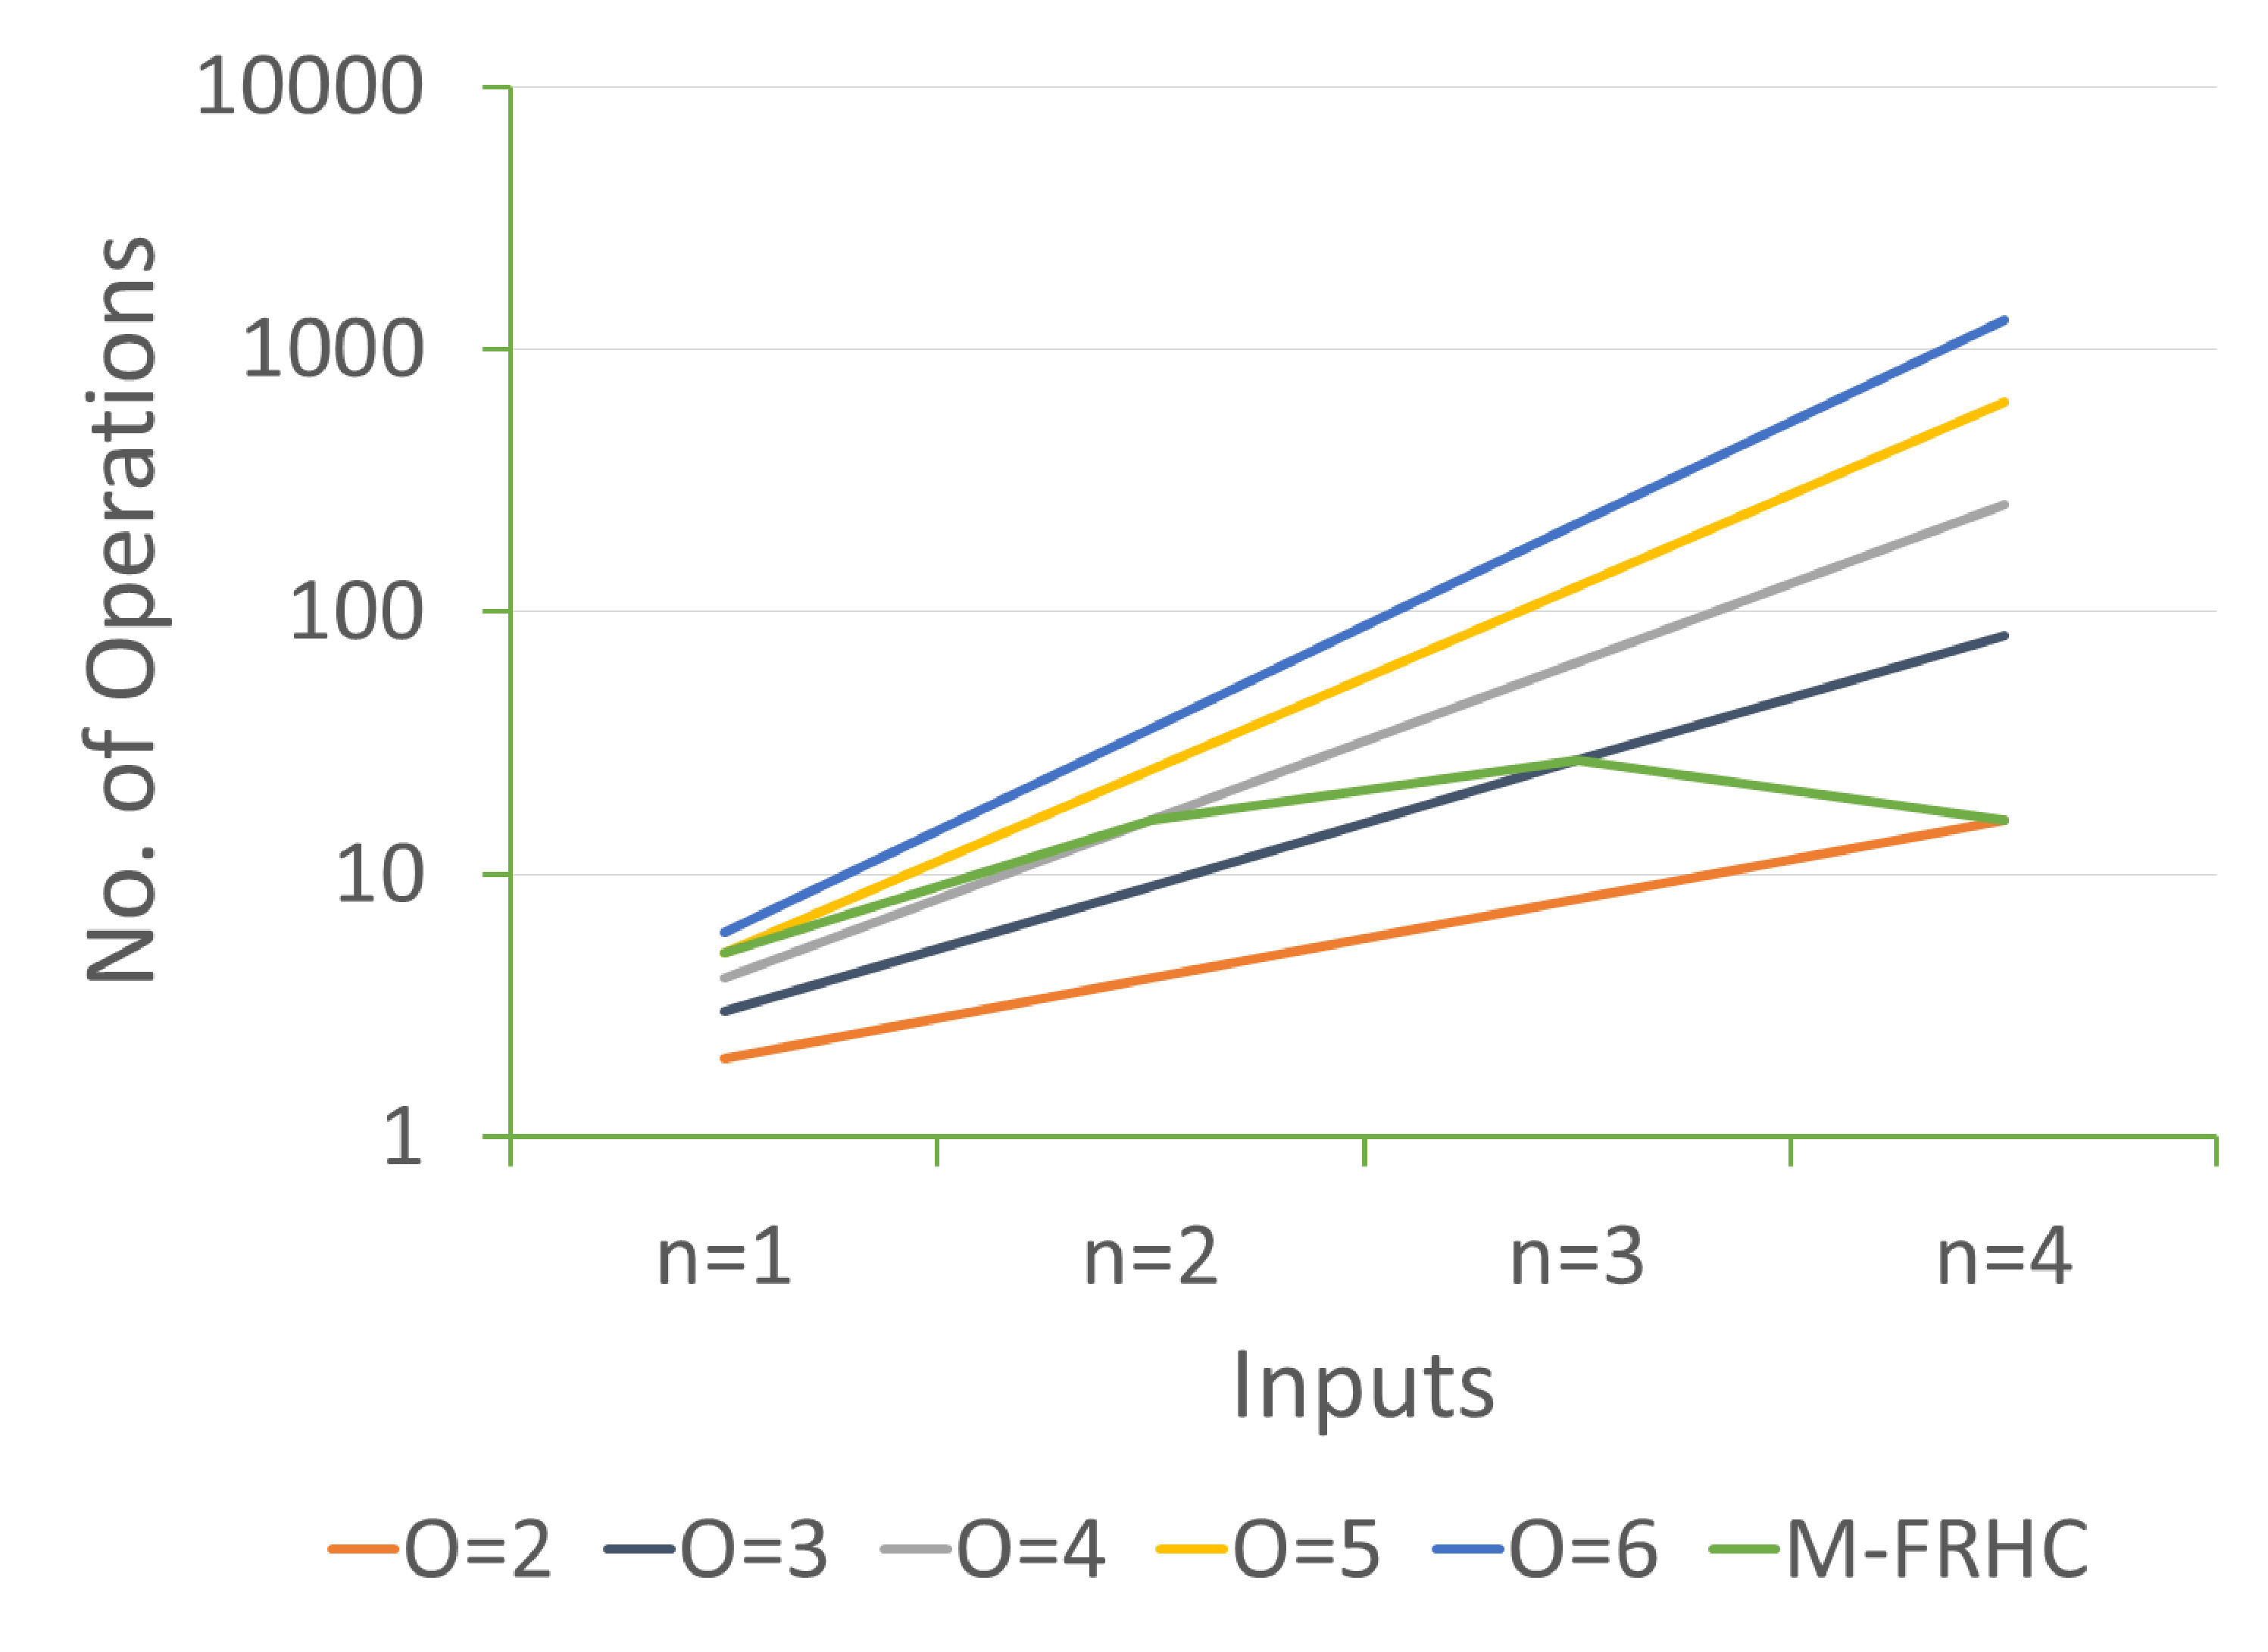
\includegraphics[width=0.95\linewidth]{Chapter2/chapter2/plot_MFRHC}
	\caption{Inputs vs No. of Operations with constant overlaps}
	\label{fig:plot_MFRHC}
\end{figure}

In G\hyp{}FLCS, implementation of M-FRHC will allow the number of overlaps to vary suitable with conjunction to the complexity of the control system. Here, $ n_{op} $ per fuzzy inference becomes a programmable parameter in this proposed M-FRHC rule reduction technique. The effect of this complexity reduction is presented in Figure \ref{fig:plot_MFRHC}. It can be observed that the number of fuzzy inferences or operations varies exponentially against the number of inputs considering a different number of overlapping membership functions except the plot corresponding to M-FRHC. In this G-FLCS implementation, $ \forall n = \left\{ {1,2,3,4} \right\} $, $ O={5,4,3,2} $. Using these values in \eqref{eq:ncells}, in the proposed M-FRHC based G-FLCS design, $ N_{cells} =\left\{ {5,16,27,16} \right\}  $ This causes a slight drop in the green line in Figure 2.2 specially when value of n transits from 3 to 4. It is observed from Figure \ref{fig:plot_MFRHC}, that the plot corresponding to M-FRHC is considerably parallel to x-axis on a logarithmic scale where all others are linearly increasing. This implies that, M-FRHC generates a constant number of operations per inference for all inputs $ N \to [1,4] $ whereas, the complexity of the G-FLCS increases exponentially with the increase in the number of inputs. It also caters a flexibility of adjusting the uncertainties on the boundary between the fuzzy sets. Hereby, \eqref{eq:FRHC_O} can translated to \eqref{eq:FRHC_OM2}.

\begin{table}[h!]
	\centering
	\caption{Computed $n_{op}$ with varying Inputs and Overlaps}
	\begin{tabular}{c|ccccc}
		\hline  
		%				InputOverlap & 2 & 3 & 4 & 5 \\
		\noalign{\vskip 1mm} \diagbox{$N$}{$O_l$} & 2 & 3 & 4 & 5 & 6\\
		\hline \noalign{\vskip 1mm} 
		1 & 2 & 3 & 4 & 5 & 6\\
		2 & 4 & 9 & 16 & 25 & 36\\
		3 & 8 & 27 & 64 & 125 & 216\\
		4 & 16 & 81 & 256 & 625 & 1296\\ \noalign{\vskip 1mm} 
		\hline
	\end{tabular}
	\label{tab:Nops}
\end{table}

\begin{equation} \label{eq:FRHC_OM2}
\begin{array}{l}
{\psi _I} = \left[ {\begin{array}{*{20}{c}}
	{{\mu _1}\left( {{i_1}} \right)}& \cdots &{{\mu _{{o_l}}}\left( {{i_1}} \right)}\\
	\vdots & \ddots & \vdots \\
	{{\mu _1}\left( {{i_N}} \right)}& \cdots &{{\mu _{{o_l}}}\left( {{i_N}} \right)}
	\end{array}} \right]\\~\\
{P_I} = \left[ {\begin{array}{*{20}{c}}
	{{p_1}\left( {{i_1}} \right)}& \cdots &{{p_{{o_l}}}\left( {{i_1}} \right)}\\
	\vdots & \cdots & \vdots \\
	{{p_1}\left( {{i_N}} \right)}& \cdots &{{p_{{o_l}}}\left( {{i_N}} \right)}
	\end{array}} \right]
\end{array}
\end{equation}
where, there are $ O_l $ number of elements in $ \psi _I $. $ O_l $ represents the number of overlaps considered.

It is required to track the index of membership function and link it to the Rulebase matrix appropriately. Hereby, in this scheme it is required to implement the vector combination operation on $ {P_I} $ along with $ {\psi _I} $ to generate $ C_{{R_k}} $ and $ C_{{R_v}} $ respectively. $ {C_{{R_k}}} $ and $ {C_{{R_v}}} $ can be represented as

\[\begin{array}{l}
{C_{{R_k}}} = {\Lambda _c}\left( {{P_1},{P_2}, \ldots {P_N}} \right)\\
{C_{{R_v}}} = {\Lambda _c}\left( {{\psi _1},{\psi _2}, \ldots {\psi _N}} \right)
\end{array}\]
where $ \Lambda _c $ denotes the vector combination as defined in Lemma \ref{lem:VecComb}.

$ C_{{R_k}} $ is required to derive the index of the Rulebase matrix $ R_b $.  The index $ k_x $ of Rulebase matrix $ R_b $ can be derived by
\begin{equation}
{k_x} = \left\{ {\sum\limits_{j = 0}^{N - 1} {{C_{{R_k}}}\left( {x,j} \right),\forall x|x \to \left[ {1,{N^{{O_l}}}} \right]} } \right\}
\end{equation}
\\
\begin{equation} \label{eq:Rb_kx}
\begin{array}{l}
{R_b}\left( {{k_x}} \right) = {c_j}\\
{c_j} \to \left[ {1,M} \right]\forall j = \left\{ {1,2, \ldots {N_R}} \right\}
\end{array}
\end{equation}
\par
Finally, fuzzy output is derived from the following relationship. 
\begin{equation} \label{eq:MFRHC-final}
{\theta _f}({c_j}) = \bigcap\limits_{{k_x} = 0}^{n_{op} - 1} {\left( {{\theta _f}\left( {{R_b}\left( {{k_x}} \right)} \right),\left( {\bigcup\limits_{l = 0}^{N - 1} {\overrightarrow {{C_{{R_v}}}\left( l \right)} } } \right)} \right)} 
\end{equation}
where, $ {\theta _f} $ is  fuzzy output vector, index $ k_x $ varying from $ 0  $ to number of fuzzy operations $ (n_{op} - 1) $, $ R_b $ is the rule base matrix, $ C_{R_V} $ represents the vector combination of non-zero fuzzified input values, $ l $ varying from $ 0 $ to $ N-1 $ and $ \bigcap {} $  and $ \bigcup {} $ representing t-norm and s-norm operations respectively. It is important to analyze the data path of the system architecture to take advantage of the device architecture on which it will be deployed. The target processor is a VLIW based DSP device. The system architecture can be modified at later stage however, there should be scope for data and instruction level parallelism. 

\subsection{Modified and Thresholded Fired Rulebase Hyper Cube (MT-FRHC)}
In this section, MT-FRHC is proposed to tackle the challenges of removing unwanted firing of rules by insignificantly close to zero fuzzy values. The removal of these rules significantly increases computational speed without affecting the output accuracy. This can be achieved by introducing a threshold in \eqref{eq:FRHC_OM2}. Consider an element in $ {\psi _I} $ that assume a very low value and eventually may fire one or more rules. Based on T-Norm operators, weights of all these fired rules are likely to be close to the value of the element. This value will produce a minuscule $ \lambda $ cut-set at the fuzzy output set if there exist no value greater than the current weight assigned to the corresponding member of the fuzzy set. The effect of this $ \lambda $ cut-set is likely to result in a very fine change in output after defuzzification. Thus analytically, it is beneficial to remove these values from  $ {\psi _I} $ based on a suitable threshold.  

Considering all elements of ${\psi _I} $ is greater than threshold $ \tau $, ${\psi _I}^T $ can be computed as 
\begin{align} \label{eq:MTFRHC}
{\psi _I}^T = \{ {d_{jq}}|&({d_{jq}} \in {\psi _I},\forall j \to [1,{O_l}],q \to [1,N]) \\ \nonumber
&\text{ and }{d_{jq}} > \tau \}
\end{align} 
This implies,
\[{d_{jq}} \notin {\psi _I}\forall {d_{jq}} < \tau \]
where, $ {d_{jq}} $ represents individual elements of matrix $ {\psi _I}^T $.
As the elements in $ {\psi _I} $ decreases, the row vectors in $ {C_{{R_v}}} $ and $ {C_{{R_k}}} $ decreases. The number row vectors is equal to $ n_{op}  $ and thus it can be inferred that $ \tau $ is inversely proportional to the computational complexity.

Consider the following example where the rules are 
\[\begin{array}{l}
If~input~I~is~M{F_1}~then~Output~O~is~{P_1}\\
If~input~I~is~M{F_2}~then~Output~O~is~{P_2}\\
If~input~I~is~M{F_3}~then~Output~O~is~{P_3}
\end{array}\]
and the input space is fuzzy partitioned as in Figure \ref{fig:MTFRHC_plot_2}.
\begin{figure}[h]
\centering
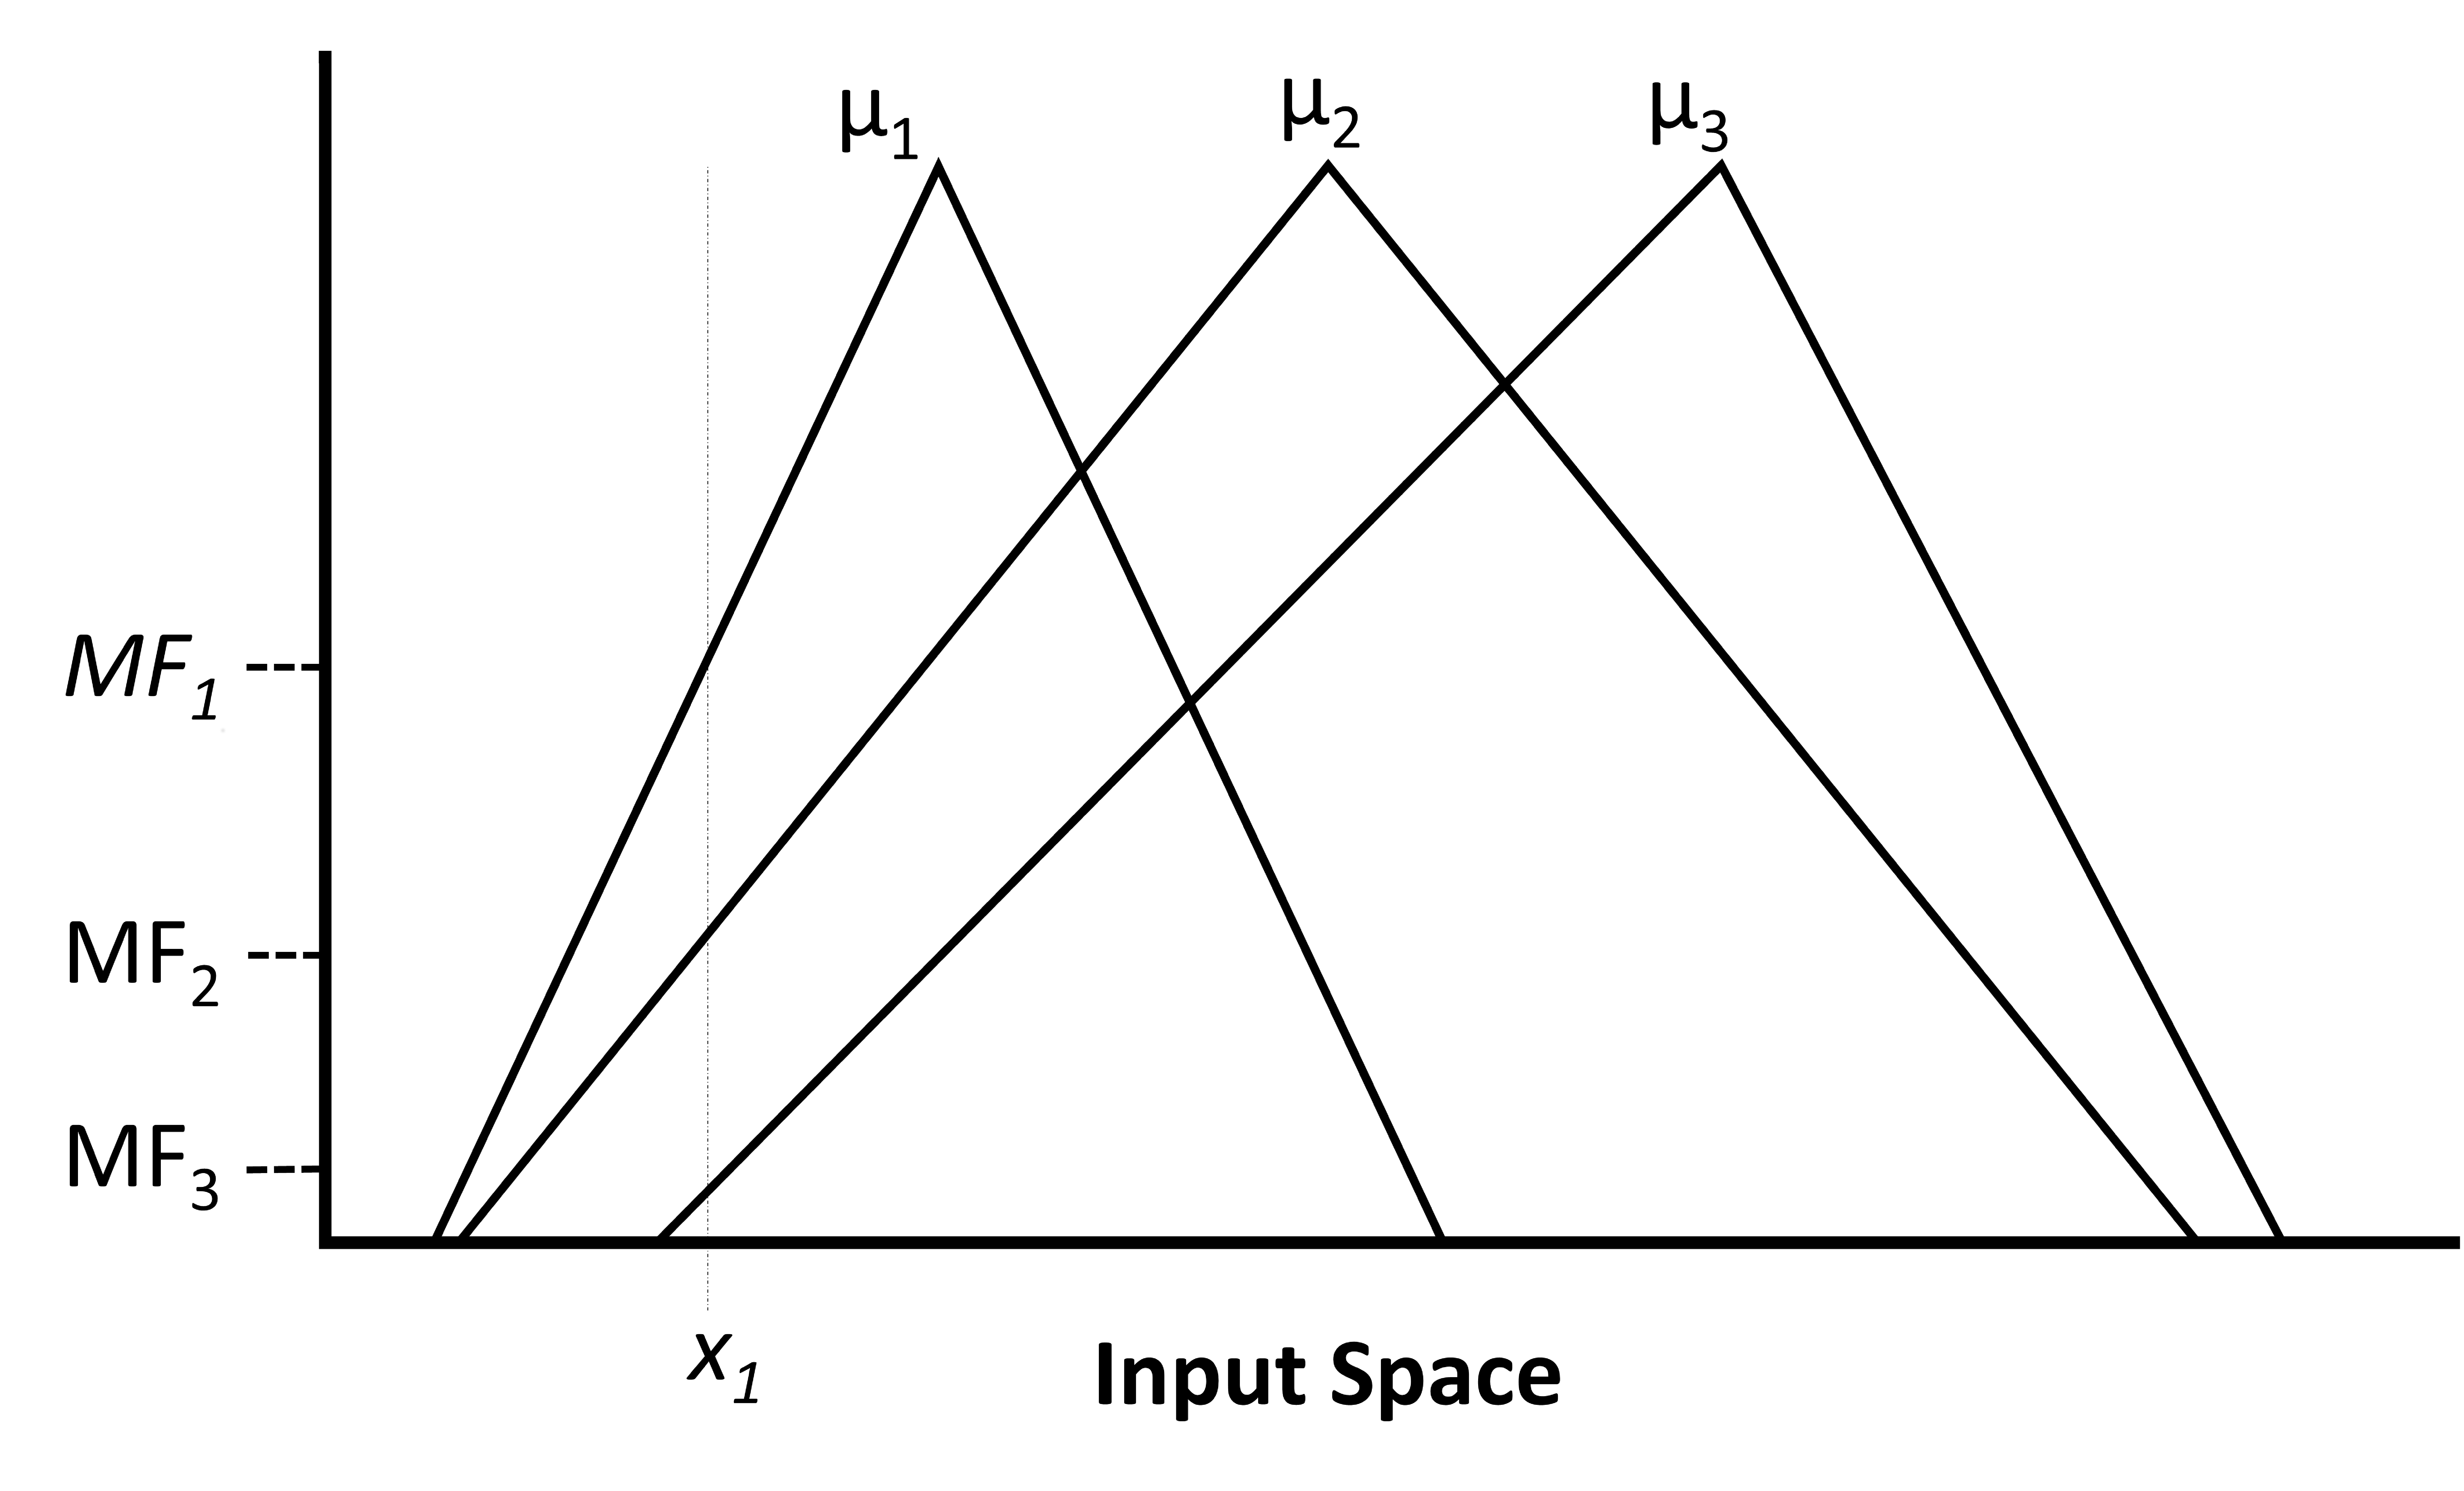
\includegraphics[width=0.7\linewidth]{Chapter2/chapter2/MTFRHC_plot_2}
\caption{An Example: Input Membership Function}
\label{fig:MTFRHC_plot_2}
\end{figure}

Assuming, $N_Cells=5$ with one input and the input value being $x_1$, the M-FRHC output is,
\[\left [M{F_1},~M{F_2},~M{F_3}\right ]\]
It is obvious from  Figure \ref{fig:MTFRHC_plot_2} that, $ M{F_1}>M{F_2}>M{F_3} $. Now if $M{F_3}$ is very very small, then its effect on the output is small. However, due to its firing, an additional rule is active and it gets evaluated. This evaluated rule is extremely weak as the weight it carries (from $M{F_3}$) is very small. Thus, if this rule is excluded from the computation, the accuracy of the system does not change much, but the reduction in computation is reduced by one-third(instead of 3 rules, only 2 rules are evaluated) in above example. Thus in MT-FRHC, a threshold $\tau $ is expended to discard rules which carry extremely small weight.


\section{Defuzzification}
\begin{figure}[b!]
\centering
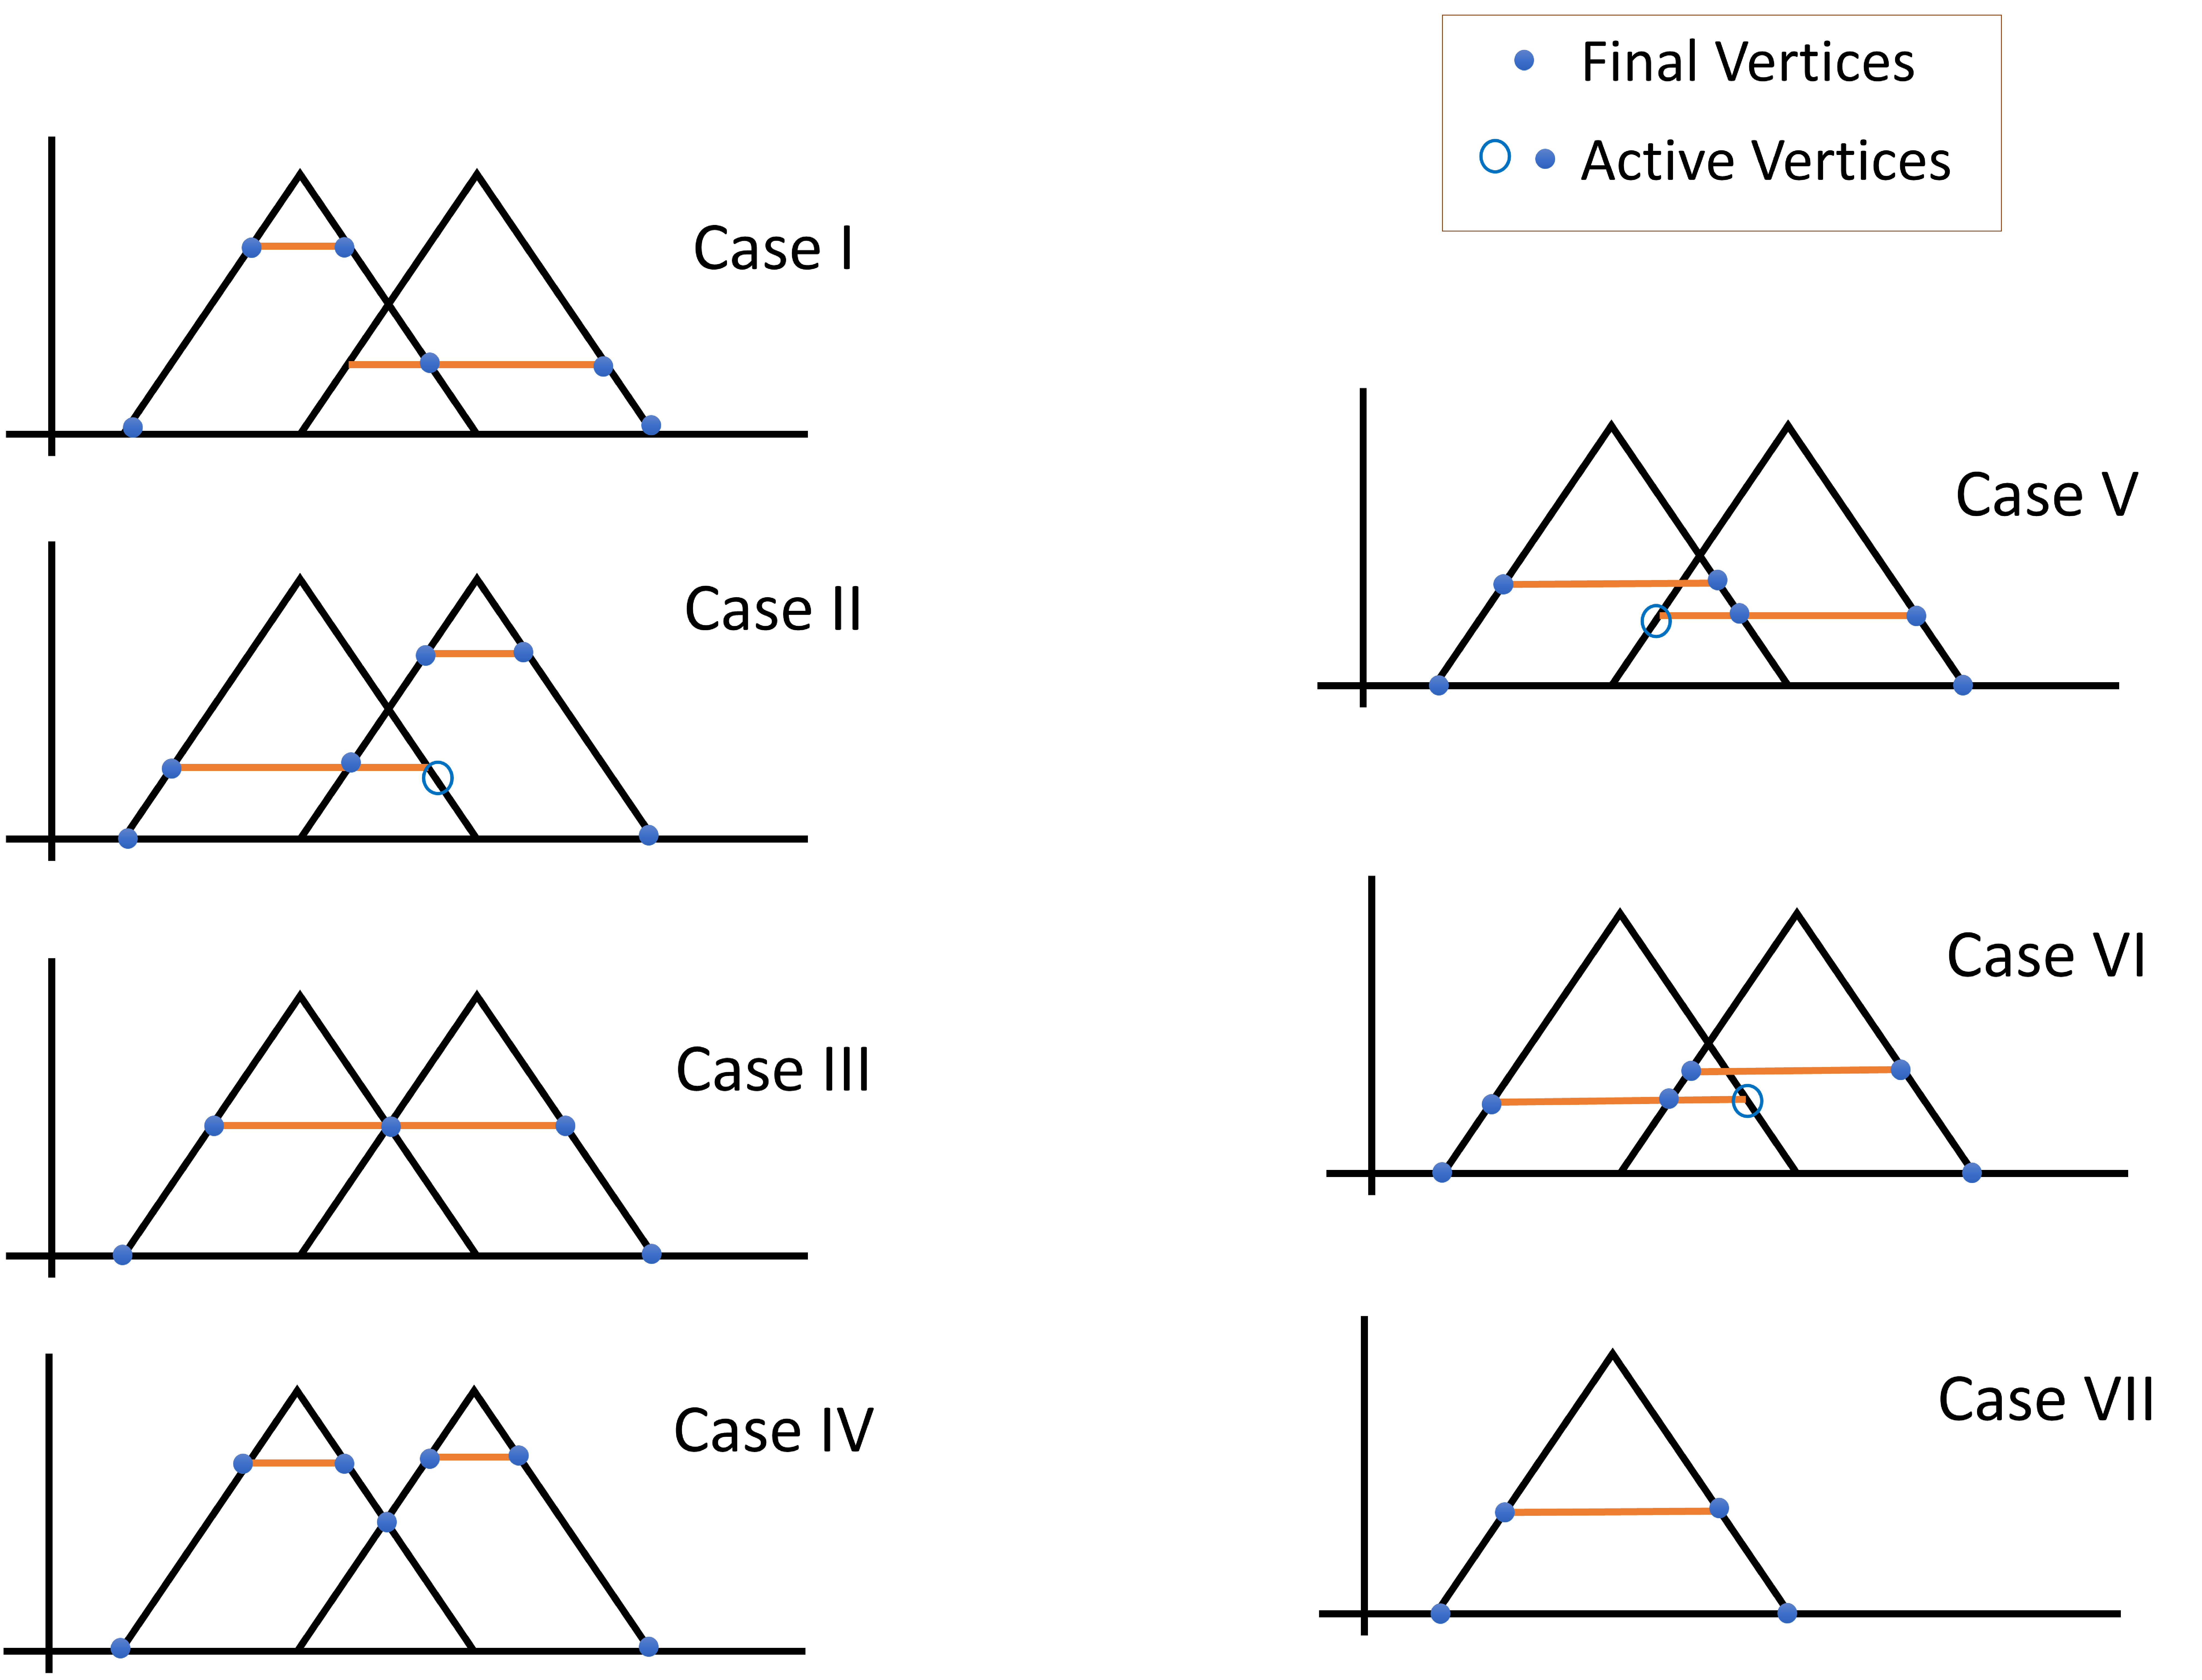
\includegraphics[width=1\textwidth,,height=15cm]{Chapter2/chapter2/Vertices_cases}
\caption{Various cases for vertices computation for Centroid of Area (COA) Defuzzification}
\label{fig:Vertices_cases}
\end{figure}

As discussed in the earlier section, to generate a quantifiable output using fuzzy logic that can be implied in a real system, defuzzification process is obligatory. Inference engine in a FLCS will have a number of rules that transform variables into a fuzzy result described in terms of membership in fuzzy sets. The defuzzification process converts output expressed in fuzzy sets to crisp output using MFs. It employs certain mathematical operations to interpret the membership degrees of the fuzzy sets into a particular decision or real value. There are number of defuzzification algorithms in literature \cite{Saletic2006,Ross2010,Lee1990,Lee1990a}. The varied processes of defuzzification yields different crisp output. The most widely used defuzzification methods are discussed further.

\subsection{Defuzzification Algorithms}
Leekwijck et. al. \cite{Leekwijck1999} classified defuzzification methods broadly in to 
\begin{enumerate}
	\item Maxima methods and its derivatives,
	\item Distribution methods and its derivatives,
	\item Area methods, and
	\item Miscellaneous methods.
\end{enumerate}
Leekwijck et. al. claim that the \textit{Maxima} methods are suitable candidates for fuzzy reasoning systems whereas the \textit{Area} methods display the attribute of continuity that makes them appropriate for FLCs. Zavala et. al.\cite{Zavala2011} states that among numerous different defuzzification methods available in literature, most used for hardware purposes are Center of Area (CoA) which is classified under Area methods and Mean Of Maxima which is classified under Maxima methods. WA defuzzification method is the also among most frequently used defuzzification technique which is classified under Area methods. Therefore, since our target applications are fuzzy control, CoA and weighted average (WA) is ultimately chosen as the defuzzification method for proposed hardware G\hyp{}FLCS. 

\subsubsection{Weighted Average Defuzzification Technique}
WA defuzzification method is the most frequently used defuzzification technique for fuzzy controllers owing to its low computational complexity. It can even be easily implemented on slow processors like microcontrollers for real-time applications. But this technique can be applied to symmetrical output MFs. The WA method is computed by weighting each output MF by its respected maximum MF value and accumulating them. This can be represented as,
\[{X_{WA}} = \frac{{\sum {{\mu _{\widetilde C}}\left( {\overline x } \right) \cdot \overline x } }}{{\sum {{\mu _{\widetilde C}}\left( {\overline x } \right)} }}\]
where $ \overline x $ represents centroid of each symmetric output MF $ {\widetilde C} $. It is generally not used for G-FLCS with asymmetric output MFs \cite{Ross2010}. Although there are many instances where this method is used for FLCs with asymmetric output MFs \cite{Sugeno1985}.

\subsubsection{CoA Defuzzification Technique}
CoA method is commonly known as center of gravity (CoG) defuzzification. It was developed by Sugeno in 1985\cite{Sugeno1985}. CoA is most commonly used technique in fuzzy control and provides good accuracy \cite{Ross2010,Patel2002}. 
Mathematically this technique is represented as
\[{X_{CoA}} = \frac{{\int {{\mu _c}(x)xdx} }}{{\int {{\mu _c}(x)dz} }}\]
where $ {\mu _c}(x)  $ represents membership degree of each output MF.
Continuity and computational efficiency are of utmost importance for hardware G\hyp{}FLCS. In most realization of CoA, calculating the whole area and determining where its weighted midpoint is essential. As it uses all elements from input universe, it requires $ k = {2^n} - 1 $ iterations according to number of bits ($ n $) used for input universe. These techniques aim at reducing resource consumption and computational time without loss of accuracy. 
Some hardware implementation for CoA uses Center of Slice Area Average (COSAA)defuzzification technique proposed by Zavala et. al. \cite{Zavala2011,HernandezZavala2013,Zavala2010}. COSAA uses the summation of midpoints for all $ \alpha - $ levels instead of integrating the area under a curve. 

\subsection{Vertices based Center of Area (VBCoA) Computation}
The existing techniques for defuzzification using CoA have been seen to be computationally time-consuming. One of the most widely used technique is the Riemann sum based CoA computation. Riemann integral is used for deriving the centroid of area in actual method \cite{Patel2002,Leekwijck1999}. Centroid of a polygon can also be computed using their vertices and has been widely used in geospatial applications \cite{Stankute2010}. This feature is used in the proposed VBCoA defuzzification method. To reduce the defuzzification time, a new vertices based CoA (VBCoA) computation method is proposed. The proposed method can be implemented in following steps.
\begin{description}
	\item[Step 1] Generate cut set matrix from all cut points with non-zero fuzzy output values.
	\item[Step 2] Use cut set to segregate into any one of cases as presented in Figure \ref{fig:Vertices_cases}.
	\item[Step 3] Generate intersecting matrix. Intersecting matrix includes intersecting points of output MF.
	\item[Step 4] Generate individual set of vertices from intersecting matrix and cut set matrix for various case structures as in Figure \ref{fig:Vertices_cases}.
	\item[Step 5] Centroid on X-axis can be calculated as 
	\[\begin{array}{l}
	COA = \frac{1}{{6A}}\sum\limits_{i = 0}^{n - 1} {\left( {{y_i} + {y_{i + 1}}} \right)} \left( {{x_i}{y_{i + 1}} - {x_{i + 1}}{y_i}} \right)\\
	A = \frac{1}{2}\sum\limits_{i = 0}^{n - 1} {\left( {{x_i}{y_{i + 1}} - {x_{i + 1}}{y_i}} \right)} 
	\end{array}\]
	where $n\rightarrow $number of vertices, $ x_i\rightarrow $ $ x $ co-ordinate of $ i^{th} $ vertex, $ y_i\rightarrow $ $ y $ co-ordinate of $ i^{th} $ vertex
\end{description}

The steps 1 through 5 can be used to defuzzify fuzzy output $\theta _f$ using COA process in a fast and efficient manner\footnote{Download Code Here: https://goo.gl/83bVna}. The proposed VBCoA defuzzification algorithm and the traditional Riemann sum based defuzzification algorithm were implemented on a C6748 DSP processor with 300 MHz operating frequency. To analyze the efficacy of the proposed algorithm, computation time using the VBCoA were compared to existing Riemann sum based CoA computation technique. A random set of fuzzy output was generated and defuzzified using these two methods. The process was repeated for five times and he observed cycle time is tabulated in Table \ref{tab:centComp}. The randomly generated fuzzy output set appears in the first row of the table. The next two rows shows the consumed cycles and the cycle time (in $\mu$s) respectively for traditional Riemann sum based CoA computation. The final two rows shows the consumed cycles and the cycle time (in $\mu$s) respectively for the proposed VBCoA computation. Table \ref{tab:centComp} reflects that the proposed VBCoA technique provides a slightly better performance in terms of computational time. VBCoA shows approximately 30\% improvement in the cycle time.

 \begin{table}[h]
 	\centering
 	\caption{Centroid computation on C6748 DSP Hardware}
 	\label{tab:centComp}
% 	\resizebox{1\textwidth}{!}{%
 		\begin{tabular}{c|cc|cc}
 			\hline \noalign{\vskip 1mm}
 			\multirow{2}{*}{} & \multicolumn{2}{c|}{Riemann sum} & \multicolumn{2}{c|}{\textbf{VBCoA} Method} \\ \cline{2-5} \noalign{\vskip 1mm}
 			& Cycles & Time($\mu$s) & Cycles & Time($\mu$s) \\ \hline \noalign{\vskip 1mm}
 			{[}0.2,0.5,0.3{]} & 7662 & 25.54 & 5316 & 17.72 \\  \noalign{\vskip 1mm} 
 			{[}0.4,0.3,0.1{]} & 7681 & 25.60 & 5320 & 17.73 \\  \noalign{\vskip 1mm} 
 			{[}0.8,0.8,0.6{]} & 7528 & 25.54 & 5305 & 17.68 \\  \noalign{\vskip 1mm} 
 			{[}0.1,0.7,0.1{]} & 7650 & 25.50 & 5316 & 17.72 \\  \noalign{\vskip 1mm} 
 			{[}0.3,0.2,0.9{]} & 7677 & 25.59 & 5309 & 17.70 \\  \noalign{\vskip 1mm} \hline
 		\end{tabular}
% 	}
 \end{table}
		

\section{Performance Analysis}

%scale=0.1
\begin{figure}[htbp]
	\centering
	\subfloat[Fuzzy PI Approximation FIS: MT-FRHC]{\label{fig:SPlot_MT-FRHC}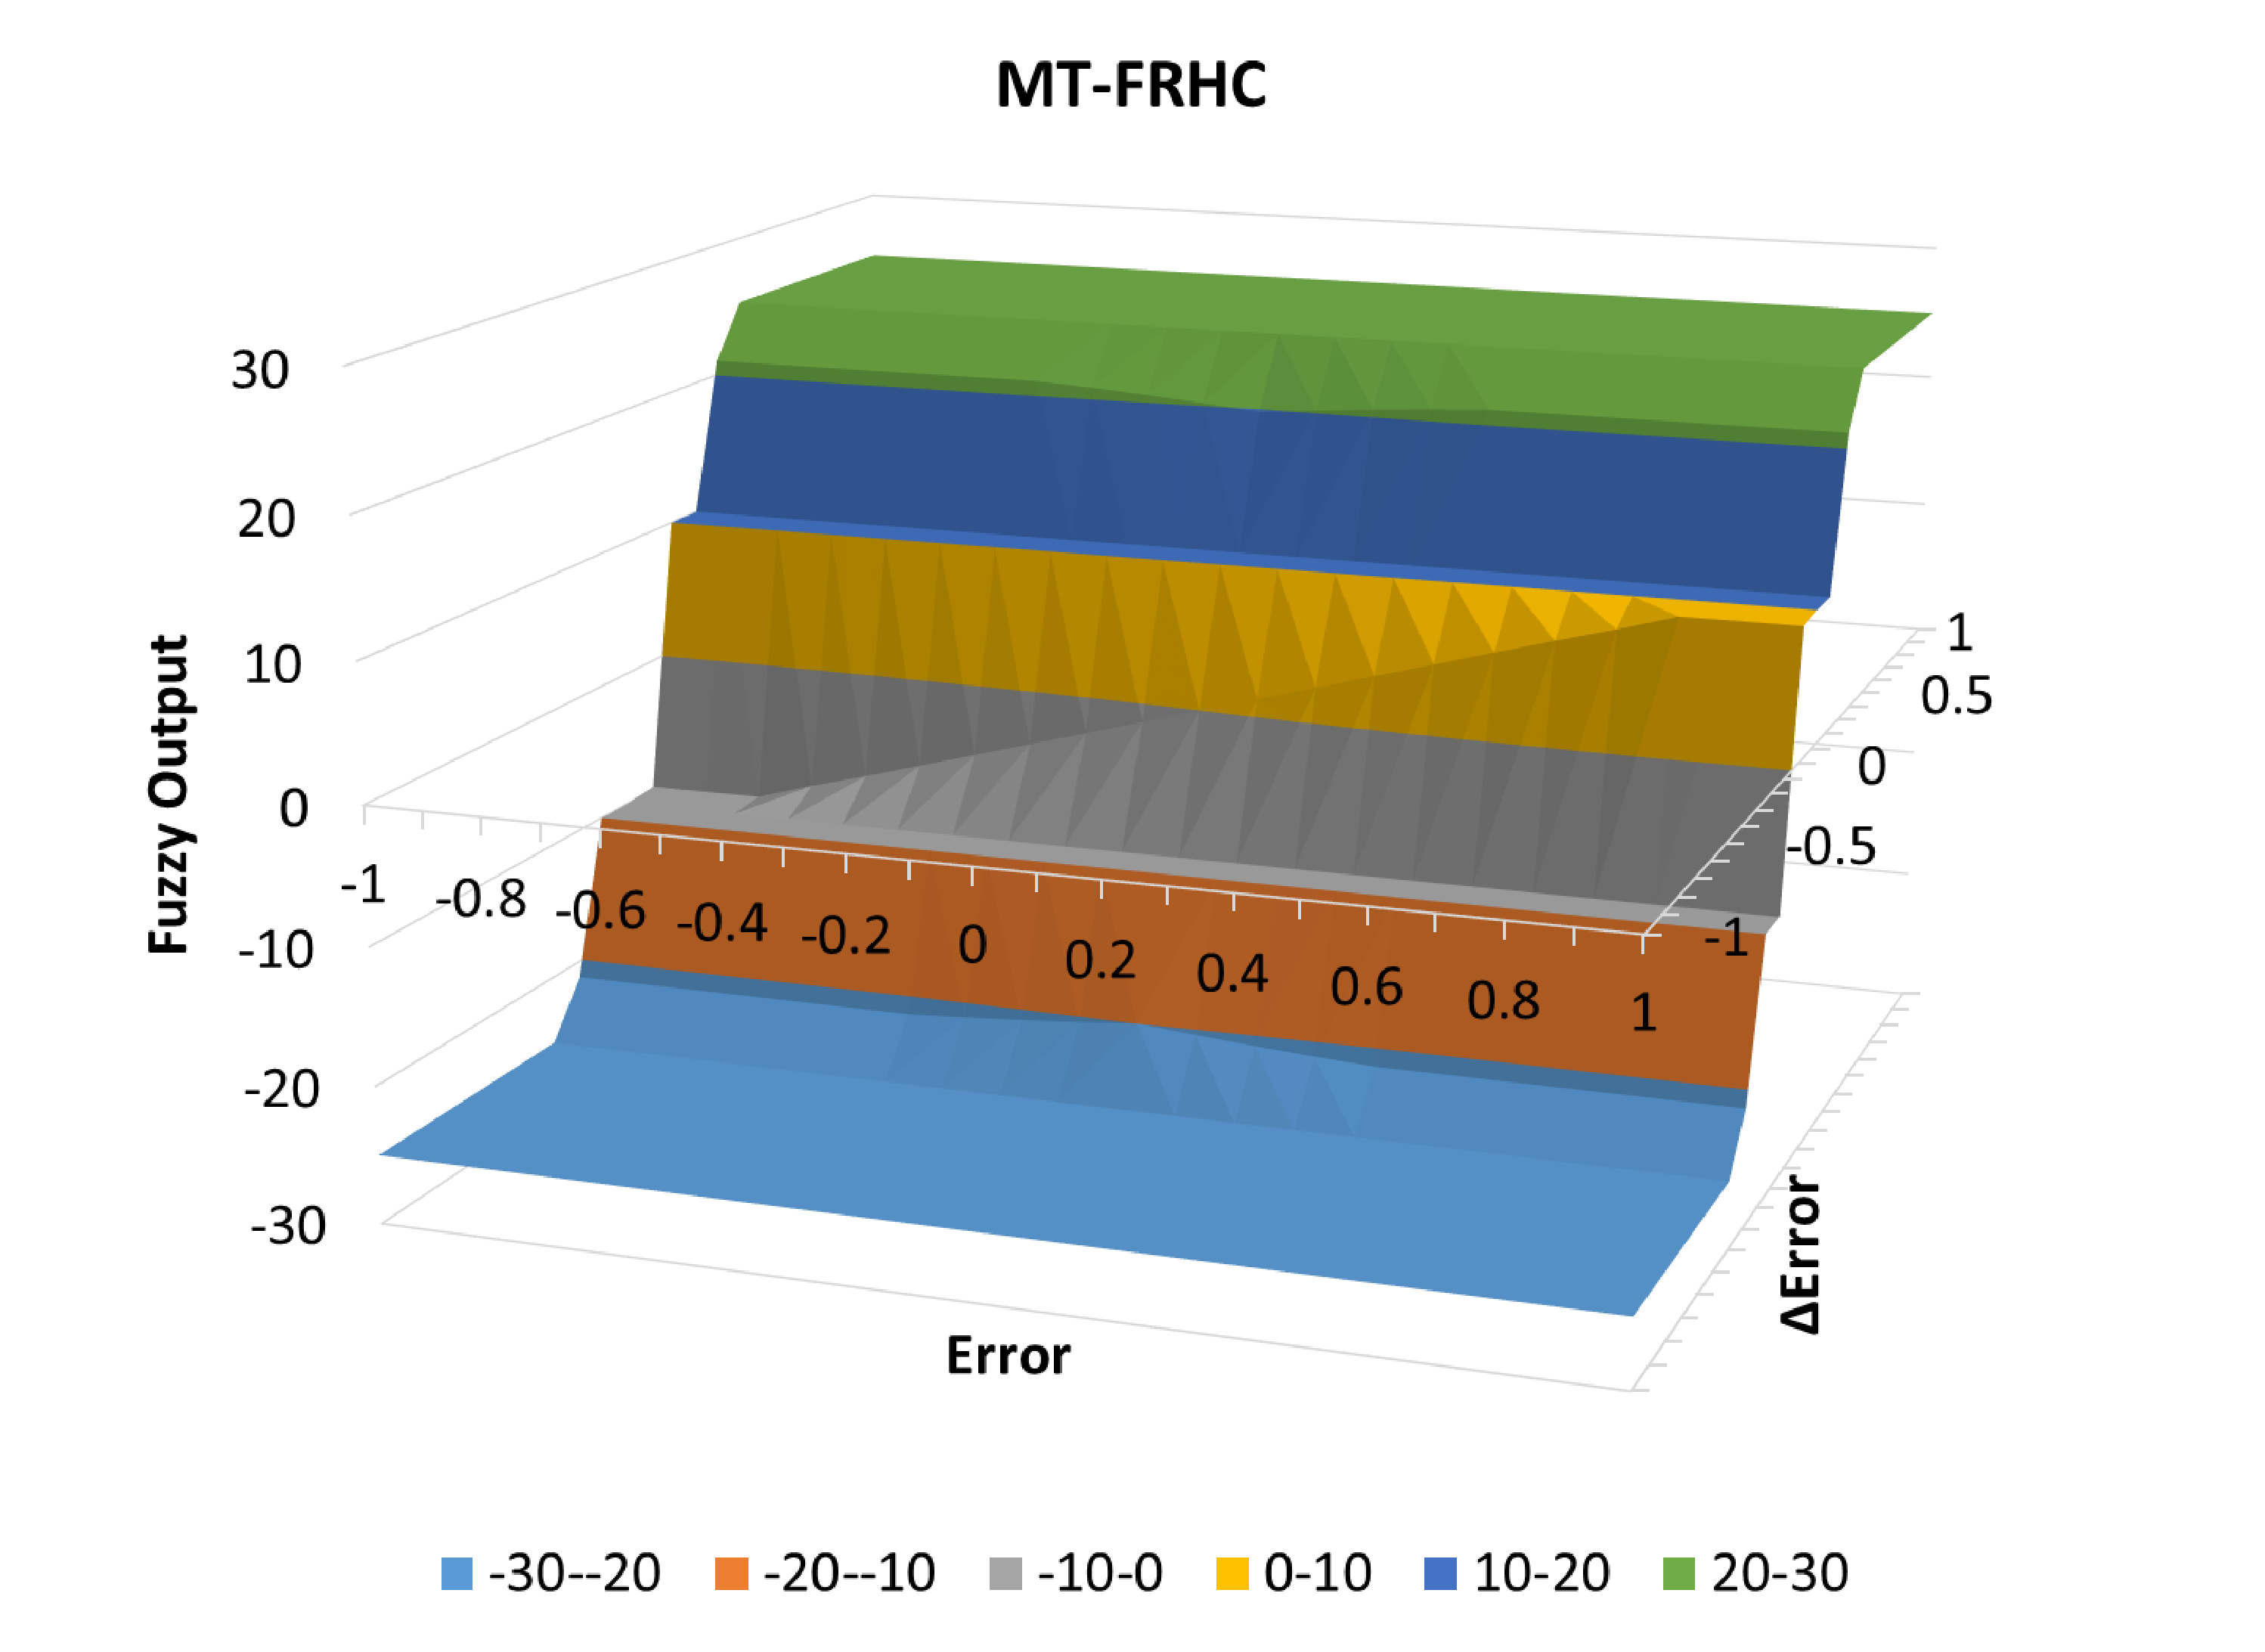
\includegraphics[width=0.6\linewidth]{Chapter2/chapter2/MTFRHC_plot.eps}} \\
	\subfloat[Fuzzy PI Approximation FIS: Matlab Fuzzy Toolbox]{\label{fig:SPlot_MFT}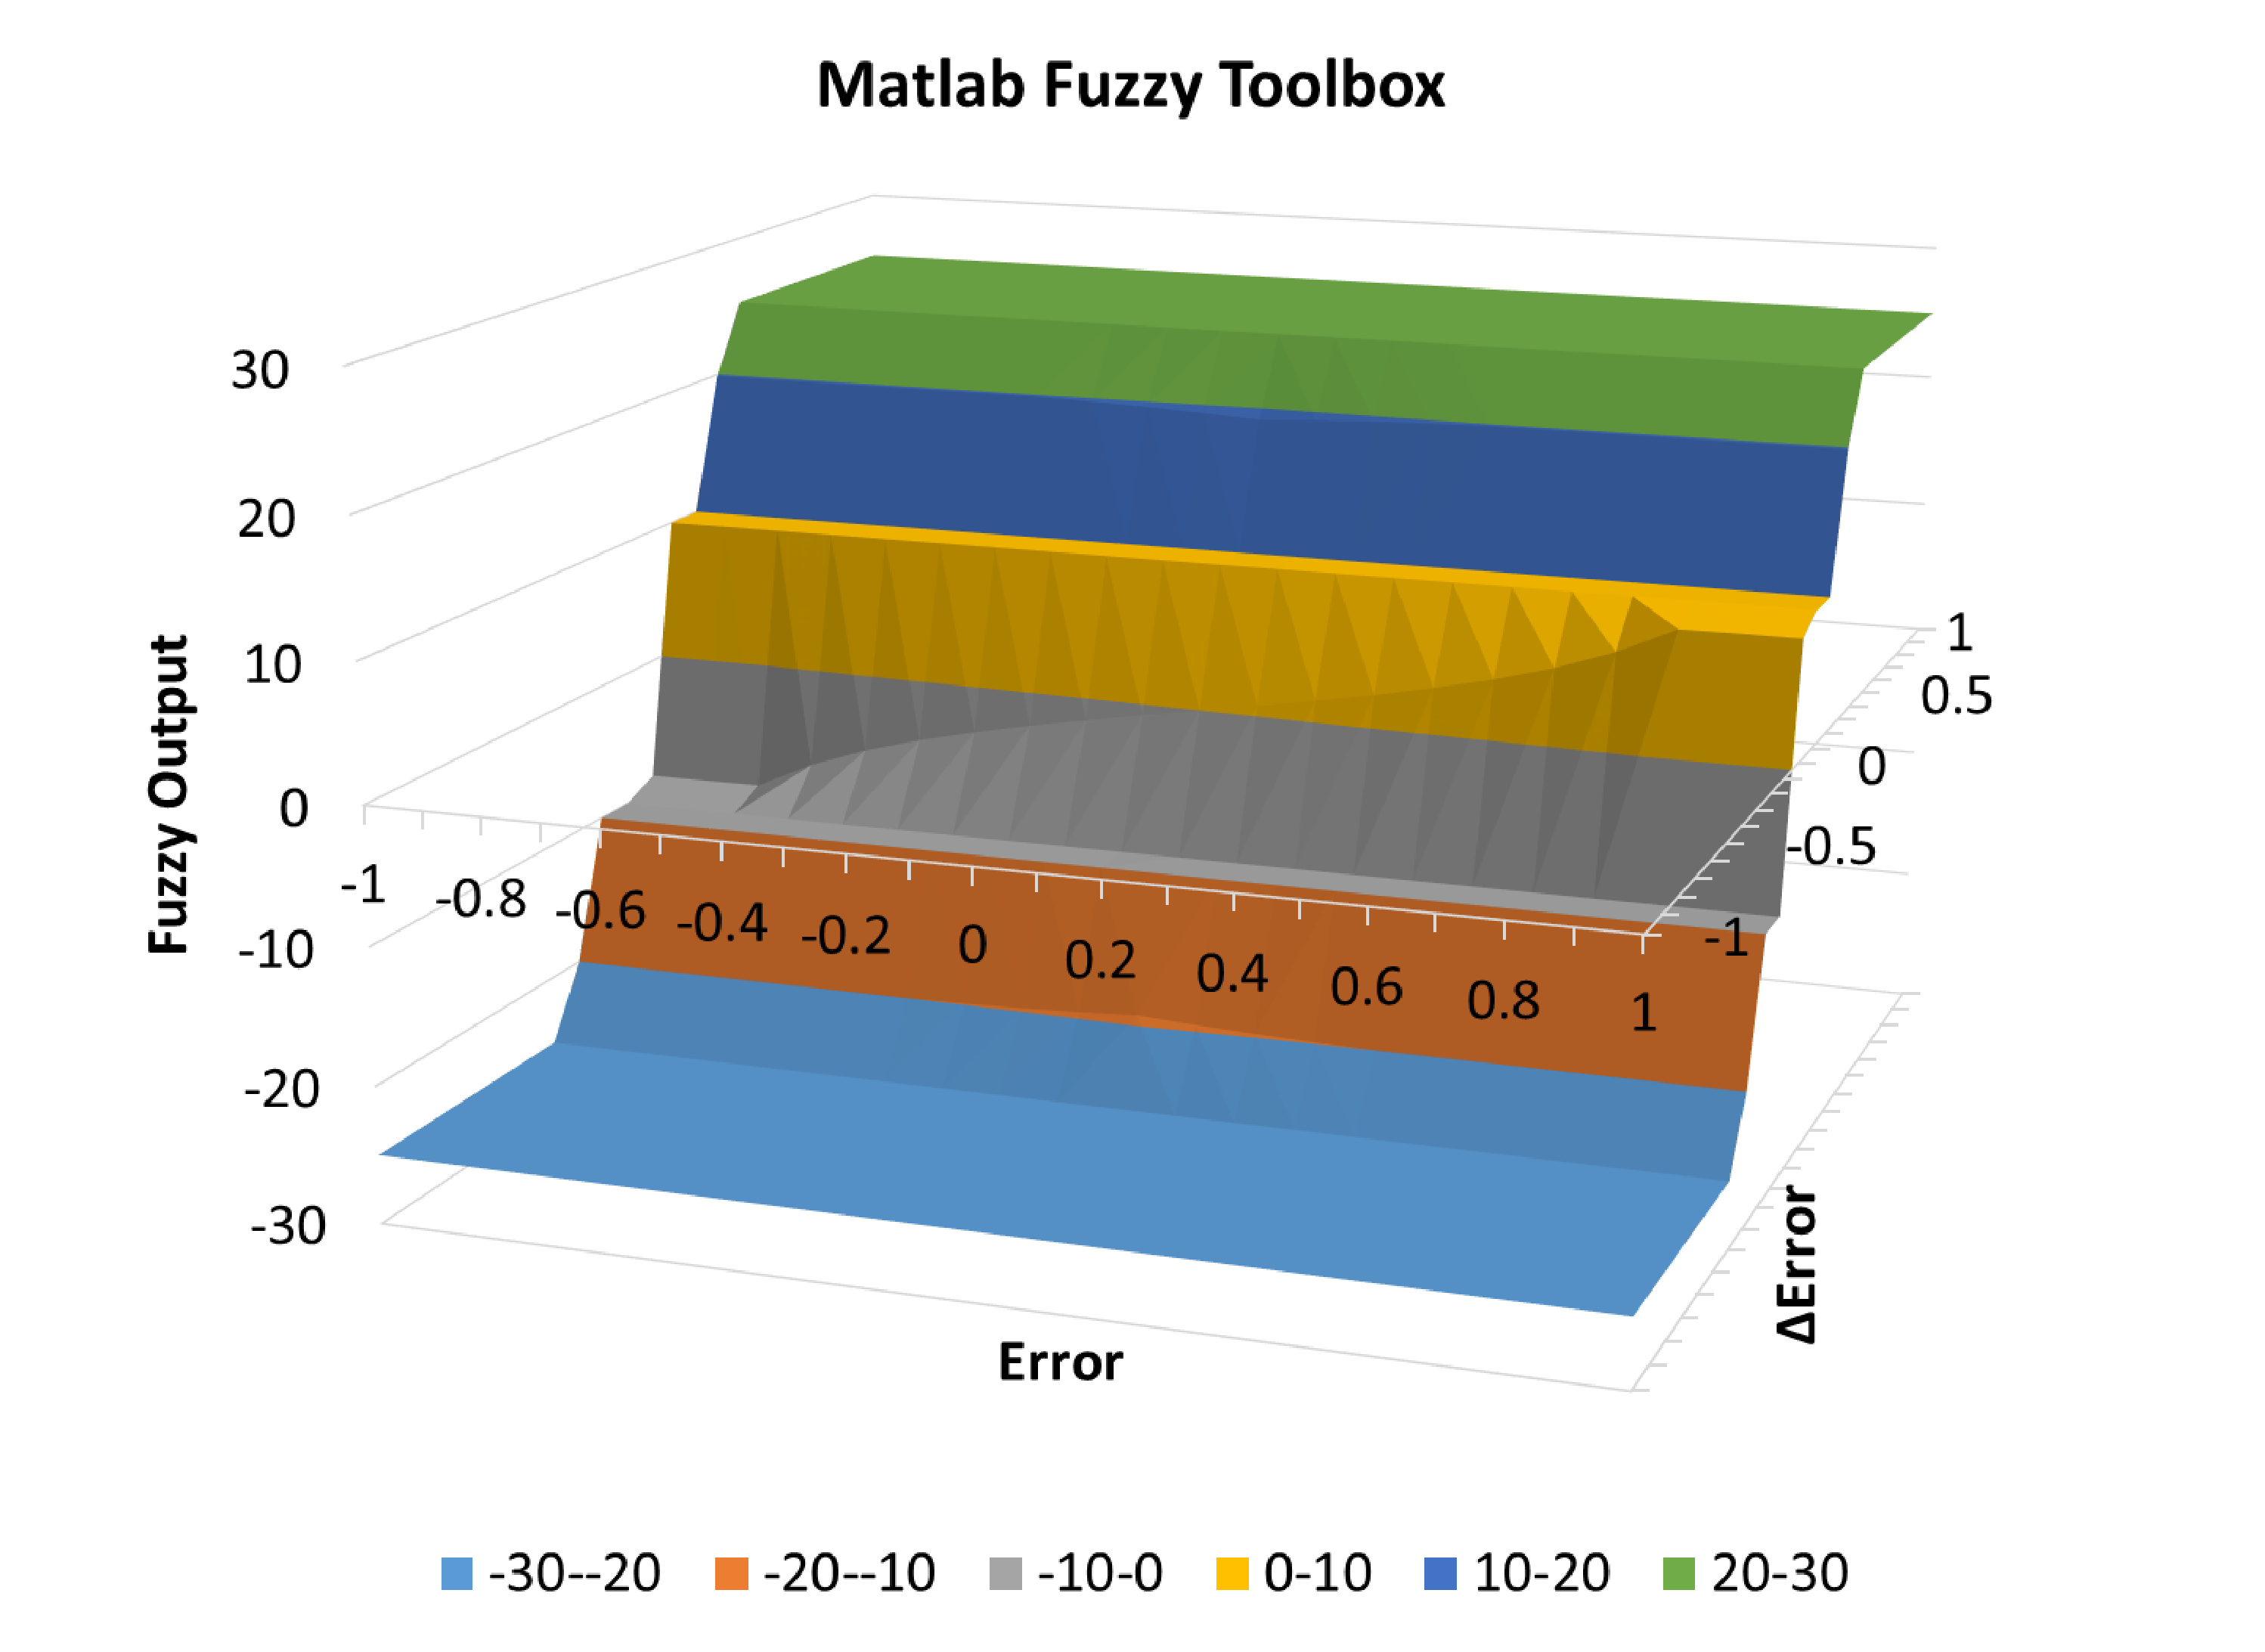
\includegraphics[width=0.6\linewidth]{Chapter2/chapter2/MatlabToolbox_plot.eps}} \\
	\subfloat[Fuzzy PI Approximation FIS: Error Plot]{\label{fig:SPlot_Error}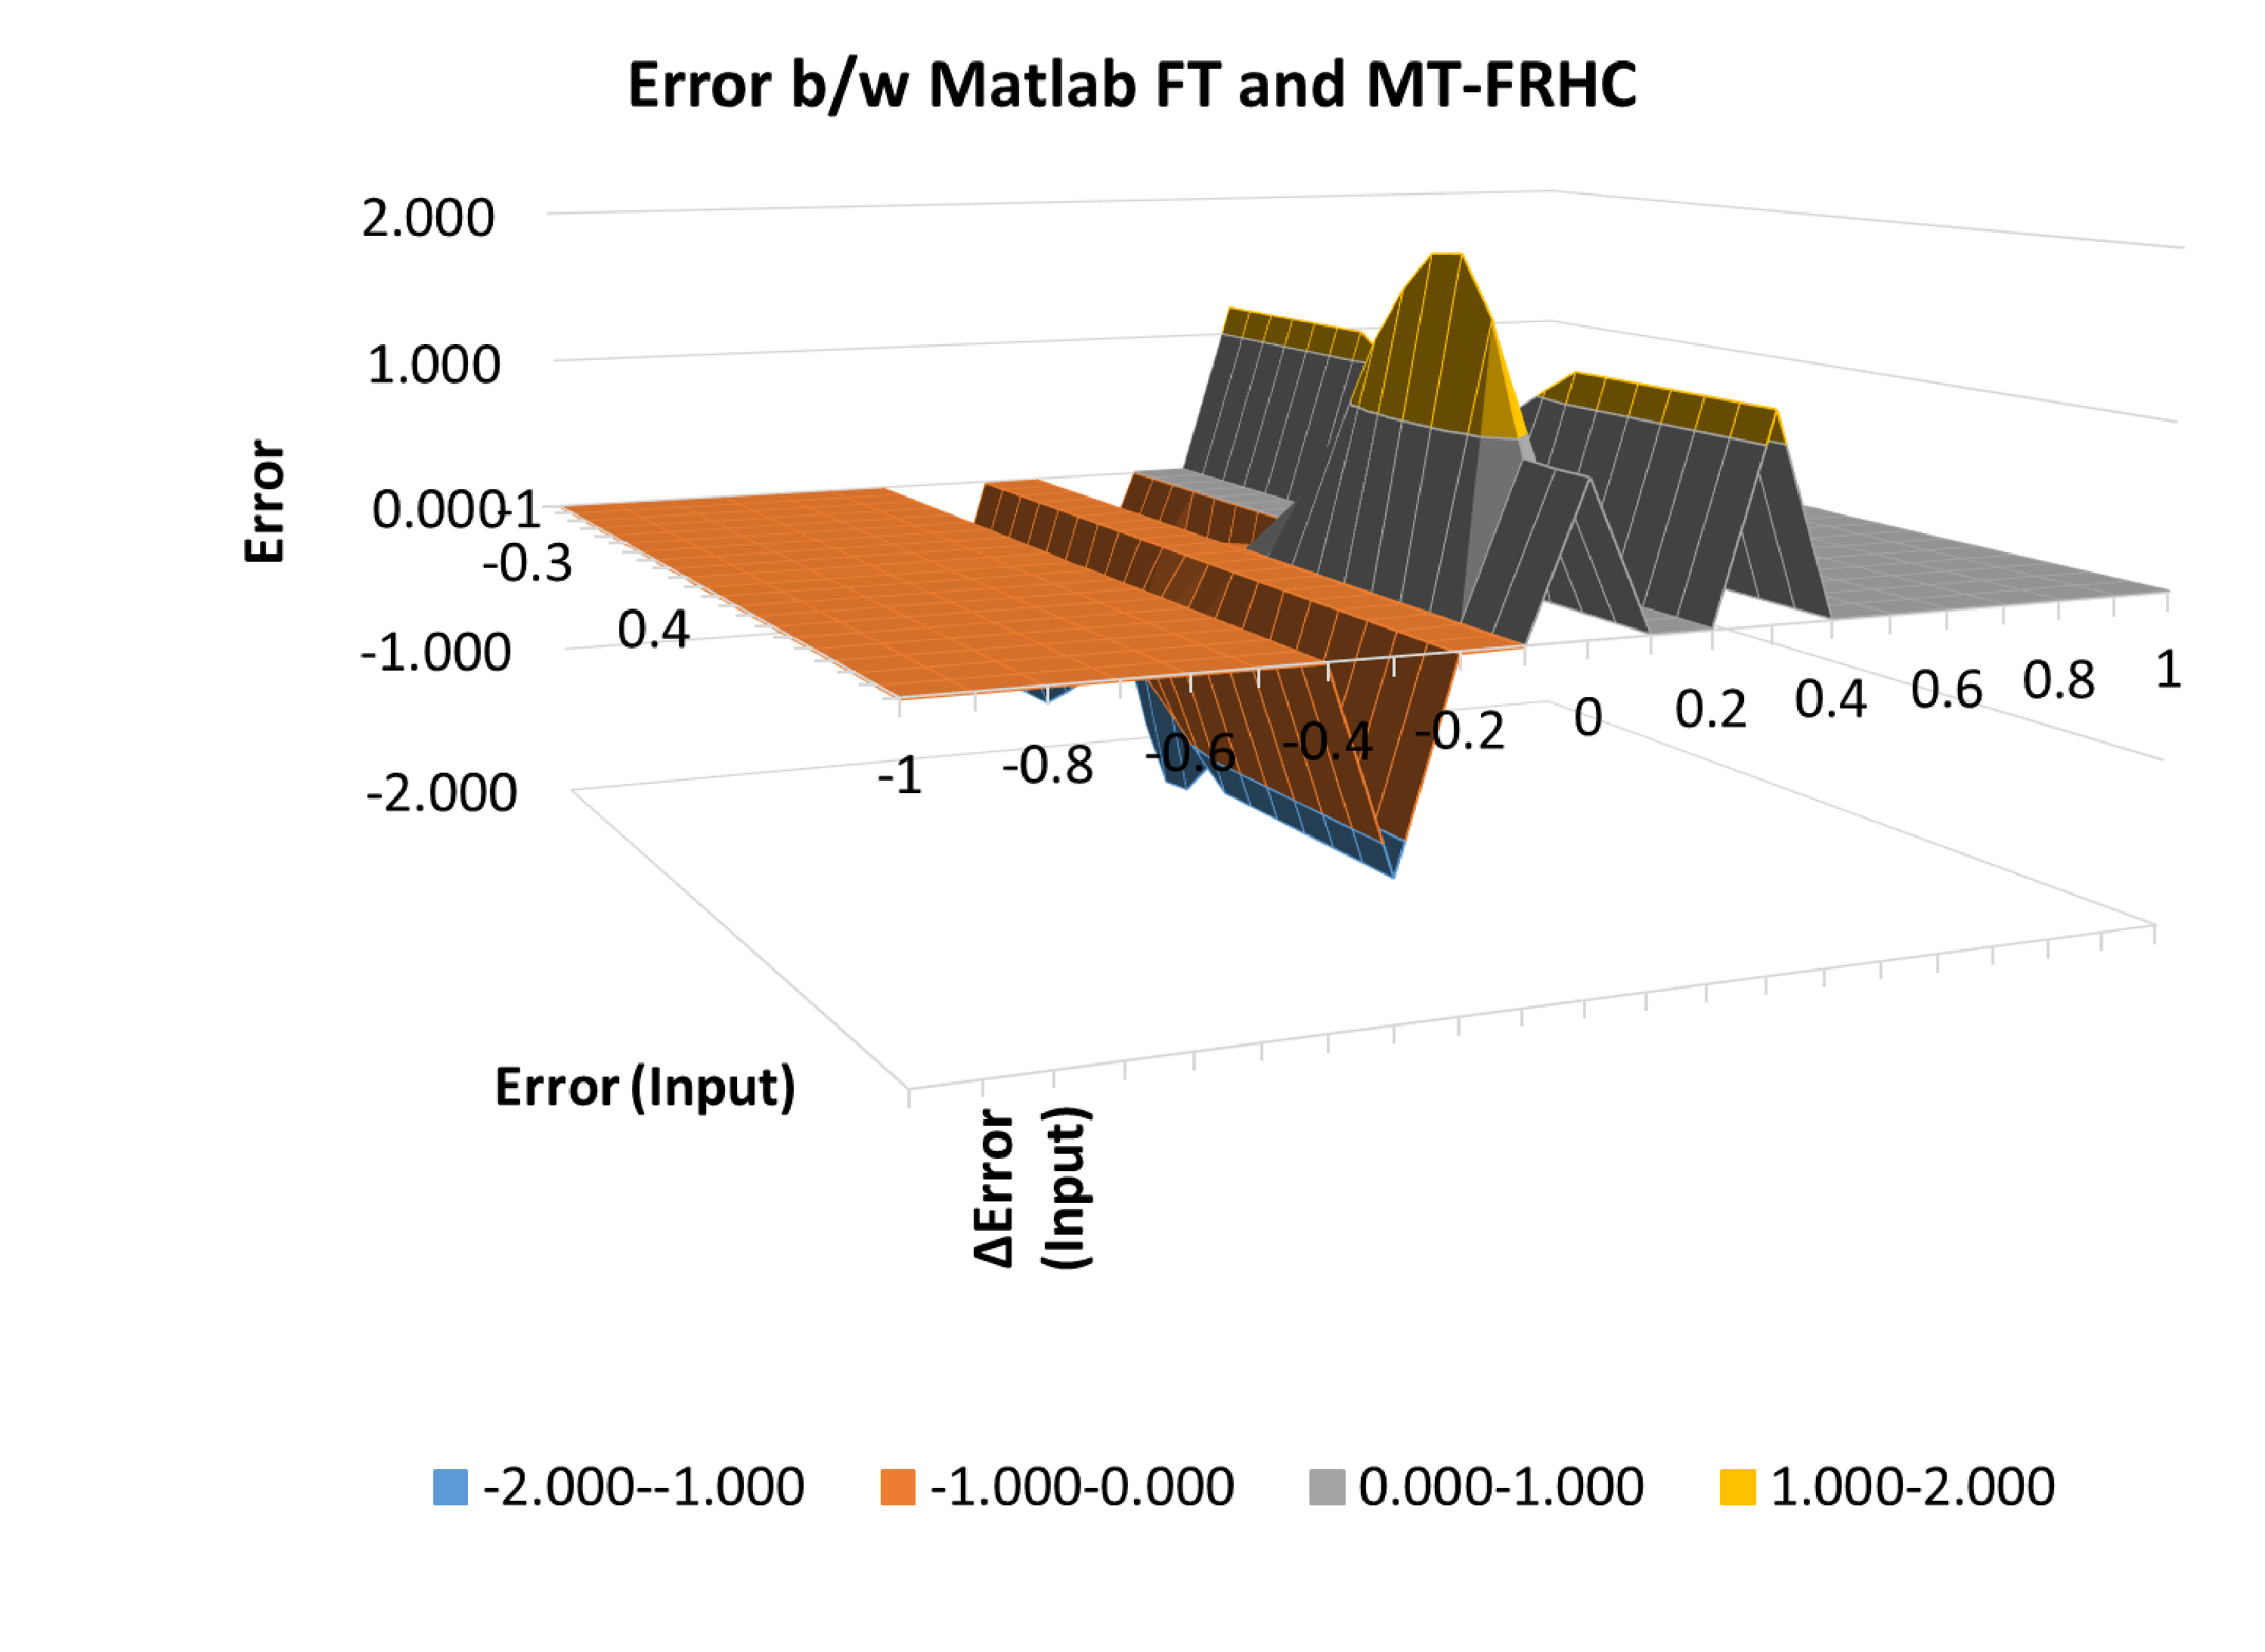
\includegraphics[width=0.6\linewidth]{Chapter2/chapter2/error_plot.eps}}
	\caption{Surface Plot to test Fuzzy Inference Parameter for Fuzzy Inference Structure (FIS) used in Fuzzy PI approximation controller for ACDC motor control \cite{malla2012}}
	\label{fig:SurfacePlot_ACDC}
\end{figure}

\begin{figure}[htbp]
	\centering
	\subfloat[Two Tank FIS: MT-FRHC]{\label{fig:SPlot_MT-FRHC_tank}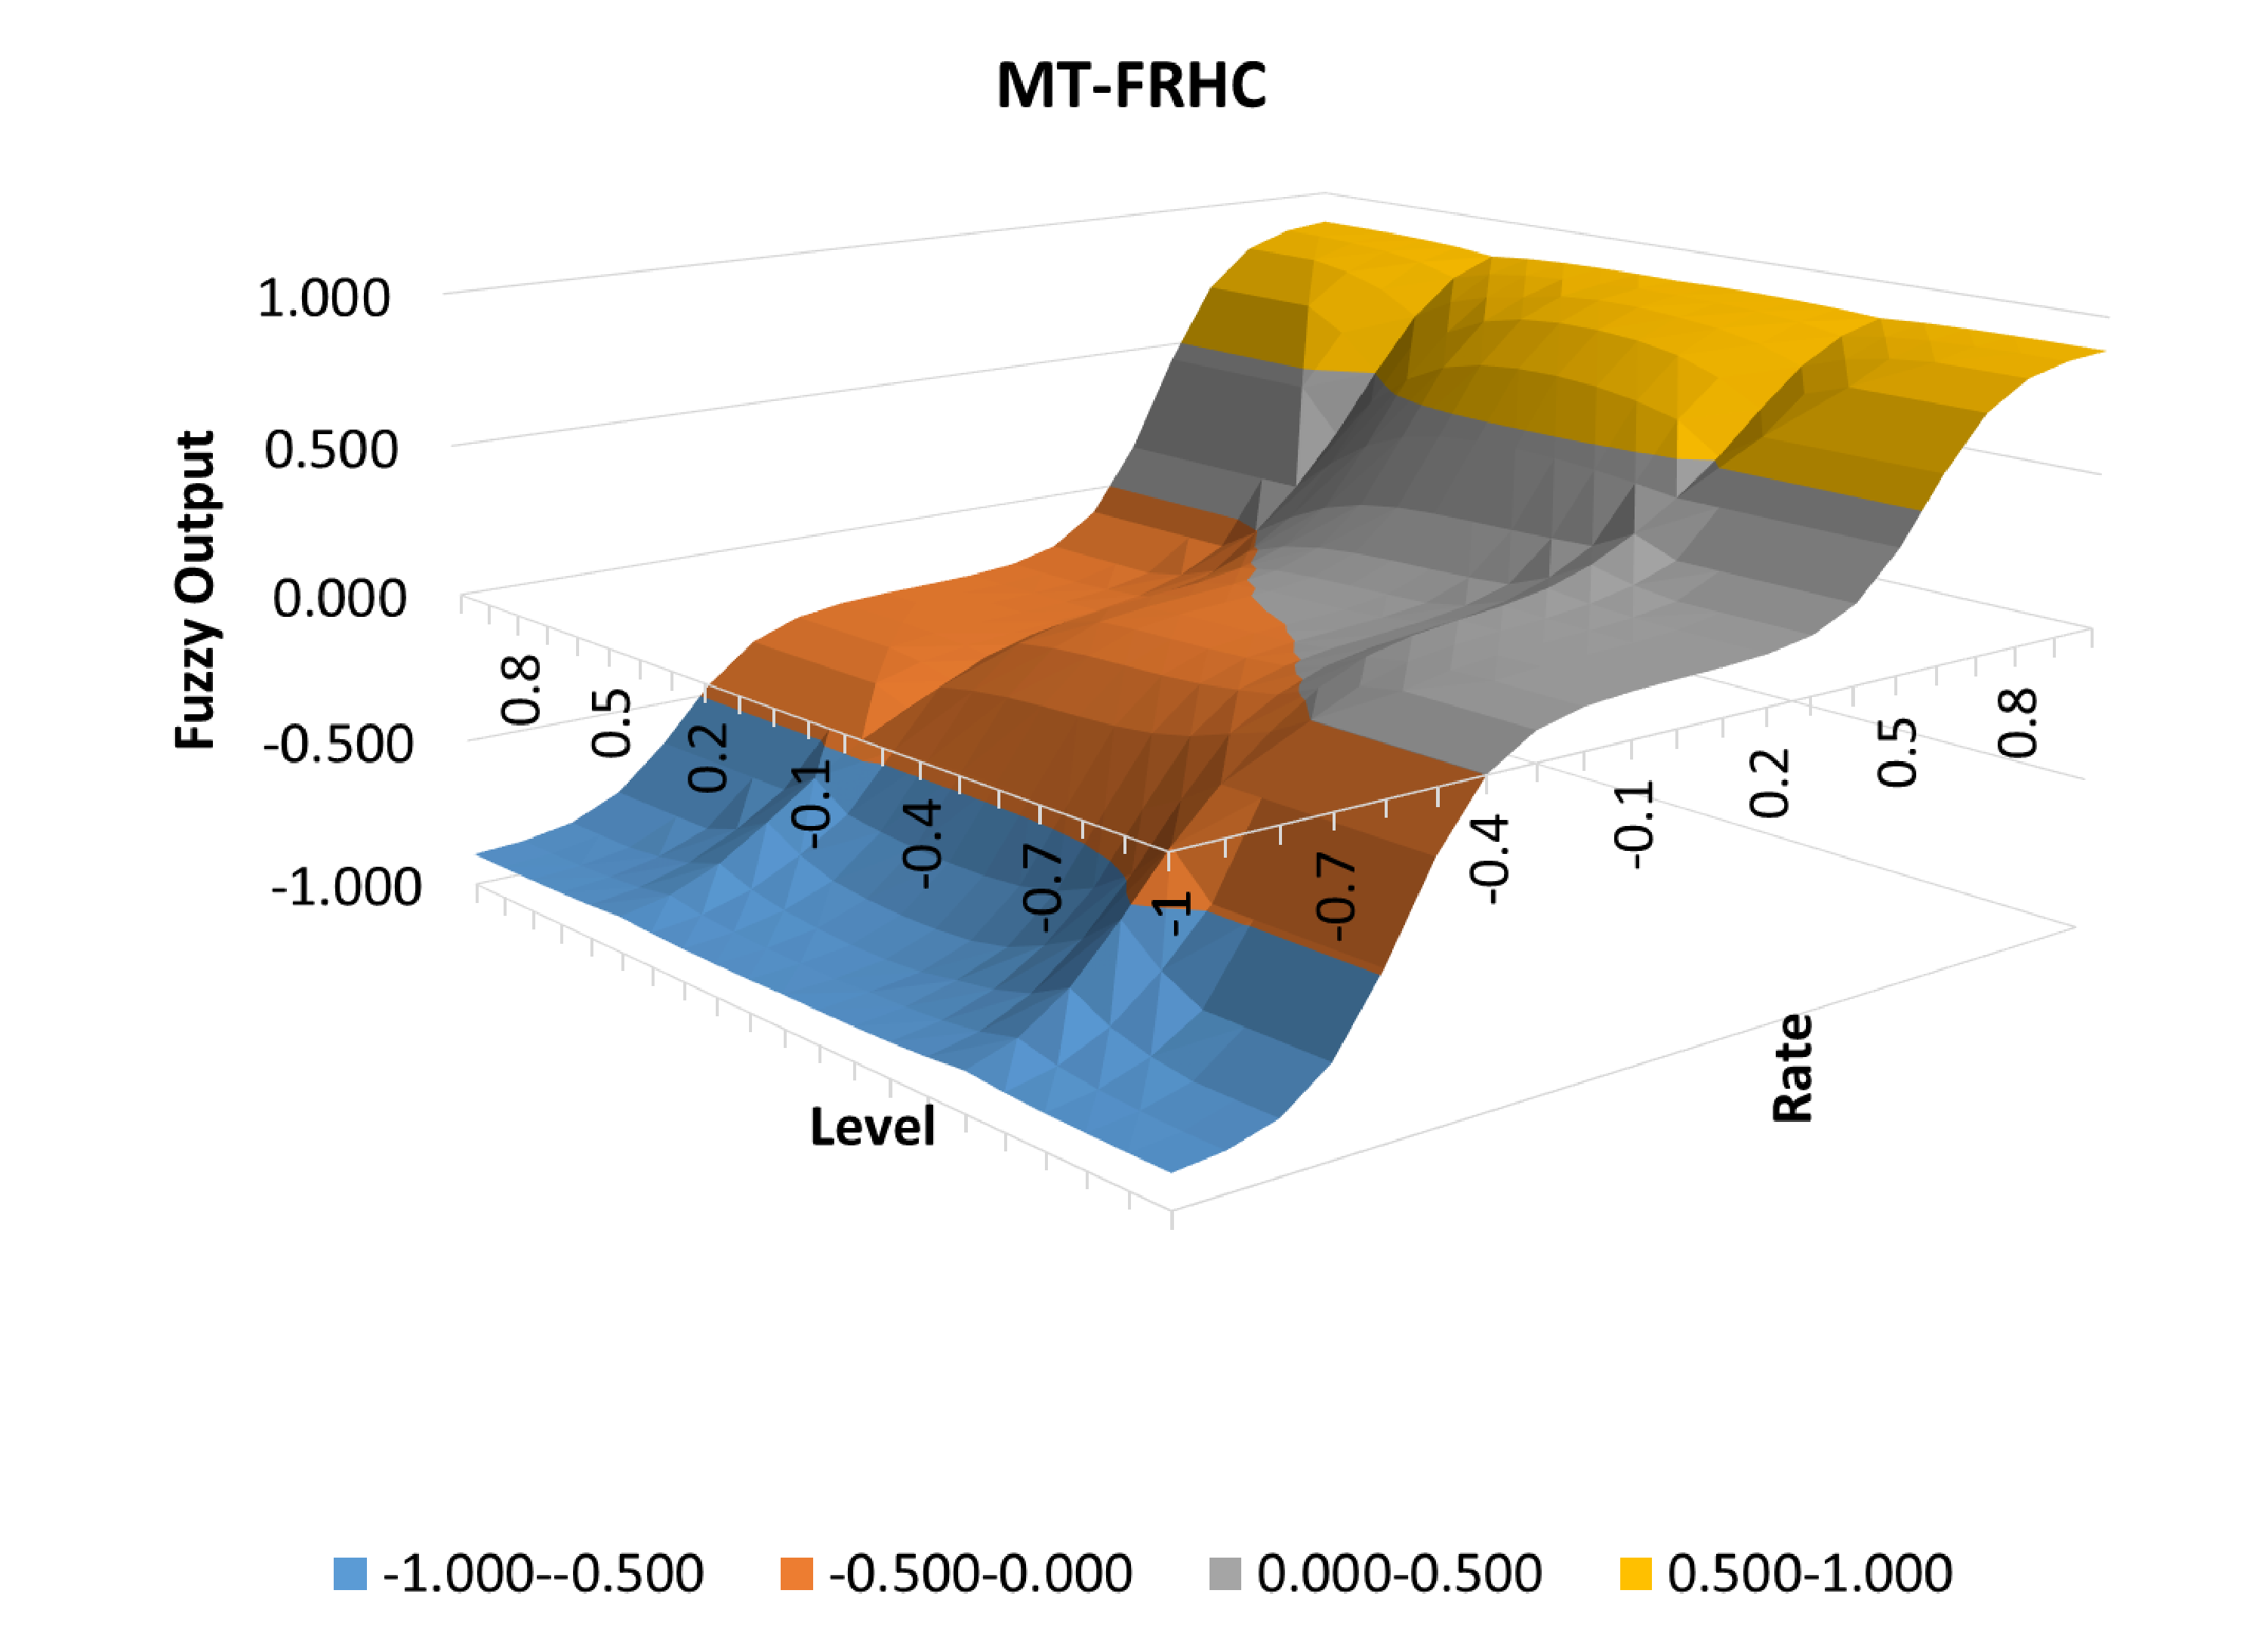
\includegraphics[width=0.6\linewidth]{Chapter2/chapter2/tank_MTFRHC.eps}} \\
	\subfloat[Two Tank FIS: Matlab Fuzzy Toolbox]{\label{fig:SPlot_MFT_tank}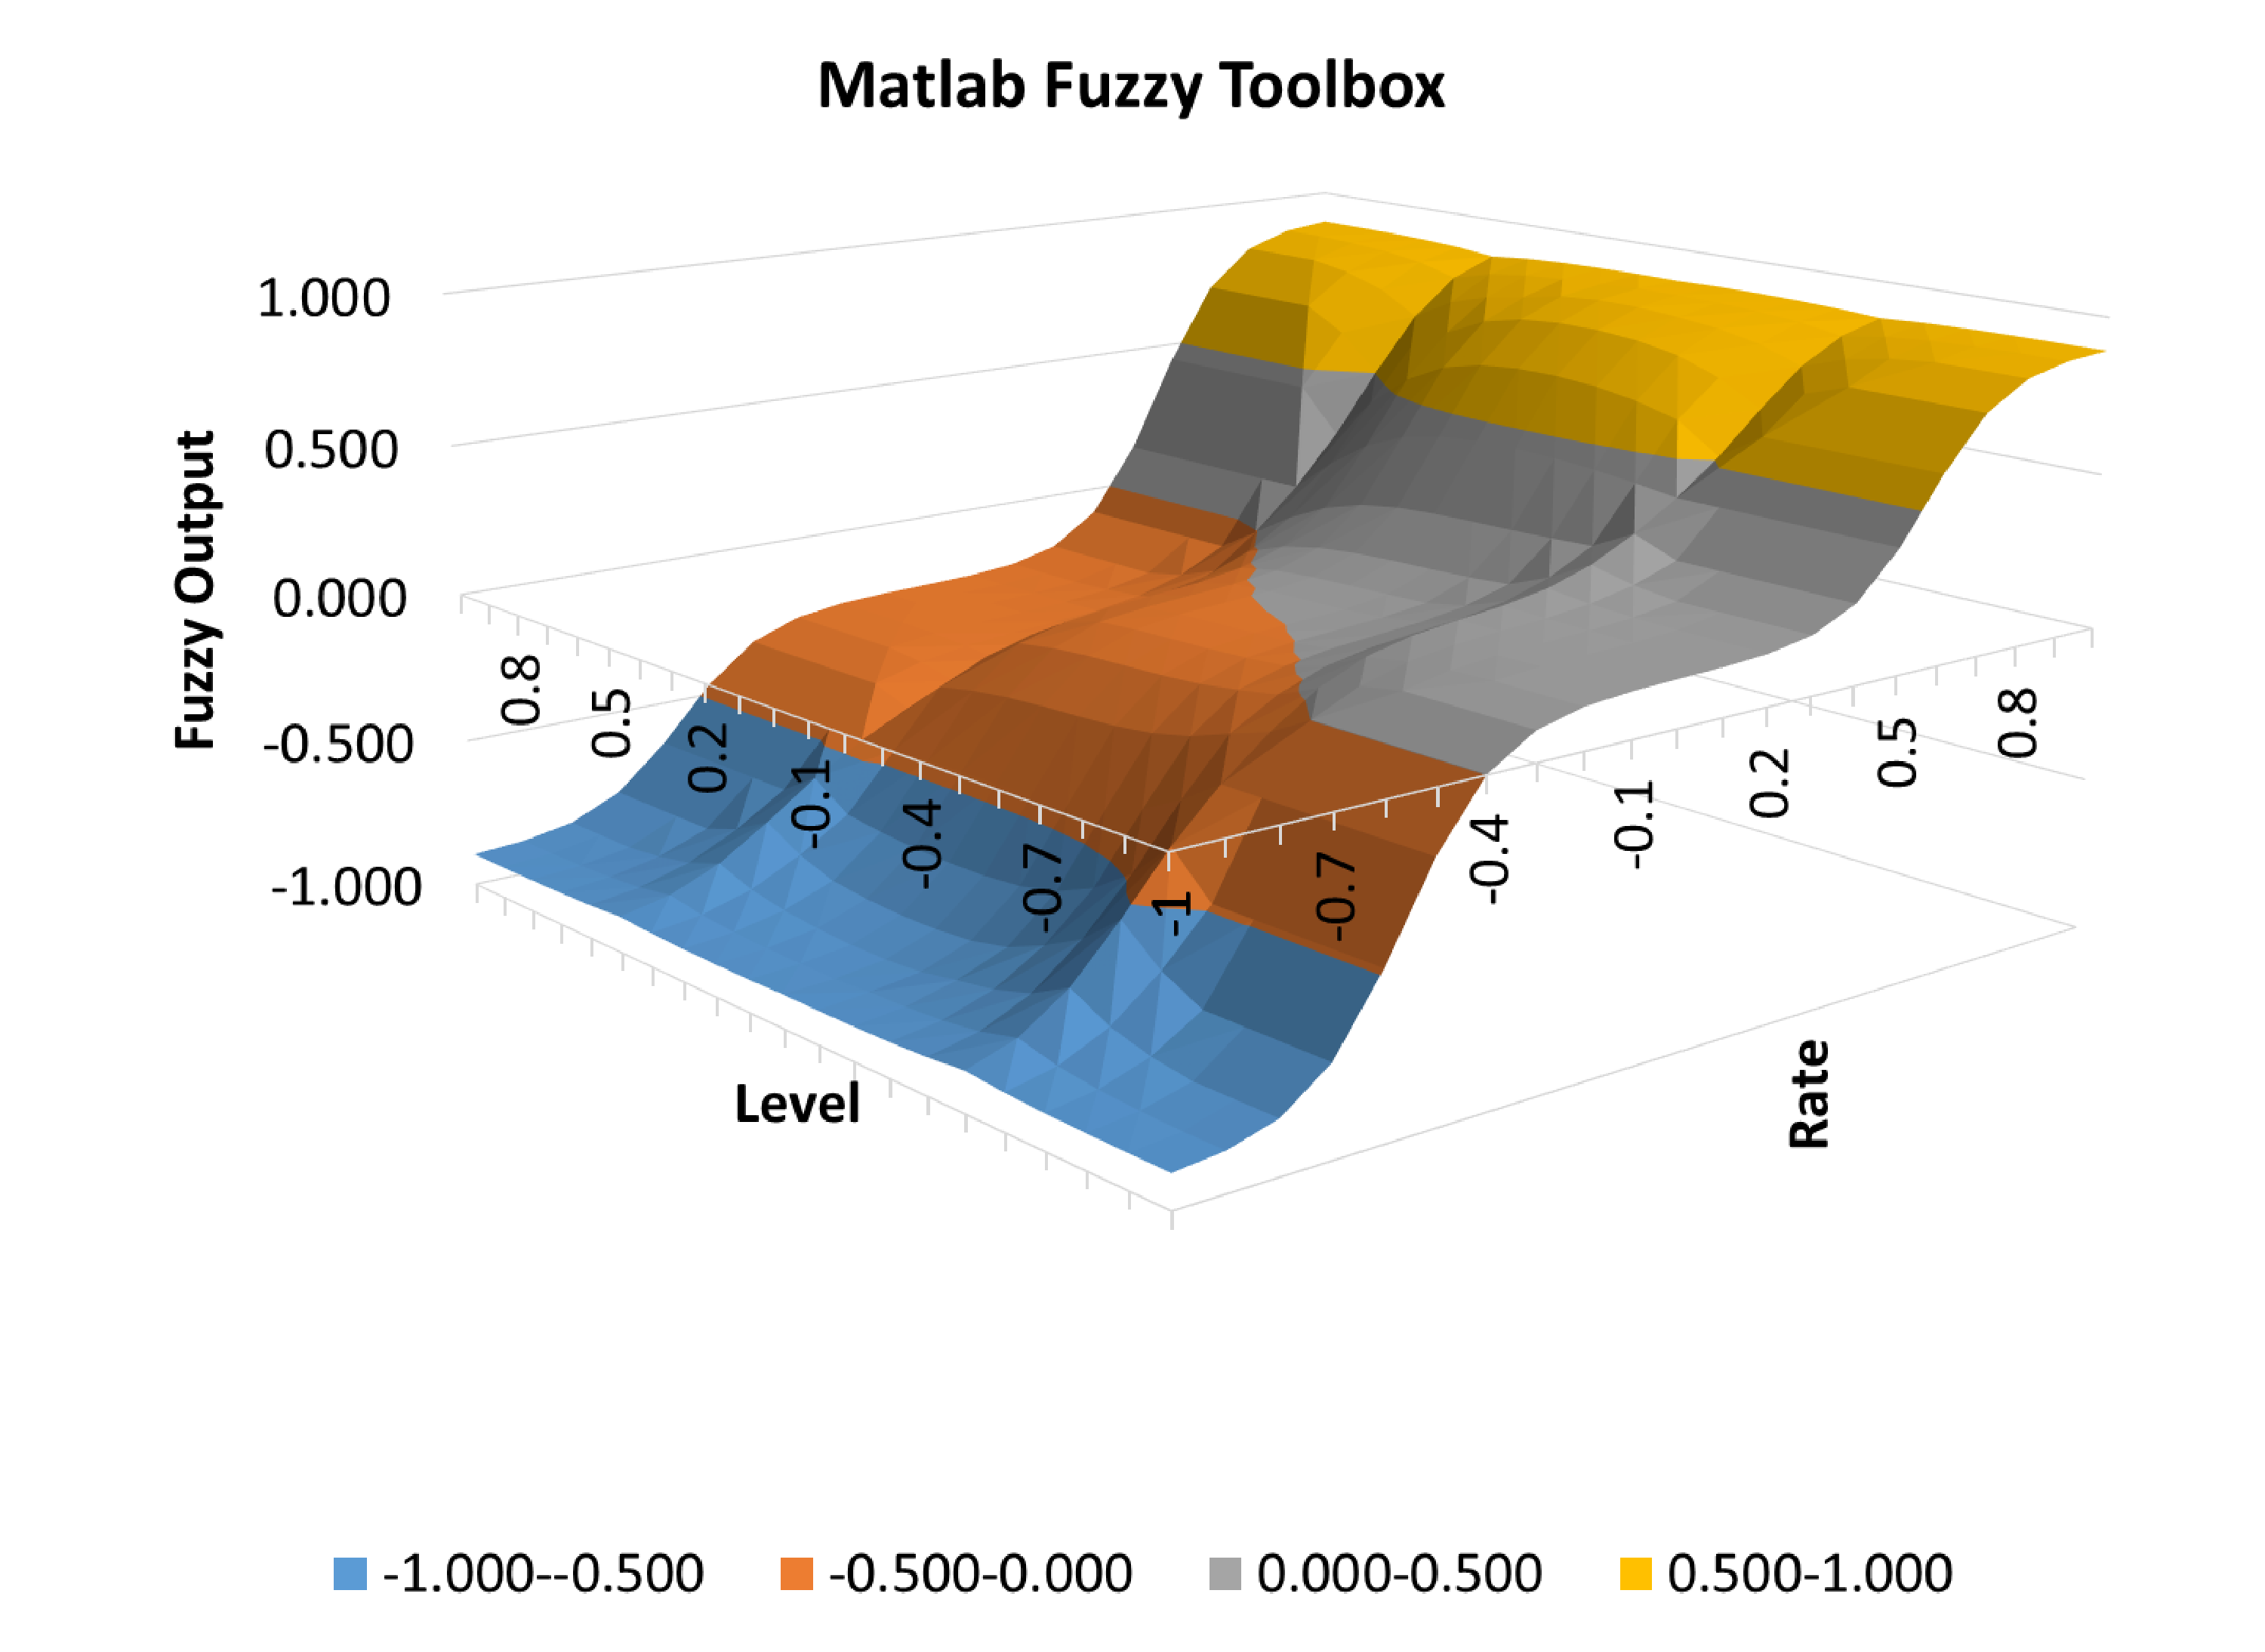
\includegraphics[width=0.6\linewidth]{Chapter2/chapter2/tank_MFT.eps}} \\
	\subfloat[Two Tank FIS: Error Plot]{\label{fig:SPlot_Error_tank}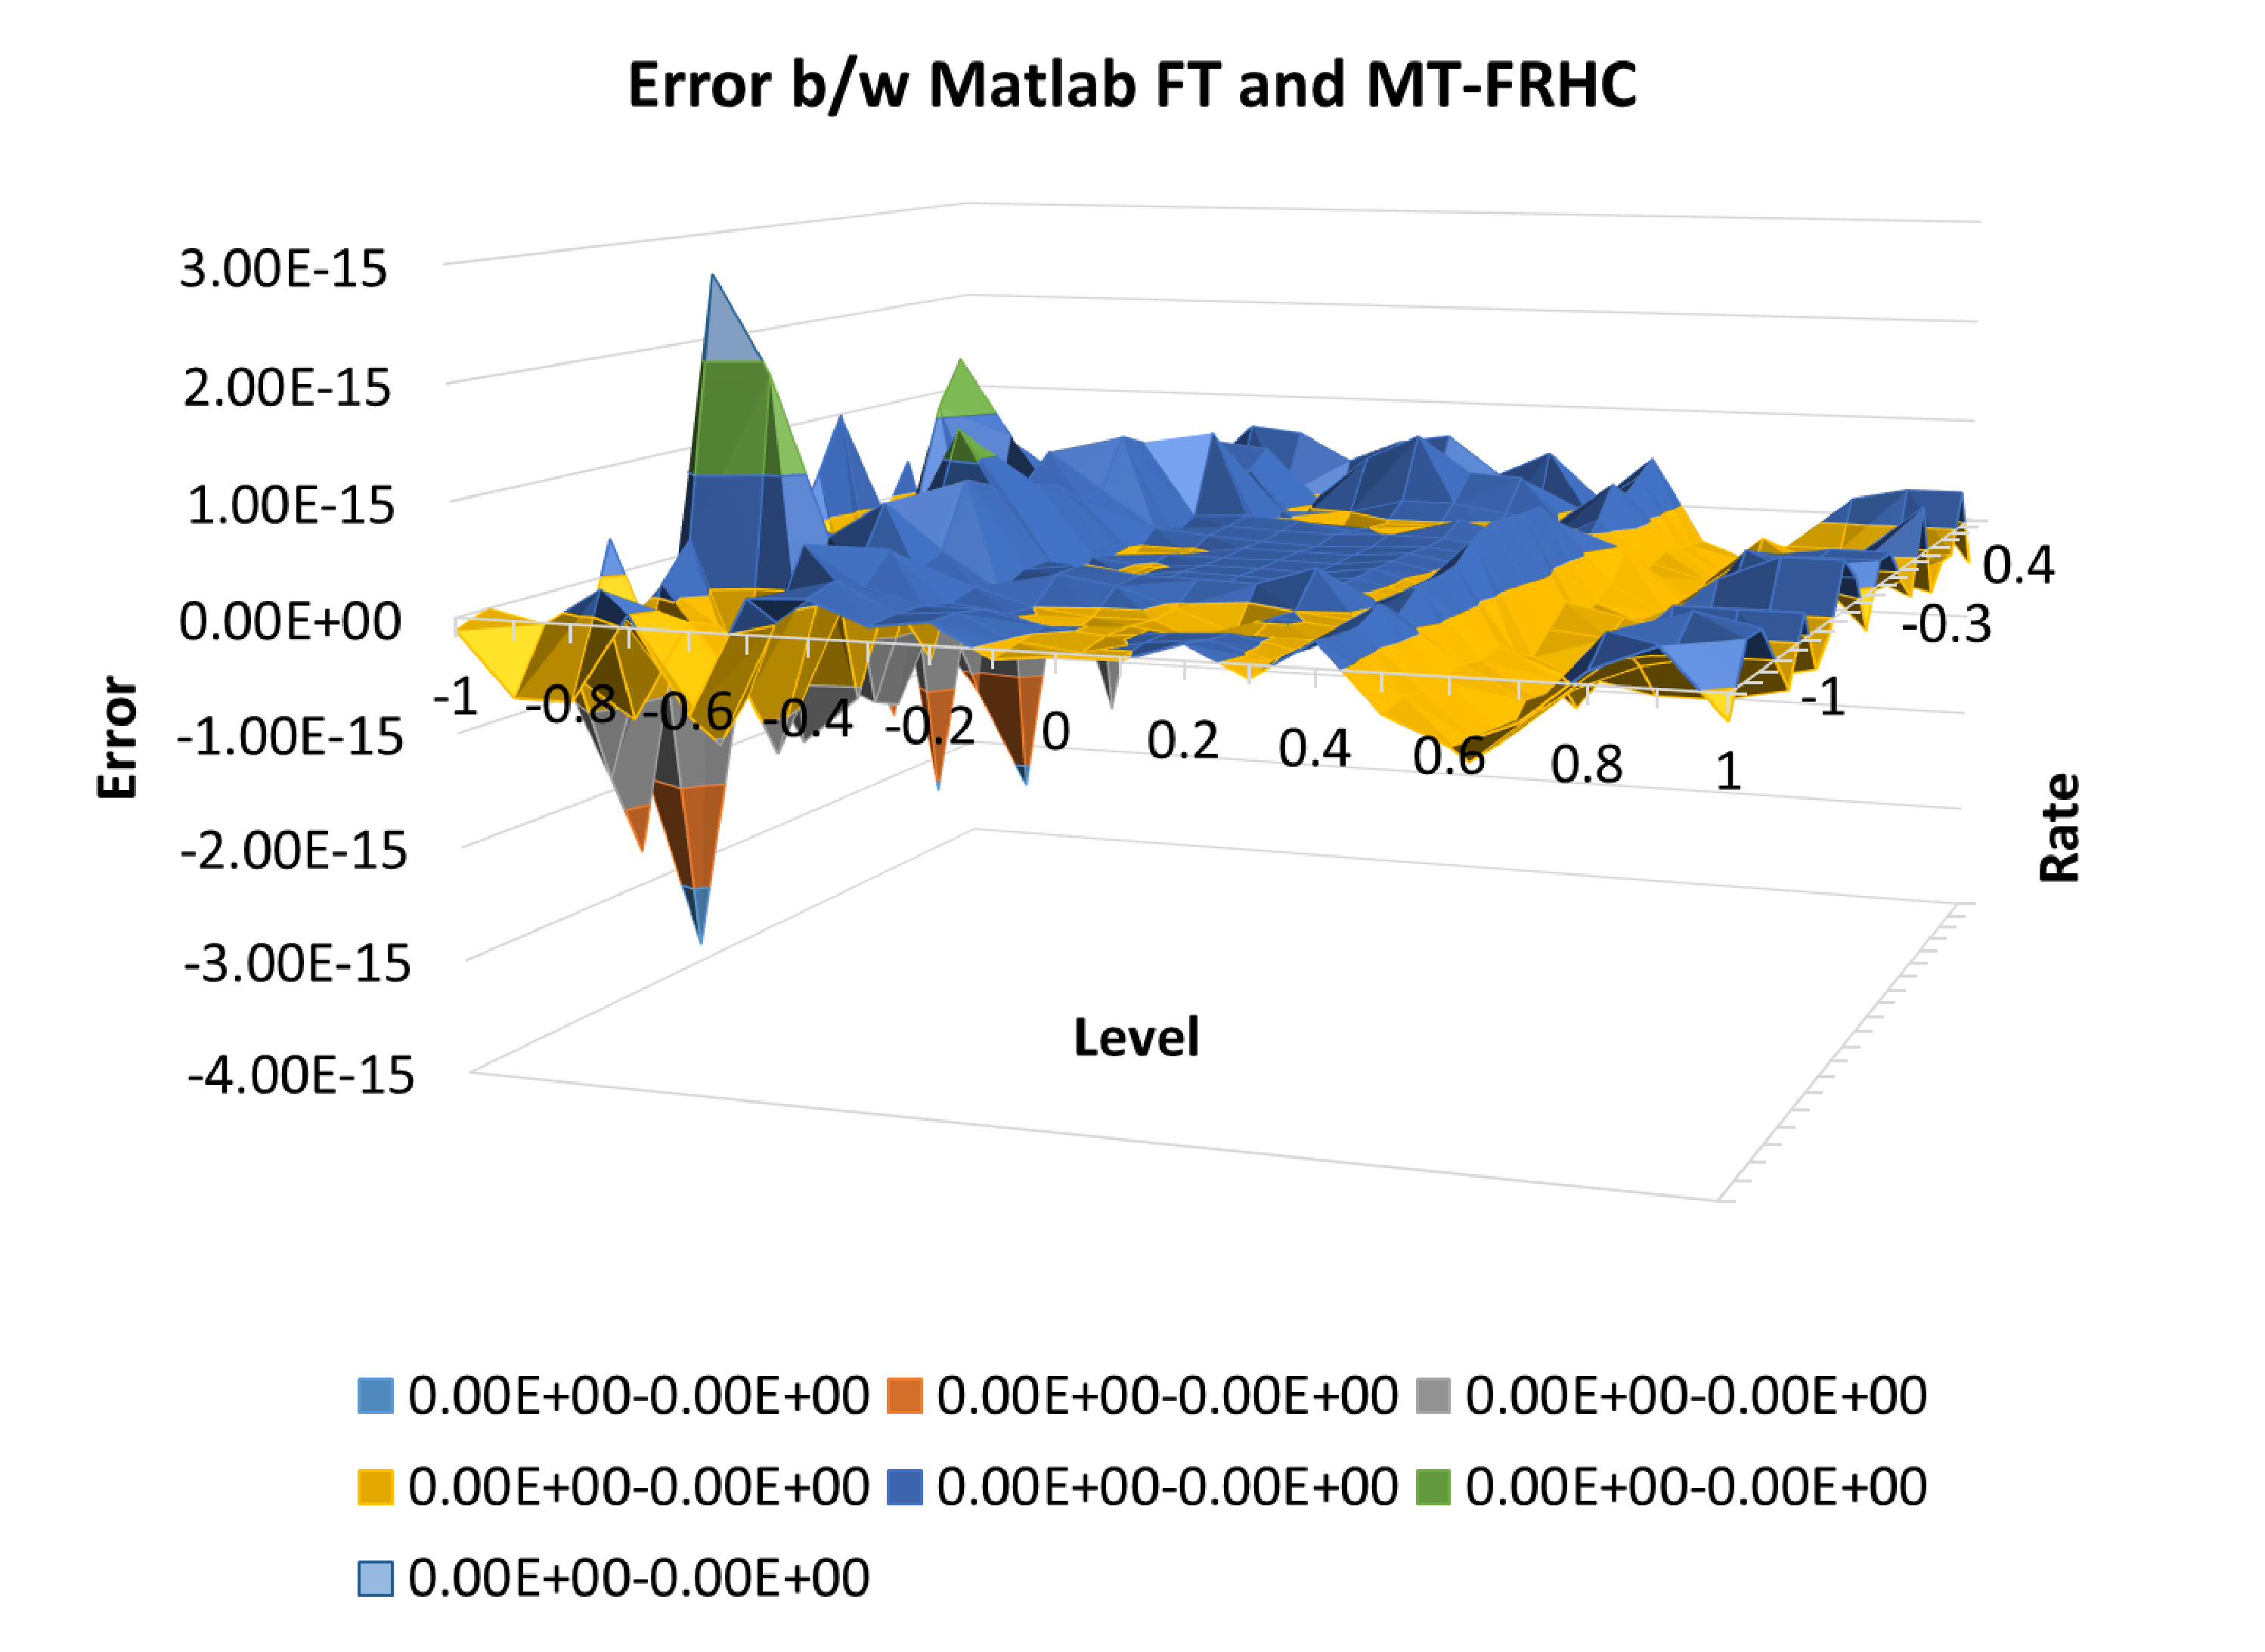
\includegraphics[width=0.6\linewidth]{Chapter2/chapter2/tank_Error.eps}}
	\caption{Surface Plot to test Fuzzy Inference Parameter for Fuzzy Inference Structure (FIS) used in Fuzzy PI approximation controller for Two Tank System \cite{twotank2012}}
	\label{fig:SurfacePlot_tank}
\end{figure}

\begin{figure}[htbp] 
	\centering
	\subfloat[Truck Backer FIS: MT-FRHC]{\label{fig:SPlot_MT-FRHC_truck}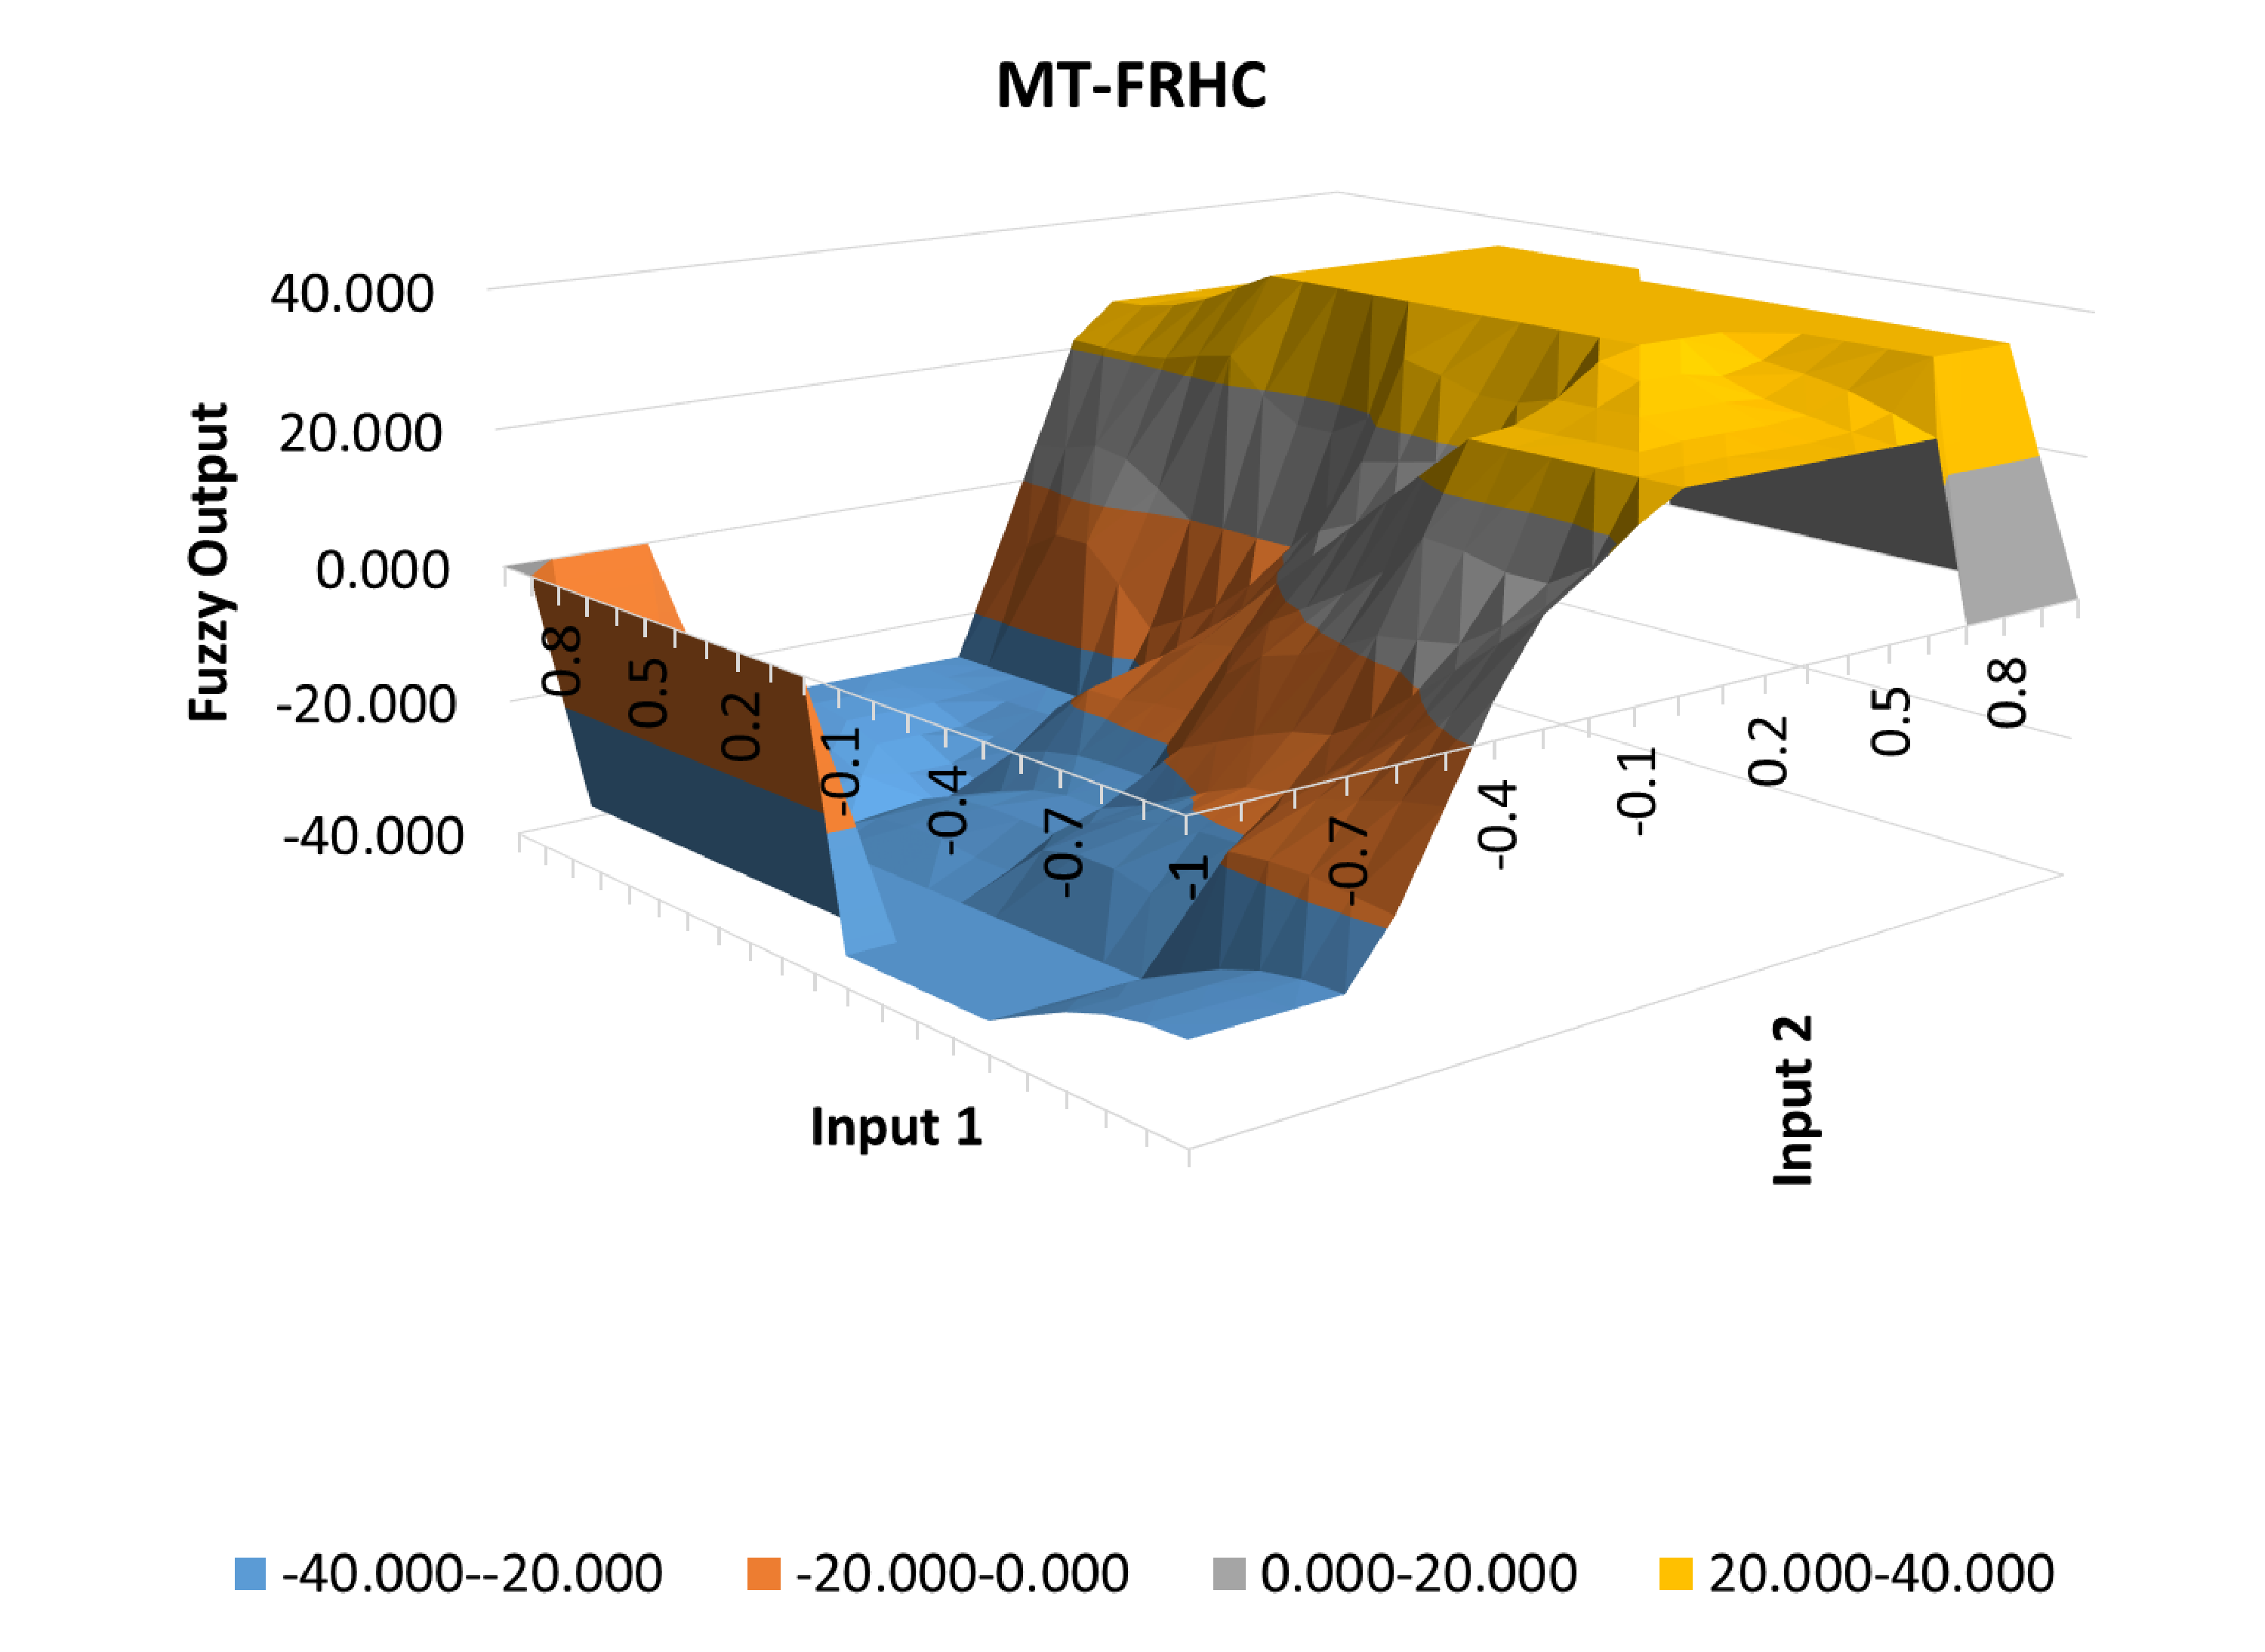
\includegraphics[width=0.6\linewidth]{Chapter2/chapter2/truck_MTFRHC.eps}} \\
	\subfloat[Truck Backer FIS: Matlab Fuzzy Toolbox]{\label{fig:SPlot_MFT_truck}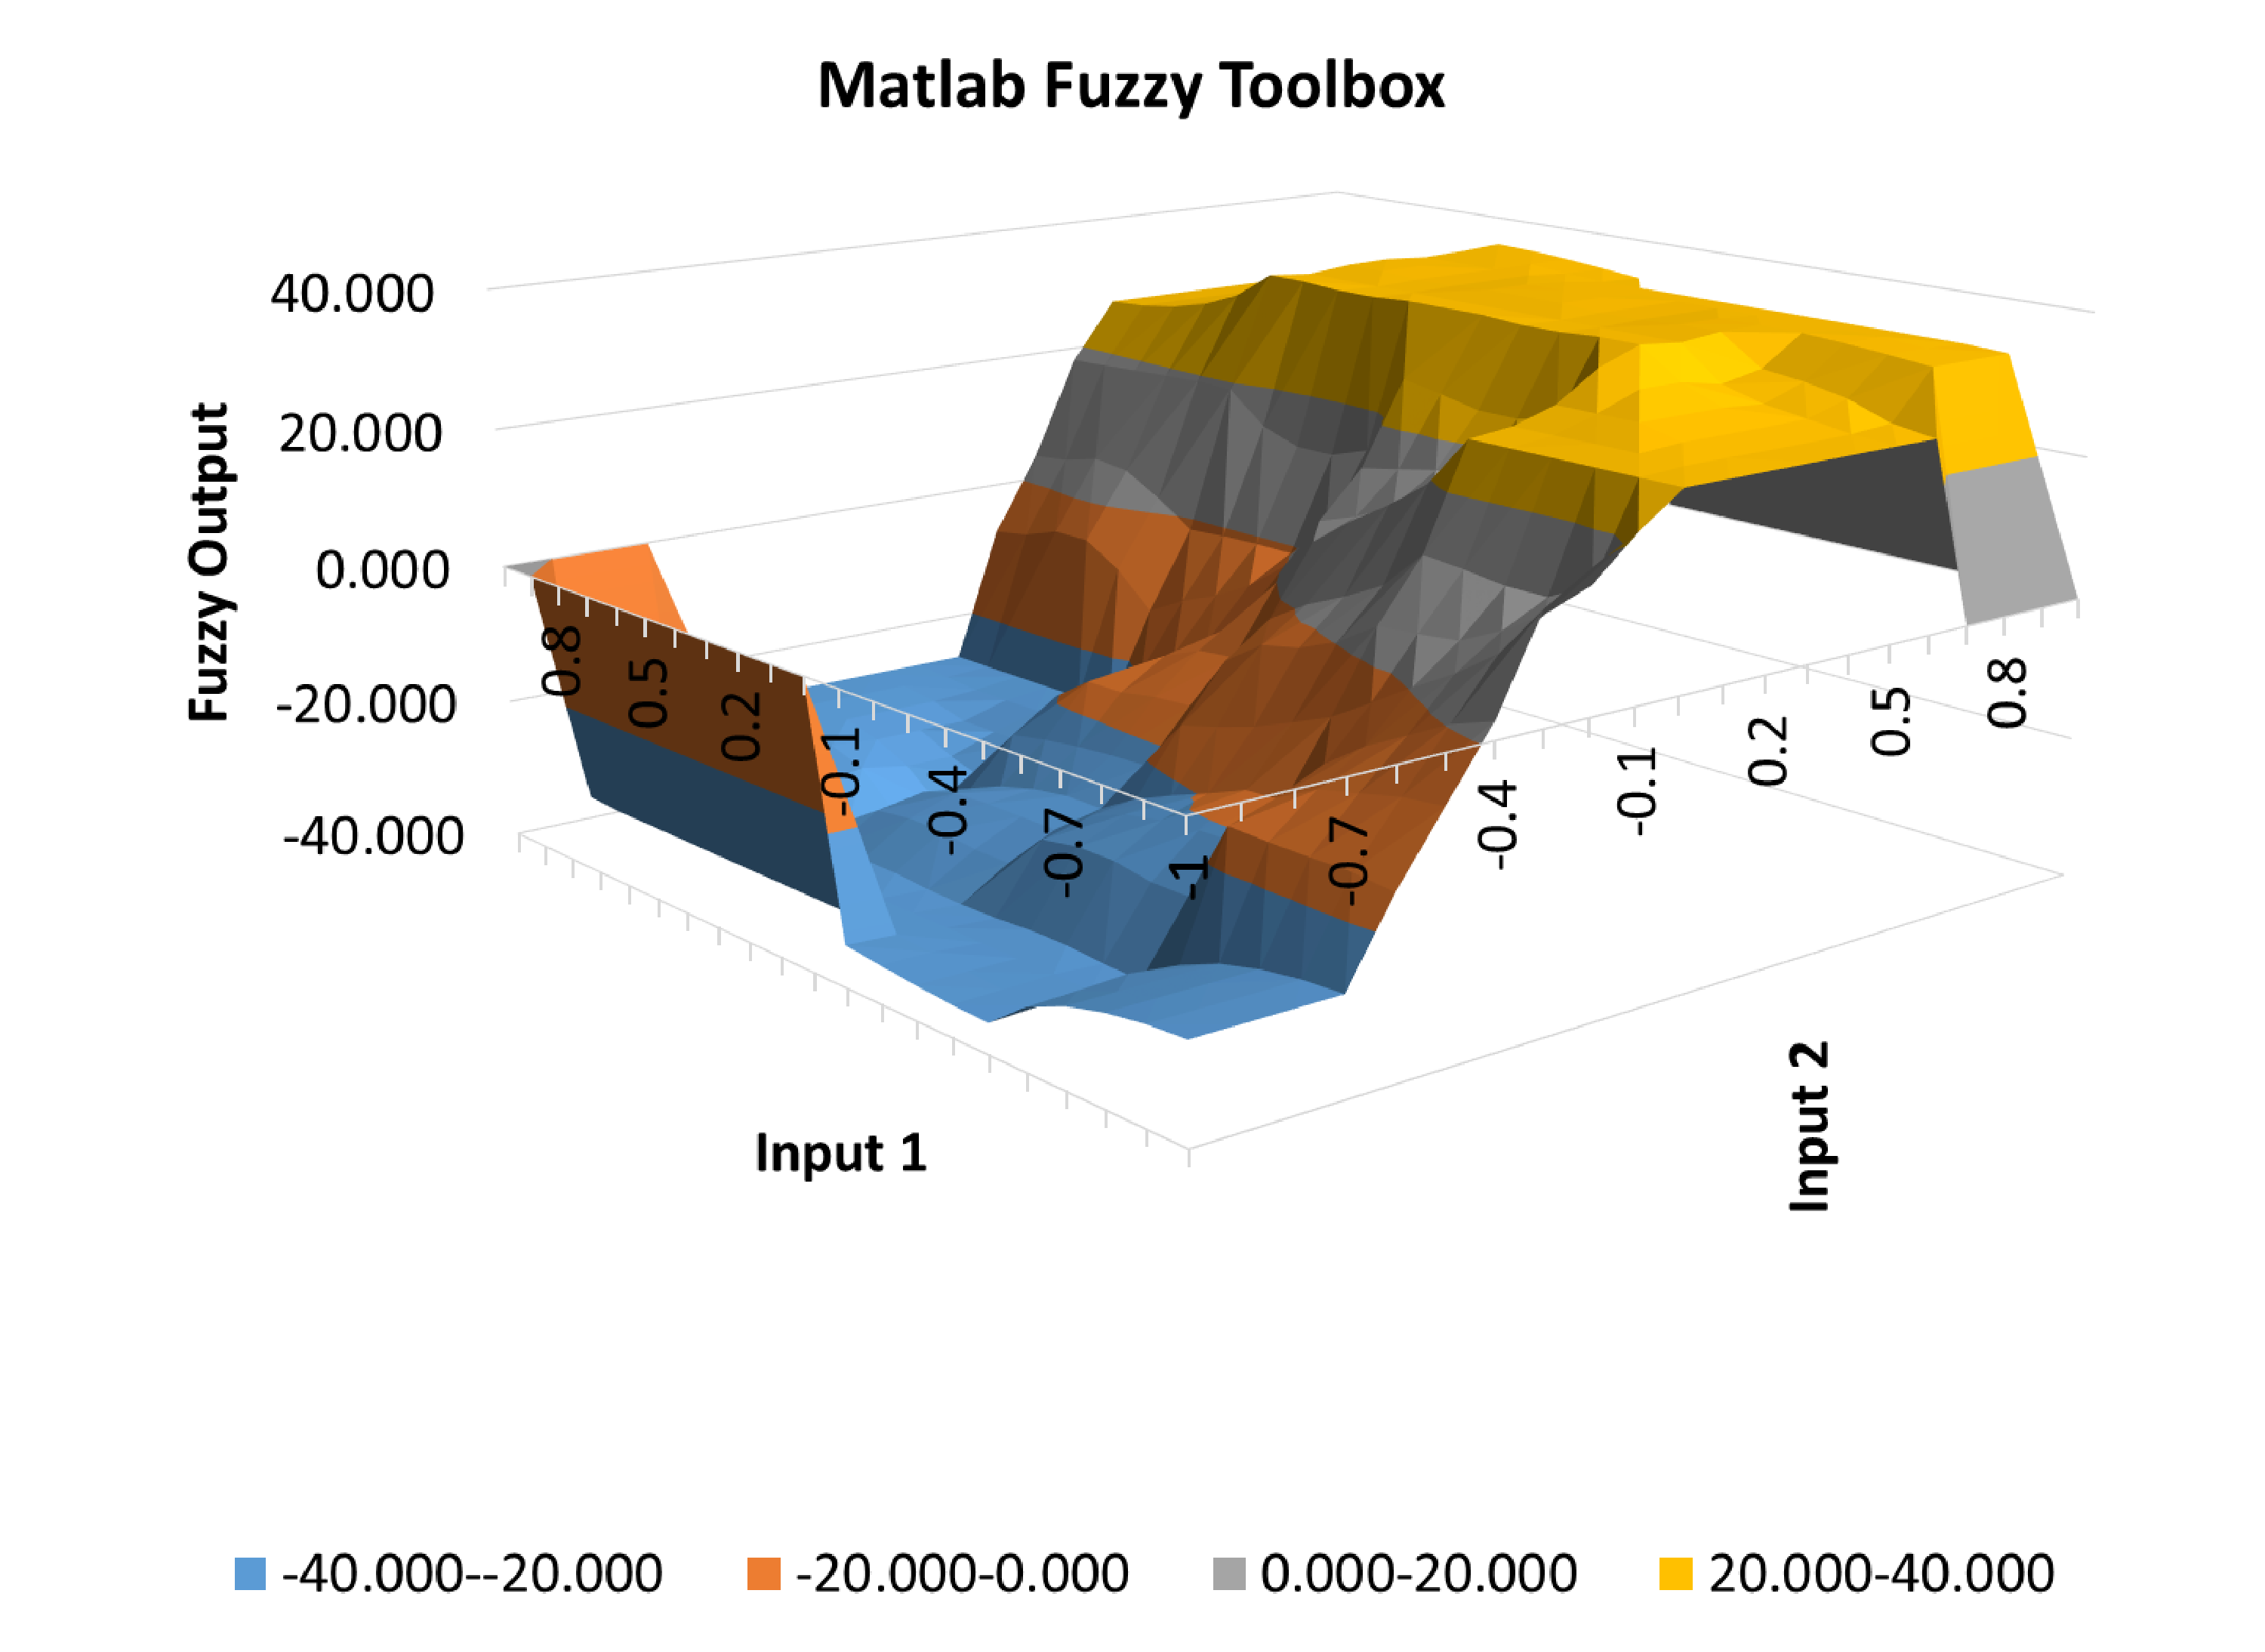
\includegraphics[width=0.6\linewidth]{Chapter2/chapter2/truck_MFT.eps}} \\ 
	\subfloat[Truck Backer FIS: Error Plot]{\label{fig:SPlot_Error_truck}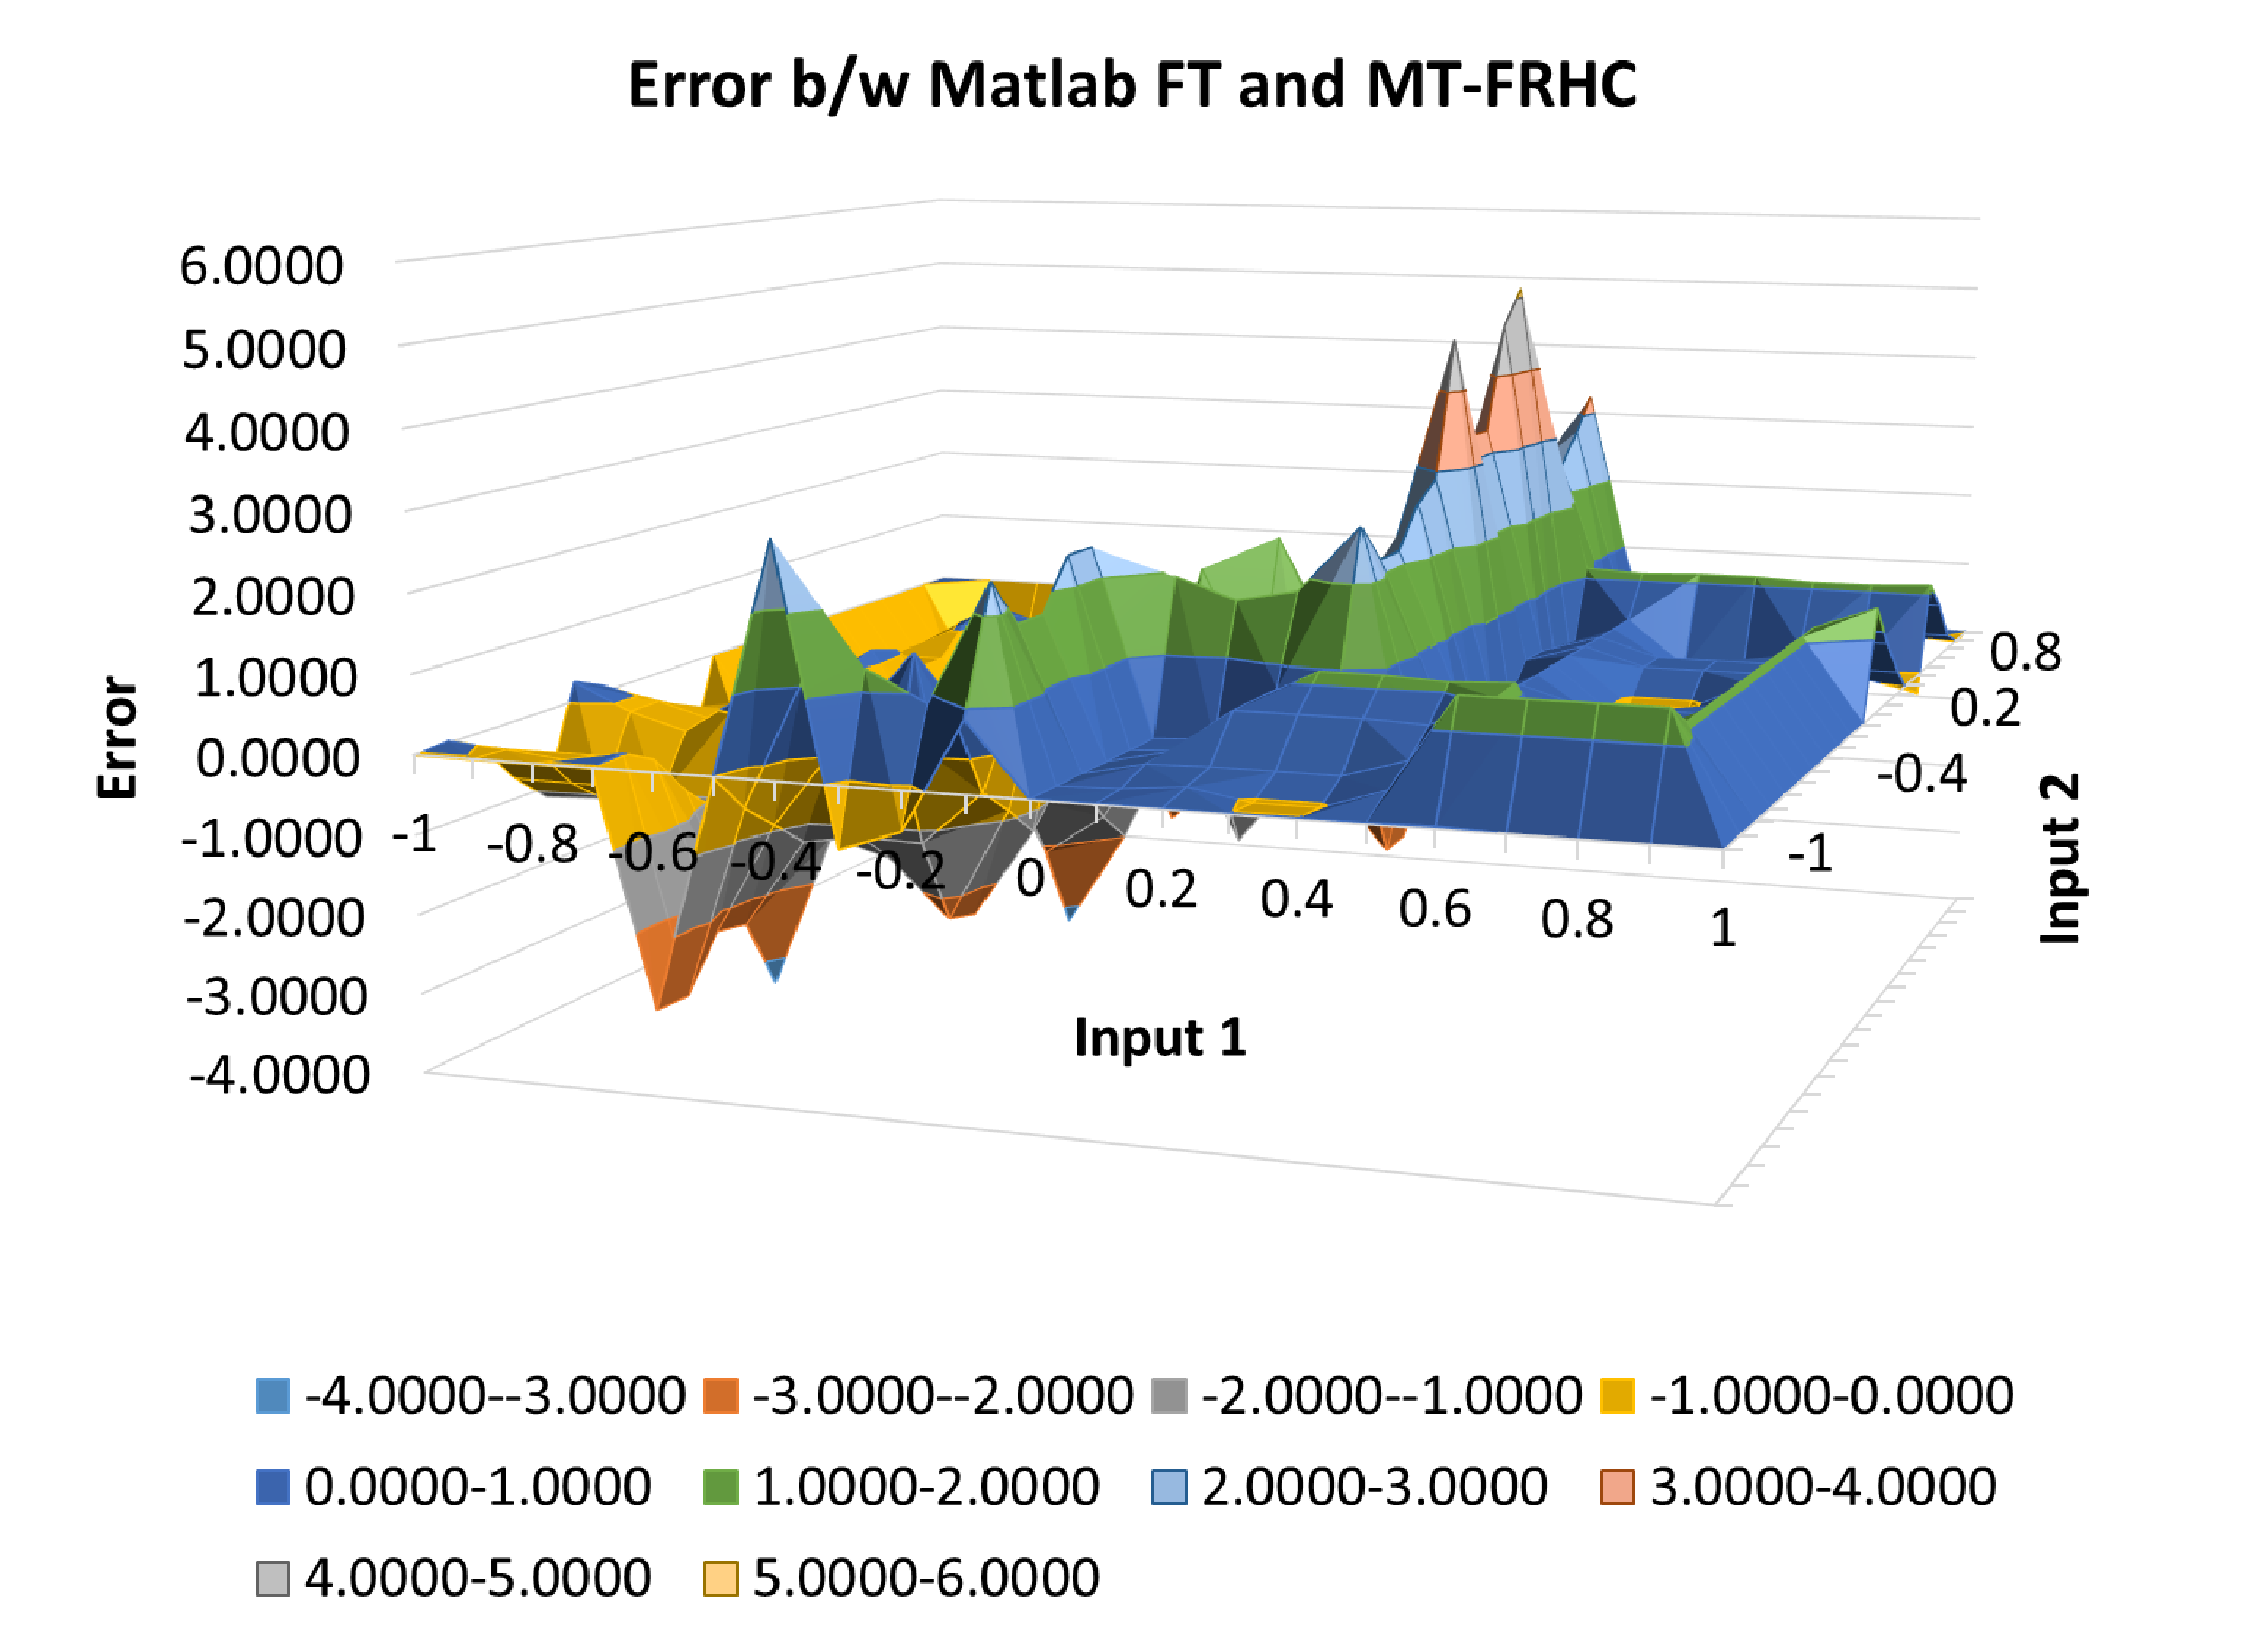
\includegraphics[width=0.6\linewidth]{Chapter2/chapter2/truck_Error.eps}}
	\caption{Surface Plot to test Fuzzy Inference Parameter for Fuzzy Inference Structure (FIS) used in Fuzzy PI approximation controller for Truck Backer Control \cite{Passino2010} }
	\label{fig:SurfacePlot_truck}
\end{figure}

\begin{figure}[h!]
	\centering
	\subfloat[Fuzzy PI Approximation to Control ACDC Motor]{\label{fig:MSEvTH_ACDC}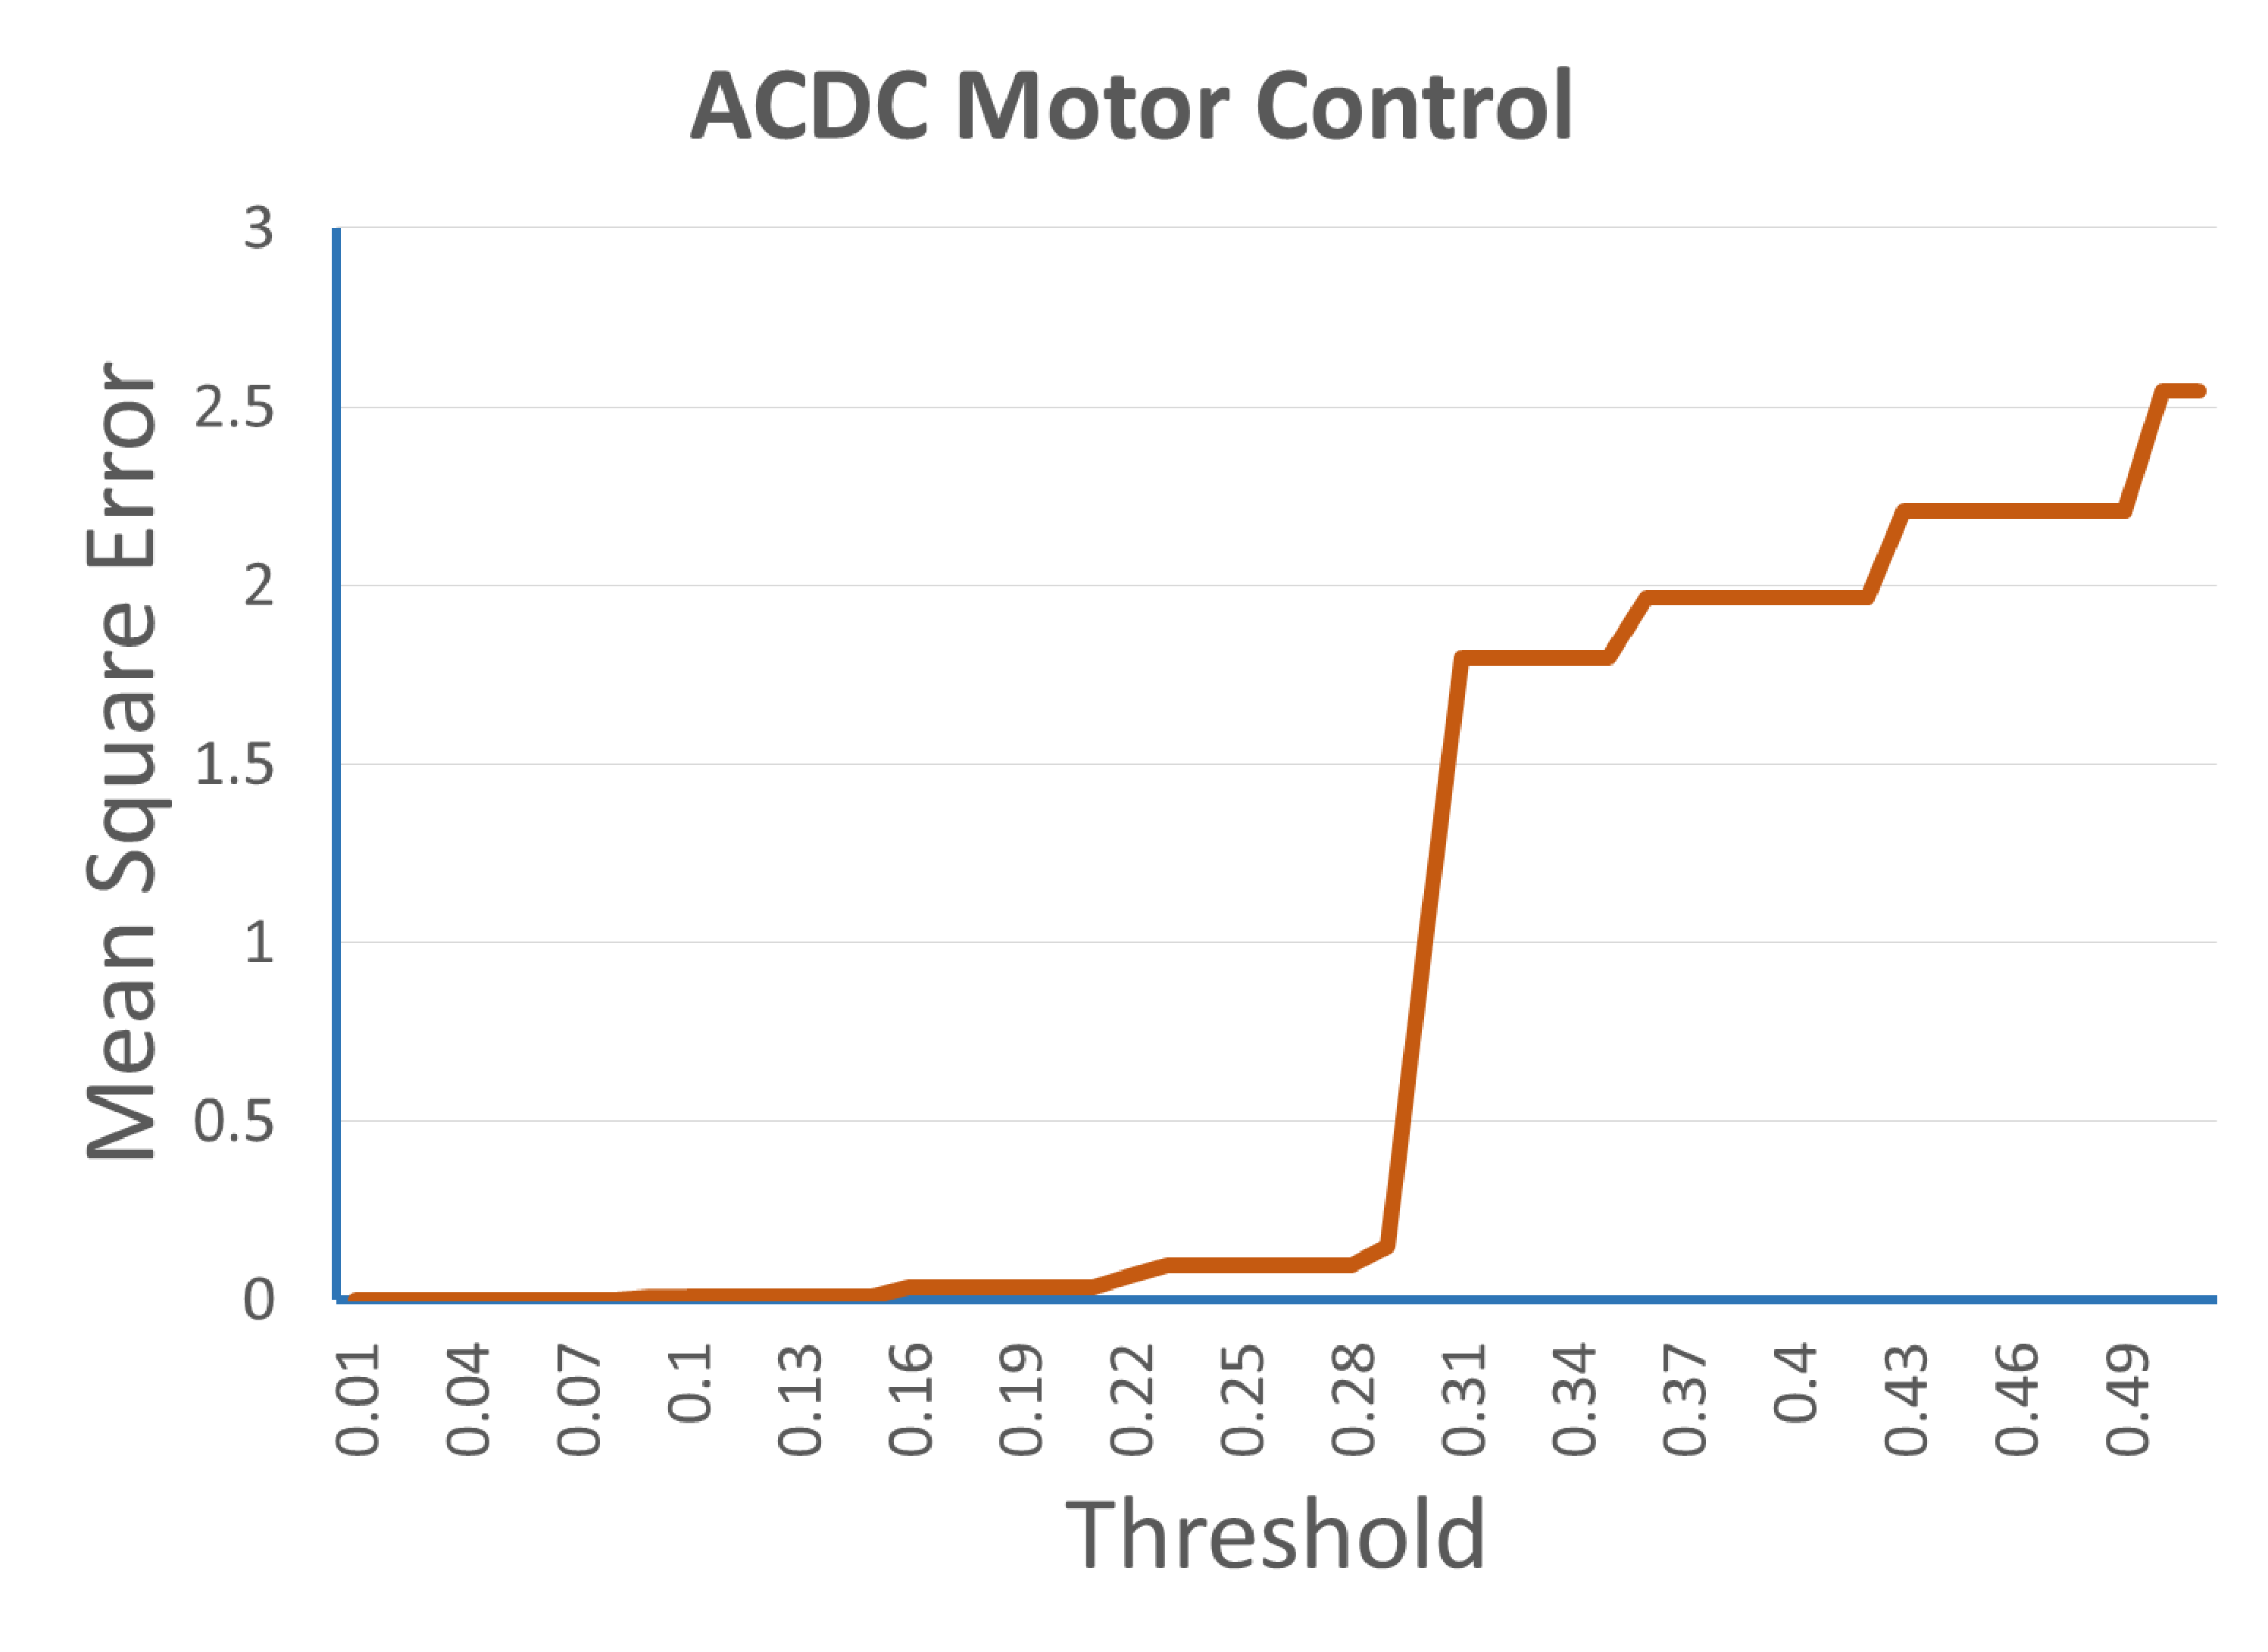
\includegraphics[width=0.55\linewidth]{Chapter2/chapter2/MSEvTH_ACDC}}\\
	\subfloat[Water Level Control of Two Tank System]{\label{fig:MSEvTH_Tank}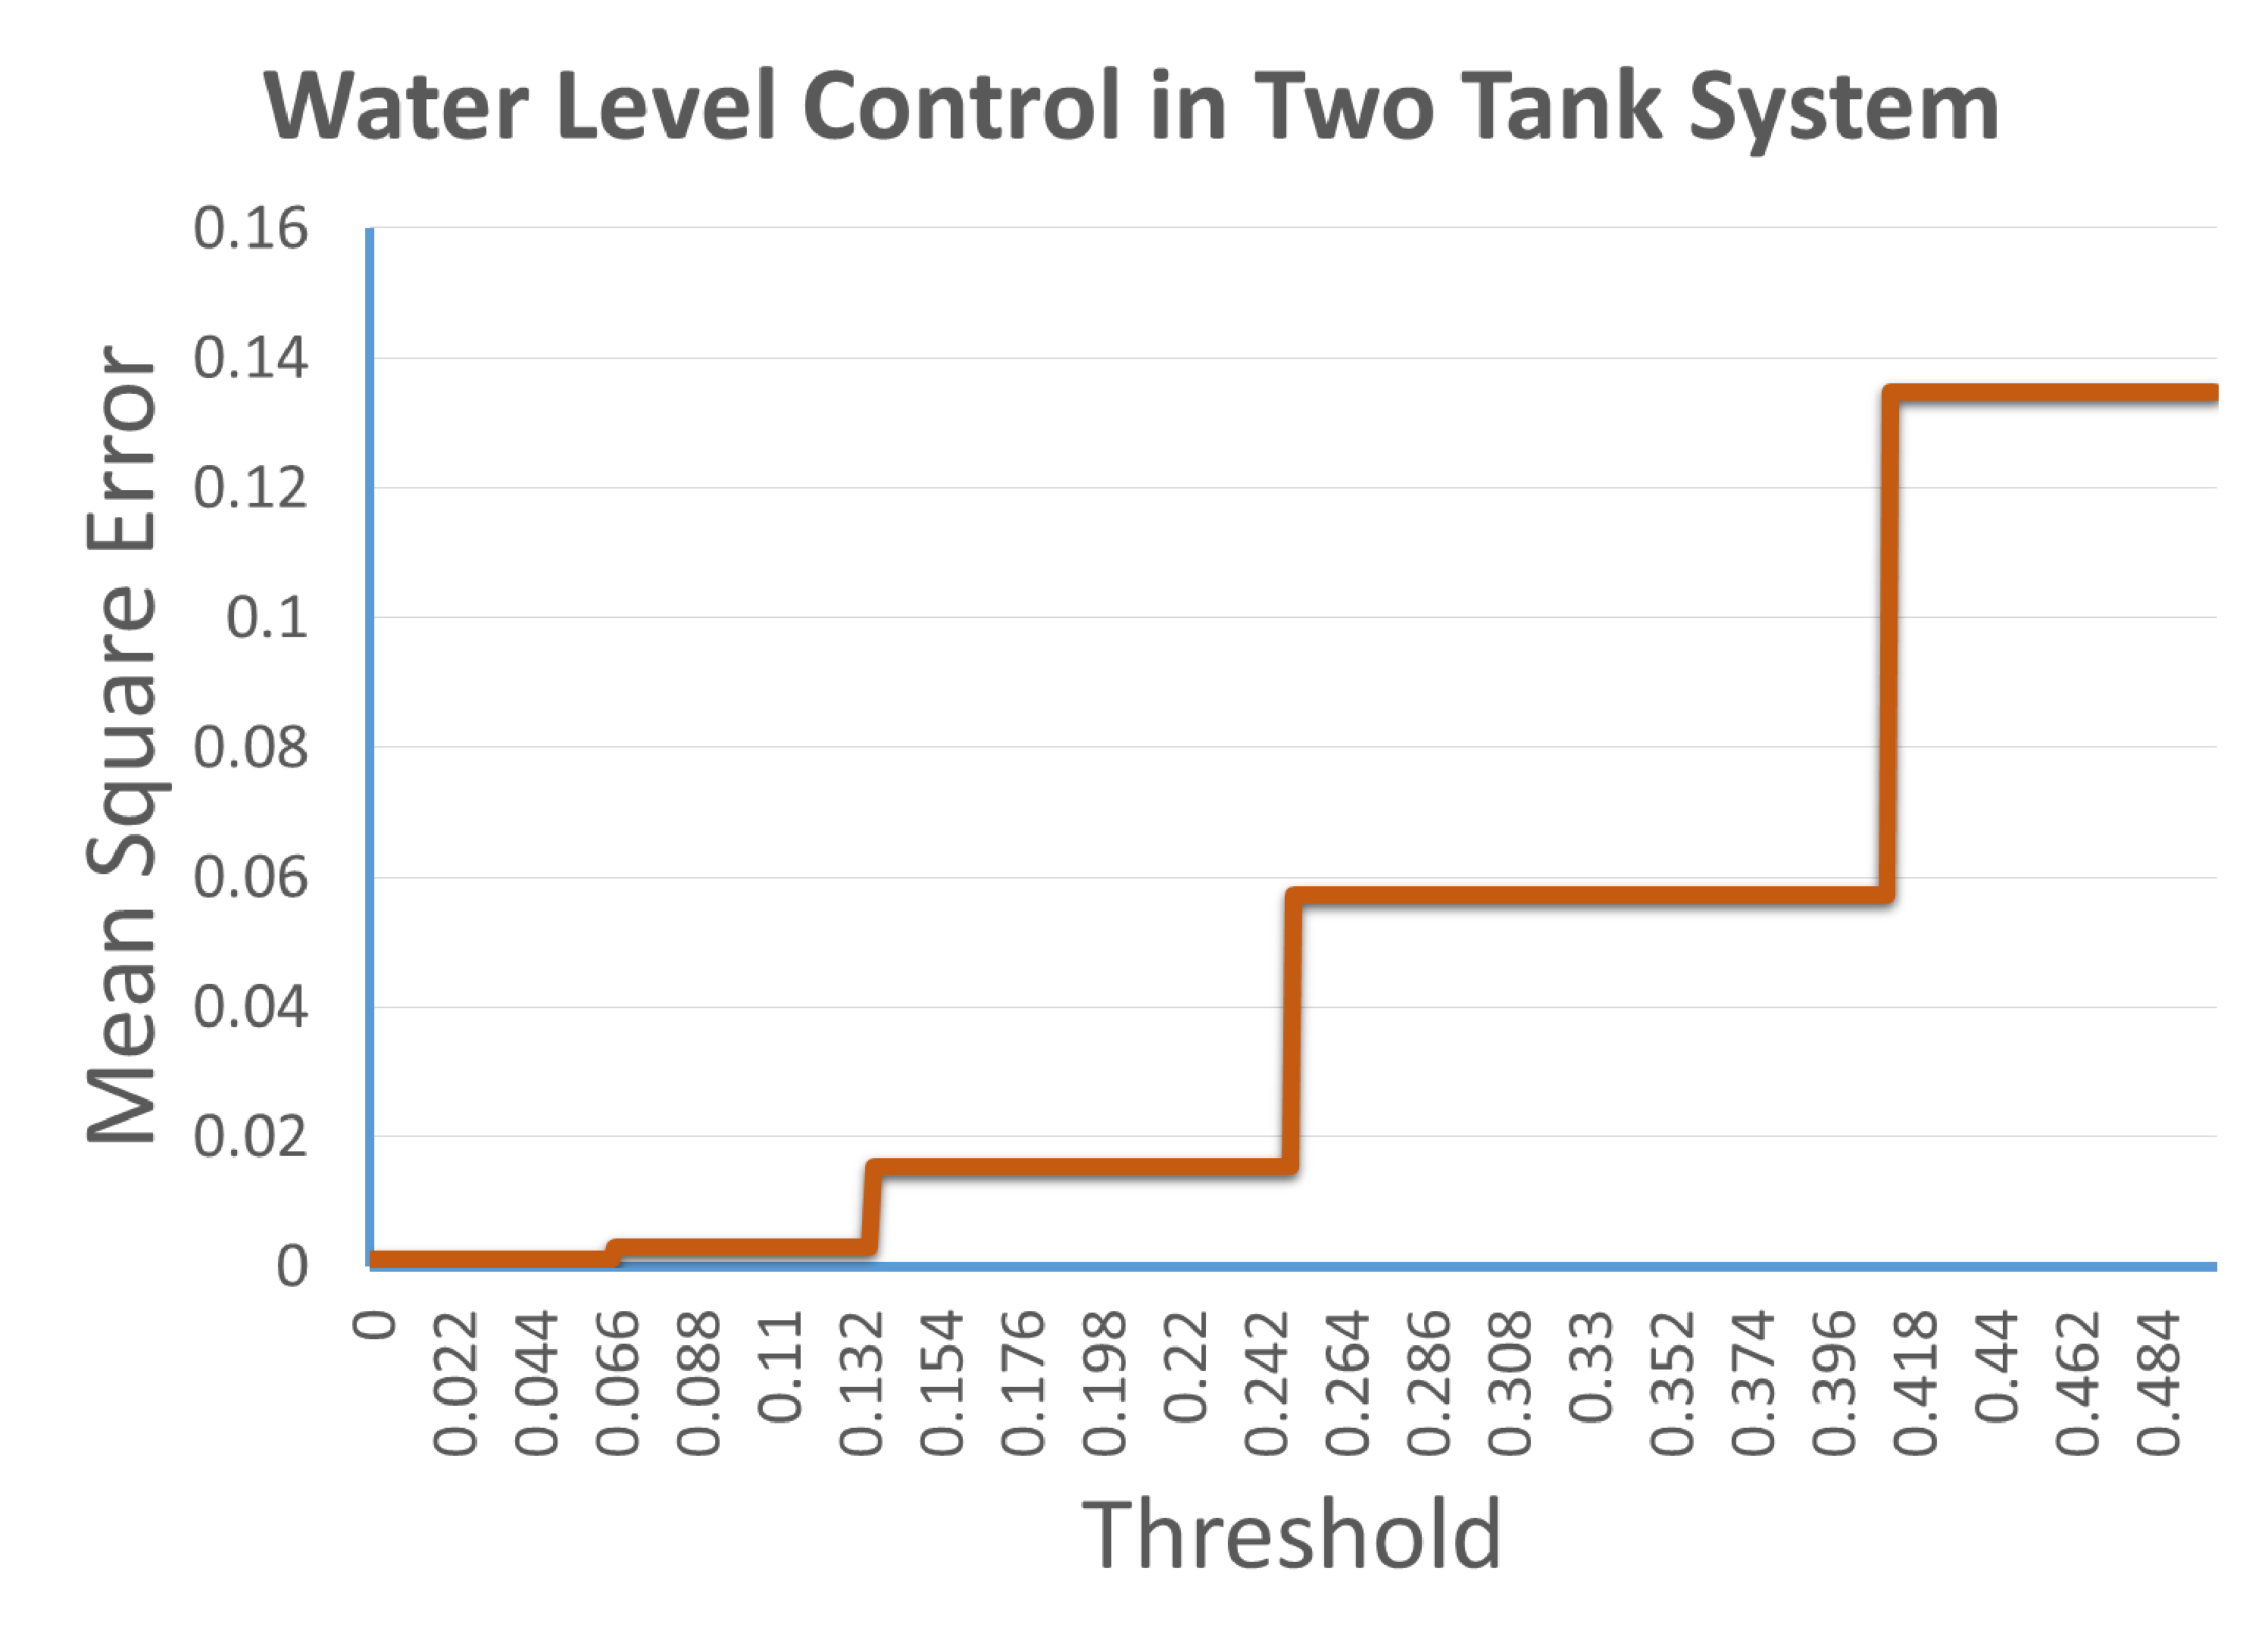
\includegraphics[width=0.55\linewidth]{Chapter2/chapter2/MSEvTH_Tank}} \\
	\subfloat[Truck Backer Control System]{\label{fig:MSEvTH_Truck}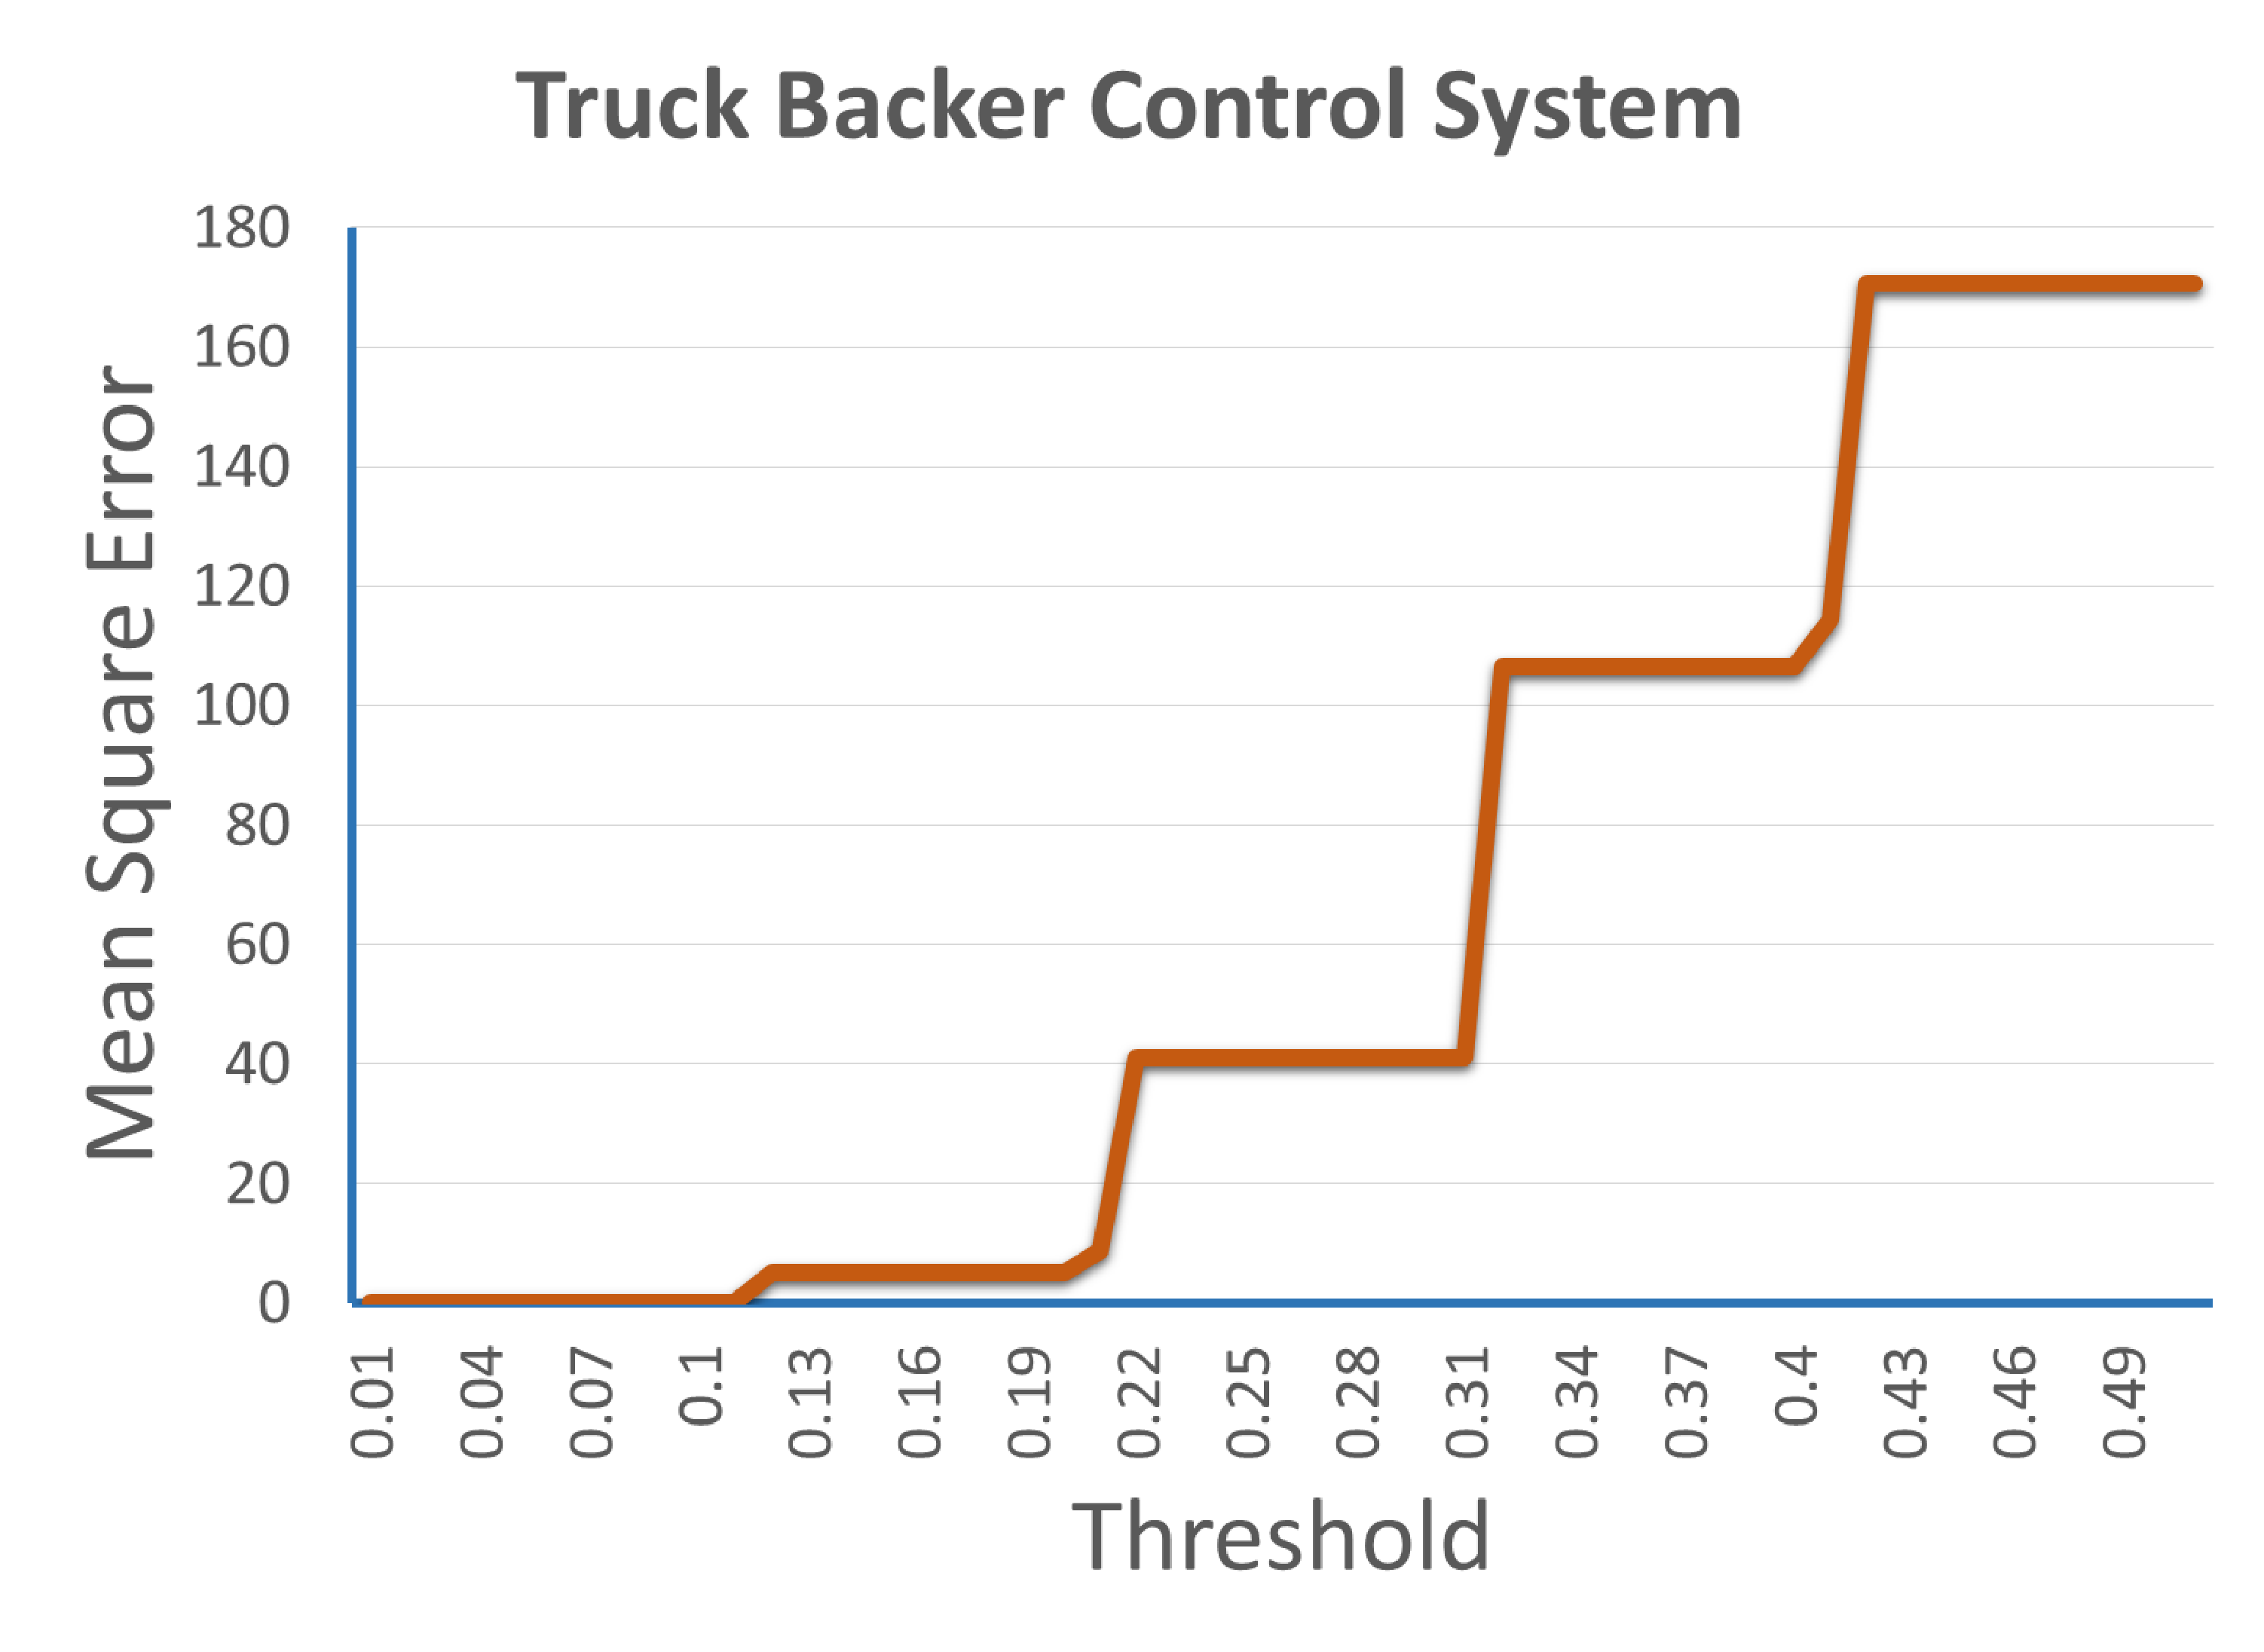
\includegraphics[width=0.55\linewidth]{Chapter2/chapter2/MSEvTH_Truck}}
	\caption{Dependency of MSE on threshold introduced in MT-FRHC Rule reduction technique for FIS structure file employed in FLC to control various systems. These systems considered are two input one output systems, no. of operations per inference is 16. }
	\label{fig:MSEvTH}
\end{figure}
In this section, the proposed MT-FRHC based G\hyp{}FLCS analyzed.  It is important to analyze the designed methodology on existing FLCS designs. Matlab Fuzzy Logic Toolbox (FLT) have been widely used to develop many fuzzy control applications. Every Matlab FLT uses a fuzzy parameter file called as \textit{fis} file which stores the FCP. In this analysis, the performance of the proposed MT-FRHC based G-FLCS is compared to Matlab FLT.

To analyze the performance of the proposed system, it was implemented on a test problem. Shiva Malla \cite{malla2012} used Matlab FLT to design a Fuzzy PI approximate controller for speed control of an Armature Controlled Direct Current (ACDC) motor. A web link to a FIS structure file used by Shiva Malla \cite{malla2012} for Fuzzy PI approximation to control ACDC motor is provided in Appendix-A. The Fuzzy PI Controller is a two-input one-output system with error and change in error ($\delta Error$) as the input and control signal as the output. The range of both the input space varies from $-1 $ to $ 1 $. he output ranges from $ -30 $ to $ 30 $. All possible combinations inputs with a step of 0.001 are sequentially introduced into the MT-FRHC based G-FLCS, and the correspond results are noted for threshold $ \tau = 0.2 $. A surface plot is generated from these observed results as shown in Figure \ref{fig:SPlot_MT-FRHC}. The x-axis represents the error ranging from 0 to 1 with a step size of 0.001, while the y-axis shows the change in error($\delta Error$) also ranging from 0 to 1 with a step size of 0.001. The output of the G-FLCS is plotted in the z-axis. Similarly, a surface plot is generated using Matlab FLT using the same FCP. This is presented in Figure \ref{fig:SPlot_MFT}. The individual error between these two system output is calculated and plotted in Figure \ref{fig:SPlot_Error}. The x and the y- axes, which represents the inputs remains same as in the other plots. However, the z-axis represents the absolute error between the system output generated from the proposed MT-FRHC based G-FLCS system and Matlab FLT. Considering Matlab MLT as the true value, it can be observed  MT-FRHC based G-FLCS produces a peak error of $ \pm 2 $ over an output range of $ \pm 30 $. At this moment, the proposed system produces a maximum of 6.67\% error.

The generality of a G\hyp{}FLCS can only be established once it is implemented on different FLCS designs. The proposed MT-FRHC based G-FLCS controller is tested similarly with two other benchmark control problems, namely, a water level control of a two tank system \cite{twotank2012} and a truck backer control system\cite{Passino2010}. Figure \ref{fig:SPlot_MT-FRHC_tank} shows the surface plot for output (on z-axis) of the MT-FRHC based G-FLCS system with respect to the water level (in x-axis) and input flow rate (y-axis). Figure \ref{fig:SPlot_MFT_tank} represents the surface plot for output (on z-axis) of the Matlab FLT system with respect to the water level (in x-axis) and input flow rate (y-axis). The surface plot of the error between these two systems is presented in Figure \ref{fig:SPlot_Error_tank}. It can be seen that for this particular example, MT-FRHC based G-FLCS produces a peak error of $ \pm 3\times10^{-15} $ over an output range of $ \pm 1 $. Now, the proposed system produces a negligibly small error that is very close to 0.

In Figure \ref{fig:SPlot_MT-FRHC_truck}, the surface plot for fuzzy output (on the z-axis) of the MT-FRHC based G-FLCS system is plotted for a truck backer system. Figure \ref{fig:SPlot_MFT_truck} represents the surface plot for fuzzy output (on the z-axis) of the Matlab FLT system for the same system. The surface plot of the error between these two systems is presented in Figure \ref{fig:SPlot_Error_truck}. It can be seen in error surface plot that, MT-FRHC based G-FLCS produces a peak error of $ \pm 5 $ over an output range of $ \pm 40 $. At this moment, the proposed system produces an error of 1.25\%.

Following the previous analysis, the same benchmark control problems were employed to draw dependency between the threshold $ \tau $ and mean square error.
It is analytically evident that MSE is proportional to the threshold $ \tau $. However, the computational complexity of G-FLCS is inversely proportional to $ \tau $. In an ideal scenario, a G-FLCS encounters following optimization problem.
\begin{itemize}
	\item Lower value of $ \tau $ to reduce MSE.
	\item Higher value of $ \tau $ to reduce computational complexity.
\end{itemize}
For MT-FRHC based G-FLCS, MSE is calculated with respect to Matlab FLT against different threshold values. In Figure \ref{fig:MSEvTH}, the trend of MSE with increase in $\tau$ is presented for Fuzzy PI Control of ACDC motor \cite{malla2012}, a water level control of a two tank system \cite{twotank2012} and a truck backer control system\cite{Passino2010}. It can be observed that MSE of a system is variedly dependent on different FIS structure file at the constant threshold. Thereby, it can be safely inferred that $\tau$ has to be dynamically assigned to a G-FLCS depending on the system it is employed, and this factor cannot be generalized. As a result of this, selection of $\tau$ should be based on
\begin{itemize}
	\item accuracy demand from the system
	\item throughput time of the system
\end{itemize}

\section{Proposed MT-FRHC based G-FLCS Implementation and its Validation}
At this juncture, it is necessary to implement the proposed algorithm on a programmable device and validate the results. To achieve this, the proposed system is implemented on a TI TMS320C6748 DSP processor operating on 300 MHz with $ \tau = 0.2 $. For comparative analysis of the MT-FRHC based G-FLCS technique, the Overlapping Membership Function (OMF) based G-FLCS is also implemented on the same platform. A 4-input/1-output, 9 rule, COA defuzzification FLC was used for testing. A download link to this FCP is provided in Appendix-A. The timing analysis of this experiment conducted is presented at Table \ref{tab:ch2timing}. Timing analysis of this experiment was executed using Code Composer Studio Timing Profiler. This tool presented the machine cycles consumed during execution of the method. 

\begin{table}[h]
	\centering
	\caption{Hardware Implementation: Timing Analysis}
	\label{tab:ch2timing}
	\begin{tabular}{cccc}
		\hline \noalign{\vskip 1mm} 
		Sl. & Cycles & Time (ms) & FLIPS \\ \hline \noalign{\vskip 1mm} 
		1. & 43370 & 0.1445 & 6920.42 \\
		2. & 38546 & 0.1285 & 7782.10 \\
		3. & 38451 & 0.1282 & 7800.31 \\
		4. & 38182 & 0.1273 & 7853.6 \\
		5. & 37567 & 0.1282 & 7800.31 \\
		6. & 30944 & 0.1032 & 9689.5 \\
		7. & 38995 & 0.13 & 7692.3 \\
		8. & 38513 & 0.1286 & 7788.2 \\
		9. & 38595 & 0.1287 & 7770.00 \\
		10. & 38578 & 0.1286 & 7776.05 \\ \hline
	\end{tabular}
\end{table}

From the Table \ref{tab:ch2avgtiming} it can be observed that the execution time for MT-FRHC is 0.0259 ms per inferences compared to Overlapping Membership Function (OMF) with 0.0346 ms per inference. This implies that the number of fuzzy logic inferences per second (FLIPS) completed by the proposed technique is quite higher. It has been found that the MT-FRHC based G-FLCS achieved 27 \% higher performance in terms of speed compared to the OMF based G-FLCS. Table \ref{tab:ch2avgtiming} presents the timing analysis of the individual modules in the G-FLCS. It can be seen that fuzzifier consumes significant machine cycles in comparison to other modules. This is mostly because the code has been written in a sequential manner, and there is a single thread of fuzzifier that fuzzifies crisp data from all four input channels to fuzzy data sequentially. The cycle time for fuzzifier can be significantly improved by invoking multiple threads using TI Sys/Bios\footnote{TI Sys/Bios is a real-time operating system primarily developed for TI manufactured DSPs, ARM and other programmable devices.} . 

\begin{table}[h]
	\centering
	\caption{Hardware Implementation: Average Time Response}
	\label{tab:ch2avgtiming}
	\resizebox{0.9\linewidth}{!}{%
		\begin{tabular}{ccccccc}
			\hline \noalign{\vskip 1mm} 
			~ & Fuzzifier & Inference & Defuzzifier & Total & Time & FLIPS \\ \hline \noalign{\vskip 1mm} 
			~ & \multicolumn{4}{c|}{(Cycles)} & \multicolumn{1}{c|}{(ms)} & (Kilo) \\ \noalign{\vskip 1mm} \hline \noalign{\vskip 1mm} 
			MT-FRHC & 29393 & 1823 & 6332 & 38548 & 0.1285 & 7.8 \\ 
			OMF & 41843 & 2198 & 8565 & 52606 & 0.1754 & 5.7 \\ \hline \noalign{\vskip 1mm} 
		\end{tabular}
	}
\end{table}


\section{Summary}
In this chapter, a theoretical analysis of M-FRHC and MT-FRHC has been elaborated which was aimed at countering the significant limitations of predominant FRHC technique. Simulation results indicate that the proposed scheme can be implemented on hardware G\hyp{}FLCS and replace the prevailing FRHC as rule reduction technique. This algorithm has managed to improve controller accuracy with a significant decrease in the computational complexity. This analysis portrays promising results in favour of MT-FRHC in both fronts and its utility in G-FLC design is dominantly inferred. This method also provides a platform where users can vary the number of overlaps and threshold value for fuzzifier of a G-FLCS in real-time. It has also been shown that with varying number of overlapping membership functions, the number of operations in the inference engine can be controlled. The introduction of threshold in fuzzifier will eradicate insignificant computations in the system. These programmable features in MT-FRHC provide added control on the performance of the controller itself and a user can steer the MT-FRHC based G-FLCS to the performance with better efficiency.